% !TeX document-id = {8f46a525-8bce-4928-9b8c-e09cd7063361}
% !TeX spellcheck = en-US
% !TeX encoding = utf8
% !TeX program = pdflatex
% !BIB program = biber
% -*- coding:utf-8 mod:LaTeX -*-


% vv  scroll down to line 200 for content  vv


\let\ifdeutsch\iffalse
\let\ifenglisch\iftrue
% EN: This file is loaded before the \documentclass command in the main document

% EN: The following package allows \\ at the title page
%     For more information see https://github.com/latextemplates/scientific-thesis-cover/issues/4
\RequirePackage{kvoptions-patch}

\ifenglisch
  \PassOptionsToClass{numbers=noenddot}{scrbook}
\else
  %()Aus scrguide.pdf - der Dokumentation von KOMA-Script)
  %Nach DUDEN steht in Gliederungen, in denen ausschließlich arabische Ziffern für die Nummerierung
  %verwendet werden, am Ende der Gliederungsnummern kein abschließender Punkt
  %(siehe [DUD96, R3]). Wird hingegen innerhalb der Gliederung auch mit römischen Zahlen
  %oder Groß- oder Kleinbuchstaben gearbeitet, so steht am Ende aller Gliederungsnummern ein
  %abschließender Punkt (siehe [DUD96, R4])
  \PassOptionsToClass{numbers=autoendperiod}{scrbook}
\fi

% Warns about outdated packages and missing caption declarations
% See https://www.ctan.org/pkg/nag
\RequirePackage[l2tabu, orthodox]{nag}

%DE: Neue deutsche Trennmuster
%    Siehe http://www.ctan.org/pkg/dehyph-exptl und http://projekte.dante.de/Trennmuster/WebHome
%    Nur für pdflatex, nicht für lualatex
\RequirePackage{ifluatex}
\ifluatex
  % do not load anything
\else
  \ifdeutsch
    \RequirePackage[ngerman=ngerman-x-latest]{hyphsubst}
  \fi
\fi

\documentclass[
  % fontsize=11pt is the standard
  a4paper,  % Standard format - only KOMAScript uses paper=a4 - https://tex.stackexchange.com/a/61044/9075
  twoside,  % we are optimizing for both screen and two-side printing. So the page numbers will jump, but the content is configured to stay in the middle (by using the geometry package)
  bibliography=totoc,
  %               idxtotoc,   %Index ins Inhaltsverzeichnis
  %               liststotoc, %List of X ins Inhaltsverzeichnis, mit liststotocnumbered werden die Abbildungsverzeichnisse nummeriert
  headsepline,
  cleardoublepage=empty,
  parskip=half,
  %               draft    % um zu sehen, wo noch nachgebessert werden muss - wichtig, da Bindungskorrektur mit drin
  draft=false,
  open=any
]{scrbook}
% !TeX encoding = utf8
% -*- coding:utf-8 mod:LaTeX -*-

% EN: This file includes basic packages and sets options. The order of package
%     loading is important

% DE: In dieser Datei werden zuerst die benoetigten Pakete eingebunden und
%     danach diverse Optionen gesetzt. Achtung Reihenfolge ist entscheidend!


% EN: Styleguide:
% - English comments are prefixed with "EN", German comments are prefixed with "DE"
% - Prefixed headings define the language for the subsequent paragraphs
% - It is tried to organize packages in blocks. Bocks are separated by two empty lines.

% DE: Styleguide:
%
% Ein sehr kleiner Styleguide. Packages werden in Blöcken organisiert.
% Zwischen zwei Blöcken sind 2 Leerzeilen!


% EN: Enable copy and paste of text from the PDF
%     Only required for pdflatex. It "just works" in the case of lualatex.
%     mmap enables mathematical symbols, but does not work with the newtx font set
%     See: https://tex.stackexchange.com/a/64457/9075
%     Other solutions outlined at http://goemonx.blogspot.de/2012/01/pdflatex-ligaturen-und-copynpaste.html and http://tex.stackexchange.com/questions/4397/make-ligatures-in-linux-libertine-copyable-and-searchable
%     Trouble shooting outlined at https://tex.stackexchange.com/a/100618/9075

\ifluatex
\else
  \usepackage{cmap}
\fi


% EN: File encoding
% DE: Codierung
%     Wir sind im 21 Jahrhundert, utf-8 löst so viele Probleme.
%
% Mit UTF-8 funktionieren folgende Pakete nicht mehr. Bitte beachten!
%   * fancyvrb mit §
%   * easylist -> http://www.ctan.org/tex-archive/macros/latex/contrib/easylist/
\ifluatex
  % EN: See https://tex.stackexchange.com/a/158517/9075
  %     Not required, because of usage of fontspec package
  %\usepackage[utf8]{luainputenc}
\else
  \usepackage[utf8]{inputenc}
\fi


% DE: Parallelbetrieb tex4ht und pdflatex

\makeatletter
\@ifpackageloaded{tex4ht}{
  \def\iftex4ht{\iftrue}
}{
  \def\iftex4ht{\iffalse}
}
\makeatother


% EN: Mathematics
% DE: Mathematik
%
% DE: Viele Mathematik-Sachen. Siehe https://texdoc.net/pkg/amsmath
%
% EN: Options must be passed this way, otherwise it does not work with glossaries
% DE: fleqn (=Gleichungen linksbündig platzieren) funktioniert nicht direkt. Es muss noch ein Patch gemacht werden:
\PassOptionsToPackage{fleqn,leqno}{amsmath}
%
% DE: amsmath Muss nicht mehr geladen werden, da es von newtxmath automatisch geladen wird
% \usepackage{amsmath}


%% EN: Fonts
%% DE: Schriften
%%
%% !!! If you change the font, be sure that words such as "workflow" can
%% !!! still be copied from the PDF. If this is not the case, you have
%% !!! to use glyphtounicode. See comment at cmap package


% EN: Times Roman for all text
\ifluatex
  % source: Second proposed fix from the following answer: https://tex.stackexchange.com/a/394137
  \usepackage[no-math]{fontspec}
  \setmainfont{TeXGyreTermes-Regular}[
       BoldFont       = TeXGyreTermes-Bold ,
       ItalicFont     = TeXGyreTermes-Italic ,
       BoldItalicFont = TeXGyreTermes-BoldItalic,
       NFSSFamily     = ntxtlf]
  \setsansfont{TeX Gyre Heros Regular}[
       Scale=.9,
       BoldFont       = TeX Gyre Heros Bold,
       ItalicFont     = TeX Gyre Heros Italic,
       BoldItalicFont = TeX Gyre Heros BoldItalic]
  \setmonofont[StylisticSet={1,3},Scale=.9]{inconsolata}
  \RequirePackage{newtxmath}
\else
  \RequirePackage{newtxtext}
  \RequirePackage{newtxmath}
  % EN: looks good with times, but no equivalent for lualatex found,
  %     therefore replaced with inconsolata
  %\RequirePackage[zerostyle=b,scaled=.9]{newtxtt}
  \RequirePackage[varl,scaled=.9]{inconsolata}
\fi

% EN: Fallback font - if the subsequent font packages do not define a font (e.g., monospaced)
%     This is the modern package for "Computer Modern".
%     In case this gets activated, one has to switch from cmap package to glyphtounicode (in the case of pdflatex)
% DE: Fallback-Schriftart
%\usepackage[%
%    rm={oldstyle=false,proportional=true},%
%    sf={oldstyle=false,proportional=true},%
%    tt={oldstyle=false,proportional=true,variable=true},%
%    qt=false%
%]{cfr-lm}

% EN: Headings are typset in Helvetica (which is similar to Arial)
% DE: Schriftart fuer die Ueberschriften - ueberschreibt lmodern
%\usepackage[scaled=.95]{helvet}

% DE: Für Schreibschrift würde tun, muss aber nicht
%\usepackage{mathrsfs} %  \mathscr{ABC}

% EN: Font for the main text
% DE: Schriftart fuer den Fliesstext - ueberschreibt lmodern
%     Linux Libertine, siehe http://www.linuxlibertine.org/
%     Packageparamter [osf] = Minuskel-Ziffern
%     rm = libertine im Brottext, Linux Biolinum NICHT als serifenlose Schrift, sondern helvet (von oben) beibehalten
%\usepackage[rm]{libertine}

% EN: Alternative Font: Palantino. It is recommeded by Prof. Ludewig for German texts
% DE: Alternative Schriftart: Palantino, Packageparamter [osf] = Minuskel-Ziffern
%     Bitte nur in deutschen Texten
%\usepackage{mathpazo} %ftp://ftp.dante.de/tex-archive/fonts/mathpazo/ - Tipp aus DE-TEX-FAQ 8.2.1

% DE: Schriftart fuer Programmcode - ueberschreibt lmodern
%     Falls auskommentiert, wird die Standardschriftart lmodern genommen
%     Fuer schreibmaschinenartige Schluesselwoerter in den Listings - geht bei alten Installationen nicht, da einige Fontshapes (<>=) fehlen
%\usepackage[scaled=.92]{luximono}
%\usepackage{courier}
% DE: BeraMono als Typewriter-Schrift, Tipp von http://tex.stackexchange.com/a/71346/9075
%\usepackage[scaled=0.83]{beramono}

% EN: backticks (`) are rendered as such in verbatim environments.
%     See following links for details:
%     - https://tex.stackexchange.com/a/341057/9075
%     - https://tex.stackexchange.com/a/47451/9075
%     - https://tex.stackexchange.com/a/166791/9075
\usepackage{upquote}

% DE: Symbole
%
%\usepackage[geometry]{ifsym} % \BigSquare
%\usepackage{mathabx}
%\usepackage{stmaryrd} %fuer \ovee, \owedge, \otimes
%\usepackage{marvosym} %fuer \Writinghand %patched to not redefine \Rightarrow
%\usepackage{mathrsfs} %mittels \mathscr{} schoenen geschwungenen Buchstaben erzeugen
%\usepackage{calrsfs} %\mathcal{} ein bisserl dickeren buchstaben erzeugen - sieht net so gut aus.
%durch mathpazo ist das schon definiert

%
%\usepackage{amssymb}

% EN: For \texttrademark{}
\usepackage{textcomp}

% EN: name-clashes von marvosym und mathabx vermeiden:
\def\delsym#1{%
  %  \expandafter\let\expandafter\origsym\expandafter=\csname#1\endcsname
  %  \expandafter\let\csname orig#1\endcsname=\origsym
  \expandafter\let\csname#1\endcsname=\relax
}

%\usepackage{pifont}
%\usepackage{bbding}
%\delsym{Asterisk}
%\delsym{Sun}\delsym{Mercury}\delsym{Venus}\delsym{Earth}\delsym{Mars}
%\delsym{Jupiter}\delsym{Saturn}\delsym{Uranus}\delsym{Neptune}
%\delsym{Pluto}\delsym{Aries}\delsym{Taurus}\delsym{Gemini}
%\delsym{Rightarrow}
%\usepackage{mathabx} - Ueberschreibt leider zu viel - und die \le-Zeichen usw. sehen nicht gut aus!


% EN: Modern font encoding
%     Has to be loaded AFTER any font packages. See https://tex.stackexchange.com/a/2869/9075.
\ifluatex
\else
  \usepackage[T1]{fontenc}
\fi
%


% EN: Character protrusion and font expansion. See http://www.ctan.org/tex-archive/macros/latex/contrib/microtype/
% DE: Optischer Randausgleich und Grauwertkorrektur

\usepackage[
  babel=true, % EN: Enable language-specific kerning. Take language-settings from the languge of the current document (see Section 6 of microtype.pdf)
  expansion=alltext,
  protrusion=alltext-nott, % EN: Ensure that at listings, there is no change at the margin of the listing
  final % EN: Always enable microtype, even if in draft mode. This helps finding bad boxes quickly.
        %     In the standard configuration, this template is always in the final mode, so this option only makes a difference if "pros" use the draft mode
]{microtype}


% EN: \texttt{test -- test} keeps the "--" as "--" (and does not convert it to an en dash)
\DisableLigatures{encoding = T1, family = tt* }

% DE: fuer microtype
% DE: tracking=true muss als Parameter des microtype-packages mitgegeben werden
% DE: Deaktiviert, da dies bei Algorithmen seltsam aussieht

%\DeclareMicrotypeSet*[tracking]{my}{ font = */*/*/sc/* }%
%\SetTracking{ encoding = *, shape = sc }{ 45 }
% DE: Hier wird festgelegt,
%     dass alle Passagen in Kapitälchen automatisch leicht
%     gesperrt werden.
%     Quelle: http://homepage.ruhr-uni-bochum.de/Georg.Verweyen/pakete.html
%    Deaktiviert, da sonst "BPEL", "BPMN" usw. wirklich komisch aussehen.
%     Macht wohl nur bei geisteswissenschaftlichen Arbeiten Sinn.


% EN: amsmath teaks


% EN: Fixes bugs in AMS math
%     Corrently conflicts with unicode-math
% \usepackage{mathtools}

%\numberwithin{equation}{section}
%\renewcommand{\theequation}{\thesection.\Roman{equation}}

% EN: work-around ams-math problem with align and 9 -> 10. Does not work with glossaries, No visual changes.
%\addtolength\mathindent{1em}


% EN: For theorems, replacement for amsthm
\usepackage[amsmath,hyperref]{ntheorem}
\theorempreskipamount 2ex plus1ex minus0.5ex
\theorempostskipamount 2ex plus1ex minus0.5ex
\theoremstyle{break}
\newtheorem{definition}{Definition}[section]


% CTAN: https://ctan.org/pkg/lccaps
% Doc: http://texdoc.net/pkg/lccaps
%
% Required for DE/EN \initialism
\usepackage{lccaps}


% EN: Defintion of colors. Argument "hyperref" is not used as we do not want to change border colors of links: Links are not colored anymore.
% DE: Farbdefinitionen
\usepackage[dvipsnames]{xcolor}


% EN: Required for custom acronyms/glossaries style.
%     Left aligned Columns in tables with fixed width.
%     See http://tex.stackexchange.com/questions/91566/syntax-similar-to-centering-for-right-and-left
\usepackage{ragged2e}


% DE: Wichtig, ansonsten erscheint "No room for a new \write"
\usepackage{scrwfile}


% EN: Support for language-specific hyphenation
% DE: Neue deutsche Rechtschreibung und Literatur statt "Literature"
%     Die folgende Einstellung ist der Nachfolger von ngerman.sty
\ifdeutsch
  % DE: letzte Sprache ist default, Einbindung von "american" ermöglicht \begin{otherlanguage}{amercian}...\end{otherlanguage} oder \foreignlanguage{american}{Text in American}
  %     Siehe auch http://tex.stackexchange.com/a/50638/9075
  \usepackage[american,main=ngerman]{babel}
  % Ein "abstract" ist eine "Kurzfassung", keine "Zusammenfassung"
  \addto\captionsngerman{%
    \renewcommand\abstractname{Kurzfassung}%
  }
  \ifluatex
    % EN: conditionally disable ligatures. See https://github.com/latextemplates/scientific-thesis-template/issues/54
    %     for a discussion
    \usepackage[ngerman]{selnolig}
  \fi
\else
  % EN: Set English as language and allow to write hyphenated"=words
  %     `american`, `english` and `USenglish` are synonyms for babel package (according to https://tex.stackexchange.com/questions/12775/babel-english-american-usenglish).
  %      "english" has to go last to set it as default language
  \usepackage[ngerman,main=english]{babel}
  % EN: Hint by http://tex.stackexchange.com/a/321066/9075 -> enable "= as dashes
  \addto\extrasenglish{\languageshorthands{ngerman}\useshorthands{"}}
  \ifluatex
    % EN: conditionally disable ligatures. See https://github.com/latextemplates/scientific-thesis-template/issues/54
    %     for a discussion
    \usepackage[english]{selnolig}
  \fi
\fi
%


% EN: For easy quotations: \enquote{text}
%     This package is very smart when nesting is applied, otherwise textcmds (see below) provides a shorter command
%     Note that this package results in a warning when it is loaded before minted (actually fvextra).
% DE: Anführungszeichen
%     Zitate in \enquote{...} setzen, dann werden automatisch die richtigen Anführungszeichen verwendet.
%     Dieses package erzeugt eine Warnung, wenn es vor minted (genauer fvextra) geladen wird.
\usepackage{csquotes}


% EN: For even easier quotations: \qq{text}.
%     Is not smart in the case of nesting, but good enough for the most cases
\usepackage{textcmds}
\ifdeutsch
  % EN: German quotes are different. So do not use the English quotes, but the ones provided by the csquotes package.
  \renewcommand{\qq}[1]{\enquote{#1}}
\fi


% EN: extended enumarations
% DE: erweitertes Enumerate
\usepackage{paralist}


% DE: Gestaltung der Kopf- und Fußteilen

\usepackage[automark]{scrlayer-scrpage}

\automark[section]{chapter}
\setkomafont{pageheadfoot}{\normalfont\sffamily}
\setkomafont{pagenumber}{\normalfont\sffamily}

% DE: funktioniert nicht: Alle Linien sind hier weg
%\setheadsepline[.4pt]{.4pt}


% DE: Intelligentes Leerzeichen um hinter Abkürzungen die richtigen Abstände zu erhalten, auch leere.
%     Siehe commands.tex \gq{}
\usepackage{xspace}
% DE: Macht \xspace und \enquote kompatibel
\makeatletter
\xspaceaddexceptions{\grqq \grq \csq@qclose@i \} }
\makeatother


\newcommand{\eg}{e.\,g.,\ }
\newcommand{\ie}{i.\,e.,\ }


% EN: introduce \powerset - hint by http://matheplanet.com/matheplanet/nuke/html/viewtopic.php?topic=136492&post_id=997377
\DeclareFontFamily{U}{MnSymbolC}{}
\DeclareSymbolFont{MnSyC}{U}{MnSymbolC}{m}{n}
\DeclareFontShape{U}{MnSymbolC}{m}{n}{
  <-6>    MnSymbolC5
  <6-7>   MnSymbolC6
  <7-8>   MnSymbolC7
  <8-9>   MnSymbolC8
  <9-10>  MnSymbolC9
  <10-12> MnSymbolC10
  <12->   MnSymbolC12%
}{}
\DeclareMathSymbol{\powerset}{\mathord}{MnSyC}{180}


% EN: Package for the appendix
% DE: Anhang
\usepackage{appendix}
%[toc,page,title,header]
%


% EN: Graphics
% DE: Grafikeinbindungen
%
% EN: The parameter "pdftex" is not required
\usepackage{graphicx}
\graphicspath{{\getgraphicspath}}
\newcommand{\getgraphicspath}{graphics/}


% EN: Enables inclusion of SVG graphics - 1:1 approach
%    This is NOT the approach of https://ctan.org/pkg/svg-inkscape,
%     which allows text in SVG to be typeset using LaTeX
%     We just include the SVG as is.
\usepackage{epstopdf}
\epstopdfDeclareGraphicsRule{.svg}{pdf}{.pdf}{%
  inkscape -z -D --file=#1 --export-pdf=\OutputFile
}


% EN: Enables inclusion of SVG graphics - text-rendered-with-LaTeX-approach
%     This is the approach of https://ctan.org/pkg/svg-inkscape,
\newcommand{\executeiffilenewer}[3]{%
  \IfFileExists{#2}
  {
    %\message{file #2 exists}
    \ifnum\pdfstrcmp{\pdffilemoddate{#1}}%
      {\pdffilemoddate{#2}}>0%
      {\immediate\write18{#3}}
    \else
      {%\message{file up to date #2}
      }
    \fi%
  }{
    %\message{file #2 doesn't exist}
    %\message{argument: #3}
    %\immediate\write18{echo "test" > xoutput.txt}
    \immediate\write18{#3}
  }
}
\newcommand{\includesvg}[1]{%
  \executeiffilenewer{#1.svg}{#1.pdf}%
  {
    inkscape -z -D --file=\getgraphicspath#1.svg %
    --export-pdf=\getgraphicspath#1.pdf --export-latex}%
  \input{\getgraphicspath#1.pdf_tex}%
}


% EN: Enable typesetting values with SI units.
\ifdeutsch
  \usepackage[mode=text,group-minimum-digits=4]{siunitx}
  \sisetup{locale=DE}
\else
  \usepackage[mode=text,group-minimum-digits=4,group-separator={,}]{siunitx}
  \sisetup{locale=US}
\fi


% EN: Extensions for tables
% DE: Tabellenerweiterungen
\usepackage{array} %increases tex's buffer size and enables ``>'' in tablespecs
\usepackage{longtable}
\usepackage{dcolumn} %Aligning numbers by decimal points in table columns
\ifdeutsch
  \newcolumntype{d}[1]{D{.}{,}{#1}}
\else
  \newcolumntype{d}[1]{D{.}{.}{#1}}
\fi
\setlength{\extrarowheight}{1pt}


% DE: Eine Zelle, die sich über mehrere Zeilen erstreckt.
%     Siehe Beispieltabelle in Kapitel 2
\usepackage{multirow}


% DE: Fuer Tabellen mit Variablen Spaltenbreiten
%\usepackage{tabularx}
%\usepackage{tabulary}


% EN: Links behave as they should. Enables "\url{...}" for URL typesettings.
%     Allow URL breaks also at a hyphen, even though it might be confusing: Is the "-" part of the address or just a hyphen?
%     See https://tex.stackexchange.com/a/3034/9075.
% DE: Links verhalten sich so, wie sie sollen
%     Zeilenumbrüche bei URLs auch bei Bindestrichen erlauben, auch wenn es verwirrend sein könnte: Gehört der Bindestrich zur URL oder ist es ein Trennstrich?
%     Siehe https://tex.stackexchange.com/a/3034/9075.
\usepackage[hyphens]{url}
%
%  EN: When activated, use text font as url font, not the monospaced one.
%      For all options see https://tex.stackexchange.com/a/261435/9075.
% \urlstyle{same}
%
% EN: Hint by http://tex.stackexchange.com/a/10419/9075.
\makeatletter
\g@addto@macro{\UrlBreaks}{\UrlOrds}
\makeatother


% DE: Index über Begriffe, Abkürzungen
%\usepackage{makeidx} makeidx ist out -> http://xindy.sf.net verwenden


% DE: lustiger Hack fuer das Abkuerzungsverzeichnis
%     nach latex durchlauf folgendes ausfuehren
%     makeindex ausarbeitung.nlo -s nomencl.ist -o ausarbeitung.nls
%     danach nochmal latex
%\usepackage{nomencl}
%    \let\abk\nomenclature %Deutsche Ueberschrift setzen
%          \renewcommand{\nomname}{List of Abbreviations}
%        %Punkte zw. Abkuerzung und Erklaerung
%          \setlength{\nomlabelwidth}{.2\hsize}
%          \renewcommand{\nomlabel}[1]{#1 \dotfill}
%        %Zeilenabstaende verkleinern
%          \setlength{\nomitemsep}{-\parsep}
%    \makenomenclature


% EN: Logic for TeX - enables if-then-else in commands
% DE: Logik für TeX
%     FÜr if-then-else @ commands.tex
\usepackage{ifthen}


% EN: Code Listings
% DE: Listings
\usepackage{color}
\definecolor{pblue}{rgb}{0.13,0.13,1}
\definecolor{pgreen}{rgb}{0,0.5,0}
\definecolor{pred}{rgb}{0.9,0,0}
\definecolor{pgrey}{rgb}{0.46,0.45,0.48}
\usepackage{listings}
\lstset{language=Java,
	showspaces=false,
	showtabs=false,
	breaklines=true,
	showstringspaces=false,
	breakatwhitespace=true,
	commentstyle=\color{pgreen},
	keywordstyle=\color{pblue},
	stringstyle=\color{pred},
	basicstyle=\linespread{1.5}\ttfamily,
	tabsize=2,
	moredelim=[il][\textcolor{pgrey}]{$$},
	moredelim=[is][\textcolor{pgrey}]{\%\%}{\%\%}
}

\ifluatex
\else
  % EN: Enable UTF-8 support - see https://tex.stackexchange.com/q/419327/9075
  \usepackage{listingsutf8}
  \lstset{inputencoding=utf8/latin1}
\fi

\ifdeutsch
  \renewcommand{\lstlistlistingname}{Verzeichnis der Listings}
\fi


% EN: Alternative to listings could be fancyvrb. Can be used together.
% DE: Alternative zu Listings ist fancyvrb. Kann auch beides gleichzeitig benutzt werden.
\usepackage{fancyvrb}
%
% EN: Font size for the normal text
% DE: Groesse fuer den Fliesstext. Falls deaktiviert: \normalsize
%\fvset{fontsize=\small}
%
% DE: Somit kann im Text ganz einfach §verbatim§ text gesetzt werden.
%     Disabled, because UTF-8 does not work any more and lualatex causes issues
%\DefineShortVerb{\§}
%
% EN: Shrink font size of listings
\RecustomVerbatimEnvironment{Verbatim}{Verbatim}{fontsize=\footnotesize}
\RecustomVerbatimCommand{\VerbatimInput}{VerbatimInput}{fontsize=\footnotesize}
%
% EN: Hack for fancyvrb based on http://newsgroups.derkeiler.com/Archive/Comp/comp.text.tex/2008-12/msg00075.html
%     Change of the solution: \Vref somehow collidated with cleveref/varioref as the output of \Vref{} was "Abschnitt 4.3 auf Seite 85"; therefore changed to \myVref -- so completely removed
%     See https://tex.stackexchange.com/q/132420/9075 for more information.
\newcommand{\Vlabel}[1]{\label[line]{#1}\hypertarget{#1}{}}
\newcommand{\lref}[1]{\hyperlink{#1}{\FancyVerbLineautorefname~\ref*{#1}}}


% EN: Tunings of captions for floats, listings, ...
% DE: Bildunterschriften bei floats genauso formatieren wie bei Listings
%     Anpassung wird unten bei den newfloat-Deklarationen vorgenommen
%     https://www.ctan.org/pkg/caption2 is superseeded by this package.
\usepackage{caption}


% EN: Provides rotating figures, where the PDF page is also turned
% DE: Ermoeglicht es, Abbildungen um 90 Grad zu drehen
%     Alternatives Paket: rotating Allerdings wird hier nur das Bild gedreht, während bei lscape auch die PDF-Seite gedreht wird.
%     Das Paket lscape dreht die Seite auch nicht
\usepackage{pdflscape}


% EN: Required for proper environments of fancyvrb and lstlistings
%    There is also the newfloat pacakge (recommended by minted), but we currently have no expericene with that
% DE: Wird für fancyvrb und für lstlistings verwendet
\usepackage{float}
%
% EN: Alternative to float package
%\usepackage{floatrow}
% DE: zustäzlich für den Paramter [H] = Floats WIRKLICH da wo sie deklariert wurden paltzieren - ganz ohne Kompromisse
%     floatrow ist der Nachfolger von float
%     Allerdings macht floatrow in manchen Konstellationen Probleme. Deshalb ist das Paket deaktiviert.
%
% EN: See http://www.tex.ac.uk/cgi-bin/texfaq2html?label=floats
% DE: floats IMMER nach einer Referenzierung platzieren
%\usepackage{flafter}


% EN: Put footnotes below floats
%     Source: https://tex.stackexchange.com/a/32993/9075
\usepackage{stfloats}
\fnbelowfloat


% EN: For nested figures
% DE: Fuer Abbildungen innerhalb von Abbildungen
%     Ersetzt die Pakete subfigure und subfig - siehe https://tex.stackexchange.com/a/13778/9075
\usepackage[hypcap=true]{subcaption}


% EN: Extended support for footnotes
% DE: Fußnoten
%
%\usepackage{dblfnote}  %Zweispaltige Fußnoten
%
% Keine hochgestellten Ziffern in der Fußnote (KOMA-Script-spezifisch):
%\deffootnote[1.5em]{0pt}{1em}{\makebox[1.5em][l]{\bfseries\thefootnotemark}}
%
% Abstand zwischen Fußnoten vergrößern:
%\setlength{\footnotesep}{.85\baselineskip}
%
% EN: Following command disables the separting line of the footnote
% DE: Folgendes Kommando deaktiviert die Trennlinie zur Fußnote
%\renewcommand{\footnoterule}{}
%
\addtolength{\skip\footins}{\baselineskip} % Abstand Text <-> Fußnote
%
% Fußnoten immer ganz unten auf einer \raggedbottom-Seite
% fnpos kommt aus dem yafoot package
\usepackage{fnpos}
\makeFNbelow
\makeFNbottom


% EN: Variable page heights
% DE: Variable Seitenhöhen zulassen
\raggedbottom


% DE: Falls die Seitenzahl bei einer Referenz auf eine Abbildung nur dann angegeben werden soll,
%     falls sich die Abbildung nicht auf der selben Seite befindet...
\iftex4ht
  %tex4ht does not work well with vref, therefore we emulate vref behavior
  \newcommand{\vref}[1]{\ref{#1}}
\else
  \ifdeutsch
    \usepackage[ngerman]{varioref}
  \else
    \usepackage{varioref}
  \fi
\fi


% EN: More beautiful tables if one uses \toprule, \midrule, \bottomrule
% DE: Noch schoenere Tabellen als mit booktabs mit http://www.zvisionwelt.de/downloads.html
\usepackage{booktabs}
%
%\usepackage[section]{placeins}


% EN: Graphs and Automata
%
% TODO: Since version 3.0 (2013-10-01), it supports pdflatex via the auto-pst-pdf package
%       Requires -shell-escape
%\usepackage{gastex}


%\usepackage{multicol}

% DE: kollidiert mit diplomarbeit.sty
\usepackage{setspace} \doublespacing


% DE: biblatex statt bibtex
\usepackage[
  backend       = biber, %biber does not work with 64x versions alternative: bibtex8
  %minalphanames only works with biber backend
  sortcites     = true,
  bibstyle      = numeric,
  citestyle     = numeric,
  giveninits    = true,
  useprefix     = false, %"von, van, etc." will be printed, too. See below.
  minnames      = 1,
  minalphanames = 3,
  maxalphanames = 4,
  maxbibnames   = 99,
  maxcitenames  = 2,
  natbib        = true,
  eprint        = true,
  url           = true,
  doi           = true,
  isbn          = true,
  backref       = true]{biblatex}

% enable more breaks at URLs. See https://tex.stackexchange.com/a/134281.
\setcounter{biburllcpenalty}{7000}
\setcounter{biburlucpenalty}{8000}

\bibliography{bibliography}
%\addbibresource[datatype=bibtex]{bibliography.bib}

%Do not put "vd" in the label, but put it at "\citeauthor"
%Source: http://tex.stackexchange.com/a/30277/9075
\makeatletter
\AtBeginDocument{\toggletrue{blx@useprefix}}
\AtBeginBibliography{\togglefalse{blx@useprefix}}
\makeatother

%Thin spaces between initials
%http://tex.stackexchange.com/a/11083/9075
\renewrobustcmd*{\bibinitdelim}{\,}

%Keep first and last name together in the bibliography
%http://tex.stackexchange.com/a/196192/9075
\renewcommand*\bibnamedelimc{\addnbspace}
\renewcommand*\bibnamedelimd{\addnbspace}

%Replace last "and" by comma in bibliography
%See http://tex.stackexchange.com/a/41532/9075
\AtBeginBibliography{%
  \renewcommand*{\finalnamedelim}{\addcomma\space}%
}

\DefineBibliographyStrings{ngerman}{
  backrefpage  = {zitiert auf S\adddot},
  backrefpages = {zitiert auf S\adddot},
  andothers    = {et\ \addabbrvspace al\adddot},
  %Tipp von http://www.mrunix.de/forums/showthread.php?64665-biblatex-Kann-%DCberschrift-vom-Inhaltsverzeichnis-nicht-%E4ndern&p=293656&viewfull=1#post293656
  bibliography = {Literaturverzeichnis}
}

% EN: enable hyperlinked author names when using \citeauthor
%     source: http://tex.stackexchange.com/a/75916/9075
\DeclareCiteCommand{\citeauthor}
{\boolfalse{citetracker}%
  \boolfalse{pagetracker}%
  \usebibmacro{prenote}}
{\ifciteindex
  {\indexnames{labelname}}
  {}%
  \printtext[bibhyperref]{\printnames{labelname}}}
{\multicitedelim}
{\usebibmacro{postnote}}

% EN: natbib compatibility
%\newcommand{\citep}[1]{\cite{#1}}
%\newcommand{\citet}[1]{\citeauthor{#1} \cite{#1}}
% EN: Beginning of sentence - analogous to cleveref - important for names such as "zur Muehlen"
%\newcommand{\Citep}[1]{\cite{#1}}
%\newcommand{\Citet}[1]{\Citeauthor{#1} \cite{#1}}

% DE: Blindtext. Paket "blindtext" ist fortgeschritterner als "lipsum" und kann auch Mathematik im Text (http://texblog.org/2011/02/26/generating-dummy-textblindtext-with-latex-for-testing/)
%     kantlipsum (https://www.ctan.org/tex-archive/macros/latex/contrib/kantlipsum) ist auch ganz nett, aber eben auch keine Mathematik
%     Wird verwendet, um etwas Text zu erzeugen, um eine volle Seite wegen Layout zu sehen.
\usepackage[math]{blindtext}


% EN: Make LaTeX logos available by commands. E.g., \lualatex
%     Disabled, because currently causes \not= already defined
%\usepackage{dtk-logos}

% quick replacement:
\newcommand{\LuaLaTeX}{Lua\LaTeX\xspace}
\newcommand{\lualatex}{\LuaLaTeX}

% DE: Neue Pakete bitte VOR hyperref einbinden. Insbesondere bei Verwendung des
%     Pakets "index" wichtig, da sonst die Referenzierung nicht funktioniert.
%     Für die Indizierung selbst ist unter http://xindy.sourceforge.net
%     ein gutes Tool zu erhalten.
%     Hier also neue packages einbinden.
% EN: Add new packages at this place.


% EN: Provides hyperlinks
%     Option "unicode" fixes umlauts in the PDF bookmarks - see https://tex.stackexchange.com/a/338770/9075
%
% DE: Erlaubt Hyperlinks im Dokument.
%     Alle Optionen nach \hypersetup verschoben, sonst crash
%     Siehe auch: "Praktisches LaTeX" - www.itp.uni-hannover.de/~kreutzm
\usepackage[unicode]{hyperref}


% EN: Define colors
% DE: Da es mit KOMA 3 und xcolor zu Problemen mit den global Options kommt MÜSSEN die Optionen so gesetzt werden.
%     Eigene Farbdefinitionen ohne die Namen des xcolor packages
\definecolor{darkblue}{rgb}{0,0,.5}
\definecolor{black}{rgb}{0,0,0}


% EN: Define color of links and more
\hypersetup{
  % have both title and number hyperlinking to content
  linktoc=all,
  bookmarksnumbered=true,
  bookmarksopen=true,
  bookmarksopenlevel=1,
  breaklinks=true,
  colorlinks=true,
  pdfstartview=Fit,
  pdfpagelayout=SinglePage, % DE: Alterntaive: TwoPageRight -- zweiseitige Darstellung: ungerade Seiten rechts im PDF-Viewer - siehe auch http://tex.stackexchange.com/a/21109/9075
  %pdfencoding=utf8, % EN: This is probably the same as passing the option "unicode" at \usepackage{hyperref}
  filecolor=darkblue,
  urlcolor=darkblue,
  linkcolor=black,
  citecolor=black
}


% EN: Abbreviations - has to be loaded after hyperref
% DE: Abkürzungsverzeichnis - muss nach hyperref geladen werden
%
% DE: siehe http://www.dickimaw-books.com/cgi-bin/faq.cgi?action=view&categorylabel=glossaries#glsnewwriteexceeded
\usepackage[acronym,indexonlyfirst,nomain]{glossaries}
\ifdeutsch
  \addto\captionsngerman % DE: siehe https://tex.stackexchange.com/a/154566
  {%
    \renewcommand*{\acronymname}{Abkürzungsverzeichnis}
  }
\else
  \renewcommand*{\acronymname}{List of Abbreviations}
\fi
\renewcommand*{\glsgroupskip}{}
%
% EN: Removed Glossarie as a table as a quick fix to get the template working again
%     See http://tex.stackexchange.com/questions/145579/how-to-print-acronyms-of-glossaries-into-a-table
%
\makenoidxglossaries


% EN: Extensions for references inside the document (\cref{fig:sample}, ...)
% DE: cleveref für cref statt autoref, da cleveref auch bei Definitionen funktioniert
\usepackage[capitalise,nameinlink,noabbrev]{cleveref}
\ifdeutsch
  \crefname{table}{Tabelle}{Tabellen}
  \Crefname{table}{Tabelle}{Tabellen}
  \crefname{figure}{\figurename}{\figurename}
  \Crefname{figure}{Abbildung}{Abbildungen}
  \crefname{equation}{Gleichung}{Gleichungen}
  \Crefname{equation}{Gleichung}{Gleichungen}
  \crefname{theorem}{Theorem}{Theoreme}
  \Crefname{theorem}{Theorem}{Theoreme}
  \crefname{listing}{\lstlistingname}{\lstlistingname}
  \Crefname{listing}{Listing}{Listings}
  \crefname{section}{Abschnitt}{Abschnitte}
  \Crefname{section}{Abschnitt}{Abschnitte}
  \crefname{paragraph}{Abschnitt}{Abschnitte}
  \Crefname{paragraph}{Abschnitt}{Abschnitte}
  \crefname{subparagraph}{Abschnitt}{Abschnitte}
  \Crefname{subparagraph}{Abschnitt}{Abschnitte}
\else
  \crefname{listing}{\lstlistingname}{\lstlistingname}
  \Crefname{listing}{Listing}{Listings}
\fi


% DE: Zur Darstellung von Algorithmen
%     Algorithm muss nach hyperref geladen werden
\usepackage[chapter]{algorithm}
\usepackage[]{algpseudocode}


% DE: Links auf Gleitumgebungen springen nicht zur Beschriftung,
%     Doc: http://mirror.ctan.org/tex-archive/macros/latex/contrib/oberdiek/hypcap.pdf
%     sondern zum Anfang der Gleitumgebung
\usepackage[all]{hypcap}


% DE: Deckblattstyle
%
\ifdeutsch
  \PassOptionsToPackage{language=german}{scientific-thesis-cover}
\else
  \PassOptionsToPackage{language=english}{scientific-thesis-cover}
\fi


% EN: Bugfixes packages
%\usepackage{fixltx2e} %Fuer neueste LaTeX-Installationen nicht mehr benoetigt - bereinigte einige Ungereimtheiten, die auf Grund von Rueckwaertskompatibilitaet beibahlten wurden.
%\usepackage{mparhack} %Fixt die Position von marginpars (die in DAs selten bis gar nicht gebraucht werden}
%\usepackage{ellipsis} %Fixt die Abstaende vor \ldots. Wird wohl auch nicht benoetigt.


% EN: Settings for captions of floats
% DE: Formatierung der Beschriftungen
%
\captionsetup{
  format=hang,
  labelfont=bf,
  justification=justified,
  %single line captions should be centered, multiline captions justified
  singlelinecheck=true
}


% EN: New float environments for listings and algorithms
%
% \floatstyle{ruled} % TODO: enabled or disabled causes no change - listings and algorithms are always ruled
%
\newfloat{Listing}{tbp}{code}[chapter]
\crefname{Listing}{Listing}{Listings}

\newfloat{Algorithmus}{tbp}{alg}[chapter]
\ifdeutsch
  \crefname{Algorithmus}{Algorithmus}{Algorithmus}
\else
  \crefname{Algorithmus}{Algorithm}{Algorithms}
  \floatname{Algorithmus}{Algorithm}
\fi



% EN: Various chapter styles
% DE: unterschiedliche Chapter-Styles
%     u.a. Paket fncychap

% Andere Kapitelueberschriften
% falls einem der Standard von KOMA nicht gefaellt...
% Falls man zurück zu KOMA moechte, dann muss jede der vier folgenden Moeglichkeiten deaktiviert sein.

%\usepackage[Sonny]{fncychap}

%\usepackage[Bjarne]{fncychap}

%\usepackage[Lenny]{fncychap}

%DE: Zur Aktivierung eines der folgenden Möglichkeiten ein Paar von "\iffalse" und "\fi" auskommentieren

\iffalse
  \usepackage[Bjarne]{fncychap}
  \ChNameVar{\Large\sf} \ChNumVar{\Huge} \ChTitleVar{\Large\sf}
  \ChRuleWidth{0.5pt} \ChNameUpperCase
\fi

\iffalse
  \usepackage[Rejne]{fncychap}
  \ChNameVar{\centering\Huge\rm\bfseries}
  \ChNumVar{\Huge}
  \ChTitleVar{\centering\Huge\rm}
  \ChNameUpperCase
  \ChTitleUpperCase
  \ChRuleWidth{1pt}
\fi

\iffalse
  \usepackage{fncychap}
  \ChNameUpperCase
  \ChTitleUpperCase
  \ChNameVar{\raggedright\normalsize} %\rm
  \ChNumVar{\bfseries\Large}
  \ChTitleVar{\raggedright\Huge}
  \ChRuleWidth{1pt}
\fi

\iffalse
  \usepackage[Bjornstrup]{fncychap}
  \ChNumVar{\fontsize{76}{80}\selectfont\sffamily\bfseries}
  \ChTitleVar{\raggedright\Large\sffamily\bfseries}
\fi

% EN: Complete different chapter style - self made

% Innen drin kann man dann noch zwischen
%   * serifenloser Schriftart (eingestellt)
%   * serifenhafter Schriftart (wenn kein zusaetzliches Kommando aktiviert ist) und
%   * Kapitälchen wählen
\iffalse
  \makeatletter
  %\def\thickhrulefill{\leavevmode \leaders \hrule height 1ex \hfill \kern \z@}

  %Fuer Kapitel mit Kapitelnummer
  \def\@makechapterhead#1{%
    \vspace*{10\p@}%
    {\parindent \z@ \raggedright \reset@font
      %Default-Schrift: Serifenhaft (gut fuer englische Dokumente)
      %A) Fuer serifenlose Schrift:
      \fontfamily{phv}\selectfont
      %B) Fuer Kapitaelchen:
      %\fontseries{m}\fontshape{sc}\selectfont
      %C) Fuer ganz "normale" Schrift:
      %\normalfont
      %
      \Large \@chapapp{} \thechapter
      \par\nobreak\vspace*{10\p@}%
      \interlinepenalty\@M
      {\Huge\bfseries\baselineskip3ex
        %Fuer Kapitaelchen folgende Zeile aktivieren:
        %\fontseries{m}\fontshape{sc}\selectfont
        #1\par\nobreak}
      \vspace*{10\p@}%
      \makebox[\textwidth]{\hrulefill}%    \hrulefill alone does not work
      \par\nobreak
      \vskip 40\p@
    }}

  %Fuer Kapitel ohne Kapitelnummer (z.B. Inhaltsverzeichnis)
  \def\@makeschapterhead#1{%
    \vspace*{10\p@}%
    {\parindent \z@ \raggedright \reset@font
      \normalfont \vphantom{\@chapapp{} \thechapter}
      \par\nobreak\vspace*{10\p@}%
      \interlinepenalty\@M
      {\Huge \bfseries %
        %Default-Schrift: Serifenhaft (gut fuer englische Dokumente)
        %A) Fuer serifenlose Schrift folgende Zeile aktivieren:
        \fontfamily{phv}\selectfont
        %B) Fuer Kapitaelchen folgende Zeile aktivieren:
        %\fontseries{m}\fontshape{sc}\selectfont
        #1\par\nobreak}
      \vspace*{10\p@}%
      \makebox[\textwidth]{\hrulefill}%    \hrulefill does not work
      \par\nobreak
      \vskip 40\p@
    }}
  %
  \makeatother
\fi


% DE: Minitoc-Einstellungen
%\dominitoc
%\renewcommand{\mtctitle}{Inhaltsverzeichnis dieses Kapitels}


% EN: Nicer paragraph line placement:
%     - Disable single lines at the start of a paragraph (Schusterjungen)
%     - Disable single lines at the end of a paragraph (Hurenkinder)
%     Normally, this is clubpenalty and widowpenalty, but using a package, it feels more non-hacky
\usepackage[all,defaultlines=3]{nowidow}
%
\displaywidowpenalty = 10000


% EN: Try to get rid of "overfull hbox" things and let text flow batter
%     See also
%       - http://groups.google.de/group/de.comp.text.tex/browse_thread/thread/f97da71d90442816/f5da290593fd647e?lnk=st&q=tolerance+emergencystretch&rnum=5&hl=de#f5da290593fd647e
%       - http://www.tex.ac.uk/cgi-bin/texfaq2html?label=overfull
\tolerance=2000
%
% EN: This could be increased to 20pt
\setlength{\emergencystretch}{3pt}
%
% EN: Suppress hbox warnings if less than 1pt
\setlength{\hfuzz}{1pt}


% EN: Fix names for algorithms in German
% DE: fuer algorithm.sty: - falls Deutsch und nicht Englisch.
\ifdeutsch
  \floatname{algorithm}{Algorithmus}
  \renewcommand{\listalgorithmname}{Verzeichnis der Algorithmen}
\fi


% EN: The euro sign
% DE: Das Euro Zeichen
%     Fuer Palatino (mathpazo.sty): richtiges Euro-Zeichen
%     Alternative: \usepackage{eurosym}
\newcommand{\EUR}{\ppleuro}


% Float-placements - http://dcwww.camd.dtu.dk/~schiotz/comp/LatexTips/LatexTips.html#figplacement
% and http://people.cs.uu.nl/piet/floats/node1.html
\renewcommand{\topfraction}{0.85}
\renewcommand{\bottomfraction}{0.95}
\renewcommand{\textfraction}{0.1}
\renewcommand{\floatpagefraction}{0.75}
%\setcounter{totalnumber}{5}

% EN: ensure that floats covering a whole page are placed at the top of the page
%    see http://tex.stackexchange.com/a/28565/9075
\makeatletter
\setlength{\@fptop}{0pt}
\setlength{\@fpbot}{0pt plus 1fil}
\makeatother



% DE: Bei Gleichungen nur dann die Nummer zeigen, wenn die Gleichung auch referenziert wird
%     Funktioniert mit MiKTeX Stand 2012-01-13 nicht. Deshalb ist dieser Schalter deaktiviert.
%
%\mathtoolsset{showonlyrefs}


% EN: Margins
% DE: Ränder
%     Viele Moeglichkeiten, die Raender im Dokument einzustellen.
%
%     Satzspiegel neu berechnen. Dokumentation dazu ist in "scrguide.pdf" von KOMA-Skript zu finden
%     Optionen werden bei \documentclass[] in ausarbeitung.tex mitgegeben.
% \typearea[current]{current} %neu berechnen, da neue Schrift eingebunden

%\usepackage{a4}
%\usepackage{a4wide}
%\areaset{170mm}{277mm} %a4:29,7hochx21mbreit

%Wer die Masse direkt eingeben moechte:
%Bei diesem Beispiel wird die Regel nicht beachtet, dass der innere Rand halb so gross wie der aussere Rand und der obere Rand halb so gross wie der untere Rand sein sollte
%\usepackage[inner=2.5cm, outer=2.5cm, includefoot, top=3cm, bottom=1.5cm]{geometry}

% EN: Package geometry to enlarge on page
%
%     Normally, geometry should not be used as the typearea package calculates the margins perfectly for printing
%     However, we want better screen-readable documents where the content does not "jump"
%     Thus, we fix the margins left and right to the same value
%
%     Source: http://www.howtotex.com/tips-tricks/change-margins-of-a-single-page/
%
\usepackage[
  left=3cm,right=3cm,top=2.5cm,bottom=2.5cm,
  headsep=18pt,
  footskip=30pt,
  includehead,
  includefoot
]{geometry}


% EN: Provides todo notes
% DE: schoene TODOs
\ifdeutsch
  \usepackage[colorinlistoftodos,ngerman]{todonotes}
\else
  \usepackage[colorinlistoftodos]{todonotes}
\fi
\setlength{\marginparwidth}{2,5cm}

\let\xtodo\todo
\renewcommand{\todo}[1]{\xtodo[inline,color=black!5]{#1}}
\newcommand{\utodo}[1]{\xtodo[inline,color=green!5]{#1}}
\newcommand{\itodo}[1]{\xtodo[inline]{#1}}


% EN: Enable footnotes in tables.
%     This package superseeds the 1997 package "footnote"
\usepackage{footnotehyper}
% TODO: The footnotehyper author recommends to enclose the respective area with \begin{savenotes} ... \end{savenotes}
\makesavenoteenv{tabular}
\makesavenoteenv{table}
% Reuse of footnotes, see http://tex.stackexchange.com/questions/10102/multiple-references-to-the-same-footnote-with-hyperref-support-is-there-a-bett
\crefformat{footnote}{#2\footnotemark[#1]#3}


% EN: pgfplots (optional if the ppackage is installed)
%     PGFPlots draws high-qual­ity func­tion plots in nor­mal or log­a­rith­mic scal­ing
\IfFileExists{pgfplots.sty}{
  \usepackage{pgfplots}
  % EN: highest version supported by overleaf as of 2018-03-16
  \pgfplotsset{compat=1.14}
}{}


% EN: pgfplotstable (optional if the ppackage is installed)
%     PGFPlots generates tables from csv files
\IfFileExists{pgfplotstable.sty}{
  \usepackage{pgfplotstable}
}{}


% EN: Package for creating graphics programmatically
\usepackage{tikz}


% EN: Package for creating uml diagramms
\usepackage{tikz-uml}


% EN: Forest: apgf/TikZ-based package for drawing linguistic trees - https://ctan.org/pkg/forest
\usepackage{forest}


% EN: Enable PlantUML listings in the environment "plantuml"
\IfFileExists{plantuml.sty}{
  \usepackage[output=latex]{plantuml}
}{}


% EN: Layout: bottoms of pages not aligned to each other
% DE: Der untere Rand darf "flattern"
\raggedbottom


% DE: Wie tief wird das Inhaltsverzeichnis aufgeschlüsselt
% 0 --\chapter
% 1 --\section % fuer kuerzeres Inhaltsverzeichnis verwenden - oder minitoc benutzen
% 2 --\subsection
% 3 --\subsubsection
% 4 --\paragraph
\setcounter{tocdepth}{1}


% EN: Fixes wrong spacing in the TOC.
%     Source: https://tex.stackexchange.com/a/33842/9075 -> comment by esdd
\RedeclareSectionCommand[tocnumwidth=2.8em]{section}


% DE: Angaben in die PDF-Infos uebernehmen
\makeatletter
\hypersetup{
  pdftitle={}, %Titel der Arbeit
  pdfauthor={}, %Author
  pdfkeywords={}, % CR-Klassifikation und ggf. weitere Stichworte
  pdfsubject={}
}
\makeatother


% EN: Higher compression of the output PDF
\pdfcompresslevel=9


% EN: Required for recent version of komascript, as some packges are not that compatible with KOMAScript as they should be
%     Has to be loaded at the *very* end, so we use "\AtEndPreamble" by etoolsbox
\usepackage{etoolbox}
\AtEndPreamble{\usepackage{scrhack}}


% EN: Provide tables over multiple pages
\usepackage{longtable}


% EN: Show LaTeX commands and their results in the document
%     Enables the command \PrintDemo
% See https://github.com/latextemplates/scientific-thesis-template/issues/82 for further discussion
\usepackage{latexdemo}


% DE: Fuer deutsche Texte: Weniger Silbentrennung, mehr Abstand zwischen den Woertern
\ifdeutsch
  \setlength{\emergencystretch}{3em} % Silbentrennung reduzieren durch mehr frei Raum zwischen den Worten
\fi



\usepackage[
  title={Give Me Everything: Analyzing leakage of information in the Android platform with respect to wireless communications and personally identifiable information},
  author={Çağrı Erdem},
  type=master,
  institute=mi, % or other institute names - or just a plain string using {Demo\\Demo...}
  course={Enterprise and IT Security},
  %examiner={Prof.\ Dr.\ Uwe Fessor},
  supervisor={Prof.\ Dr.\ Dirk Westhoff\\
    Prof.\ Dr.\ Daniel Hammer\\},
  startdate={April, 2021},
  enddate={August, 2021}
]{scientific-thesis-cover}

% Hier stehen alle Abkürzungen
\newacronym{er}{ER}{error rate}
\newacronym{fr}{FR}{Fehlerrate}
\newacronym[plural={RDBMS},shortplural={RDBMS}]{rdbms}{RDBMS}{Relational Database Management System}


\makeindex

\begin{document}

%tex4ht-Konvertierung verschönern
\iftex4ht
  % tell tex4ht to create picures also for formulas starting with '$'
  % WARNING: a tex4ht run now takes forever!
  \Configure{$}{\PicMath}{\EndPicMath}{}
  %$ % <- syntax highlighting fix for emacs
  \Css{body {text-align:justify;}}

  %conversion of .pdf to .png
  \Configure{graphics*}
  {pdf}
  {\Needs{"convert \csname Gin@base\endcsname.pdf
      \csname Gin@base\endcsname.png"}%
    \Picture[pict]{\csname Gin@base\endcsname.png}%
  }
\fi

%\VerbatimFootnotes %verbatim text in Fußnoten erlauben. Geht normalerweise nicht.

% DE: wird fuer Tabellen benötigt (z.B. >{centering\RBS}p{2.5cm} erzeugt einen zentrierten 2,5cm breiten Absatz in einer Tabelle
\newcommand{\RBS}{\let\\=\tabularnewline}

% EN: To avoid issues with Springer's \mathplus
%     See also http://tex.stackexchange.com/q/212644/9075
\providecommand\mathplus{+}

% DE: typoraphisch richtige Abkürzungen
\newcommand{\zB}{z.\,B.\xspace}
\newcommand{\bzw}{bzw.\xspace}
\newcommand{\usw}{usw.\xspace}
\renewcommand{\dh}{d.\,h.\xspace}

% EN: from hmks makros.tex - \indexify
\newcommand{\toindex}[1]{\index{#1}#1}

% DE: Tipp aus "The Comprehensive LaTeX Symbol List"
\newcommand{\dotcup}{\ensuremath{\,\mathaccent\cdot\cup\,}}

% DE: Anstatt $|x|$ $\abs{x}$ verwenden.
%     Die Betragsstriche skalieren automatisch, falls "x" etwas größer sein sollte...
\newcommand{\abs}[1]{\left\lvert#1\right\rvert}

% DE: für Zitate
\newcommand{\citeS}[2]{\cite[S.~#1]{#2}}
\newcommand{\citeSf}[2]{\cite[S.~#1\,f.]{#2}}
\newcommand{\citeSff}[2]{\cite[S.~#1\,ff.]{#2}}
\newcommand{\vgl}{vgl.\ }
\newcommand{\Vgl}{Vgl.\ }

% EN: For the algorithmic package
\newcommand{\commentchar}{\ensuremath{/\mkern-4mu/}}
\algrenewcommand{\algorithmiccomment}[1]{\hfill $\commentchar$ #1}

% DE: Seitengrößen - Gegen Schusterjungen und Hurenkinder...
\newcommand{\largepage}{\enlargethispage{\baselineskip}}
\newcommand{\shortpage}{\enlargethispage{-\baselineskip}}

\newcommand{\initialism}[1]{%
  \ifdeutsch%
    \textsc{#1}\xspace%
  \else%
    \textlcc{#1}\xspace%
  \fi%
}
\newcommand{\OMG}{\initialism{OMG}}
\newcommand{\BPEL}{\initialism{BPEL}}
\newcommand{\BPMN}{\initialism{BPMN}}
\newcommand{\UML}{\initialism{UML}}

\pagenumbering{arabic}
\Titelblatt

%Eigener Seitenstil fuer die Kurzfassung und das Inhaltsverzeichnis
\deftriplepagestyle{preamble}{}{}{}{}{}{\pagemark}
%Doku zu deftriplepagestyle: scrguide.pdf
\pagestyle{preamble}
\renewcommand*{\chapterpagestyle}{preamble}



%Kurzfassung / abstract
%auch im Stil vom Inhaltsverzeichnis
\ifdeutsch
  \section*{Kurzfassung}
\else
  \section*{Abstract}
\fi

Among the billions of smartphone users in the world, Android still holds more than 80\% of the market share. The applications which the users install have a specific set of features that need access to some device functionalities and sensors that may hold sensitive information about the user. Therefore, Android releases have set permission standards to let the user know what information is being disclosed to the application. Along with other security and privacy improvements, significant changes to the permission scheme are introduced with the Android 6.0 version (API level 23). In this master thesis, the Android permission scheme is tested on two devices from different eras. The evolution of Android over the years is examined in terms of confidentiality. For each device, two applications are built; one focused on extracting every piece of information within the confidentiality scope with every permission declared and/or requested, and the other app focused on getting this type of information without user notification. The resulting analysis illustrates whether how and in what way the Android permission scheme declined or improved over time.
 

%\cleardoublepage
\Versicherung

% BEGIN: Verzeichnisse

\iftex4ht
\else
  \microtypesetup{protrusion=false}
\fi

%%%
% Literaturverzeichnis ins TOC mit aufnehmen, aber nur wenn nichts anderes mehr hilft!
% \addcontentsline{toc}{chapter}{Literaturverzeichnis}
%
% oder zB
%\addcontentsline{toc}{section}{Abkürzungsverzeichnis}
%
%%%

%Produce table of contents
%
%In case you have trouble with headings reaching into the page numbers, enable the following three lines.
%Hint by http://golatex.de/inhaltsverzeichnis-schreibt-ueber-rand-t3106.html
%
%\makeatletter
%\renewcommand{\@pnumwidth}{2em}
%\makeatother
%
\tableofcontents

% Bei einem ungünstigen Seitenumbruch im Inhaltsverzeichnis, kann dieser mit
% \addtocontents{toc}{\protect\newpage}
% an der passenden Stelle im Fließtext erzwungen werden.

\listoffigures
\listoftables

%Wird nur bei Verwendung von der lstlisting-Umgebung mit dem "caption"-Parameter benoetigt
%\lstlistoflistings
%ansonsten:
%\ifdeutsch
%  \listof{Listing}{Verzeichnis der Listings}
%\else
%  \listof{Listing}{List of Listings}
%\fi

%mittels \newfloat wurde die Algorithmus-Gleitumgebung definiert.
%Mit folgendem Befehl werden alle floats dieses Typs ausgegeben
%\ifdeutsch
%  \listof{Algorithmus}{Verzeichnis der Algorithmen}
%\else
%  \listof{Algorithmus}{List of Algorithms}
%\fi
%\listofalgorithms %Ist nur für Algorithmen, die mittels \begin{algorithm} umschlossen werden, nötig

% Abkürzungsverzeichnis
\printnoidxglossaries

\iftex4ht
\else
  %Optischen Randausgleich und Grauwertkorrektur wieder aktivieren
  \microtypesetup{protrusion=true}
\fi

% END: Verzeichnisse


% Headline and footline
\renewcommand*{\chapterpagestyle}{scrplain}
\pagestyle{scrheadings}
\pagestyle{scrheadings}
\ihead[]{}
\chead[]{}
\ohead[]{\headmark}
\cfoot[]{}
\ofoot[\usekomafont{pagenumber}\thepage]{\usekomafont{pagenumber}\thepage}
\ifoot[]{}


%% vv  scroll down for content  vv %%



%%%%%%%%%%%%%%%%%%%%%%%%%%%%%%%%%%%%%%%%%%%%%%%%%%%%%%%%%%%%%%%%%%%%%%%%%%%%%%
%
% Main content starts here
%
%%%%%%%%%%%%%%%%%%%%%%%%%%%%%%%%%%%%%%%%%%%%%%%%%%%%%%%%%%%%%%%%%%%%%%%%%%%%%%


\chapter{Introduction}

The last decade has witnessed the adoption of smartphones reaching total ubiquity all over the world, in addition to a critical increase in the number of applications a smartphone user has installed. Accordingly, the number of vulnerabilities that come with these apps has seen considerable growth \cite{huang2015}. When an application is downloaded on the Android platform, the user is prompted with an alert box that asks for specific permissions that the app will use to perform its functions. These permissions may include the user's physical activities (e.g., sleeping, commuting, exercising), location history, contacts, SMSs, device specifications, camera access, internet connection, etc. 

In the pre-2015 versions of Android, if the user were to deny these permission requests, the app would either refuse to work or be removed from the smartphone entirely \cite{taylor2014}. Google introduced dynamic permissions after the Android Marshmallow (6.0) update in 2015, allowing users to grant or revoke permissions post-installation.

The permission scheme of the Android platform provides interesting avenues for research. It is known that the overwhelming majority of users usually ignore the contents of end-user license agreements (EULAs) and permission prompts, or fail to comprehend them entirely \cite{felt2012}. Android apps are prone to being over-privileged, as in they often ask for permissions beyond their functions require \cite{xiao2020}. Moreover, as Taylor et al. also discuss,  there exists no way to know if the application merely uses this sensitive information for purposes limited to app parameters, or malicious intents that extend beyond the EULA. An exploratory study points out that even with post-Marshmallow devices, circumventing select permissions is possible, and some dangerous permissions are still automatically granted \cite{alepis2017}. Kywe et al. found that by exploiting some unprotected APIs, they could access sensitive information such as device ID, Wi-Fi and network details, and user settings information without asking any permission from the user \cite{kywe2016}.

As a result, this master thesis aims to answer the following questions: Analyzing comparatively between the \textit{all permissions granted} and \textit{no permissions granted} states of an application that will be built;
\begin{enumerate}
	\item What kind of information can be gathered in terms of 
	\begin{enumerate}
		\item personally identifiable information (PII) (e.g., contacts, names, SMSes, device-specific information, MAC addresses),
		\item and wireless devices that the user smartphone has been in contact with (e.g., other smartphones, Bluetooth devices, APs)? 
	\end{enumerate}
	\item If one were to install the same application and conducted the exact same comparative analysis on the same Android smartphone with elevated root privileges, how would the obtainable information differ from the unmodified device?
\end{enumerate}

Following this introduction, \cref{cha:permissions} delves into the basics of the Android permission scheme. Two points in time are taken as a reference to examine the permission scheme. In addition, the Android boot sequence is described to deliver a wider comprehension of the application sandboxing embedded into the OS.

\cref{cha:litreview} deals with the existing research. It primarily focuses on the issues affiliated with the permission scheme. Scholars emphasize on matters such as application overprivilege, network usage of the apps, vulnerability analysis, and changes brought by Android 6.0.

Subsequently, \cref{cha:methodology} describes research methods employed in this thesis. Moreover, it demonstrates the device specification and application details for the investigation. Next, \cref{cha:experiments} provides an in-depth analysis of the permission scheme. In \cref{cha:discussion}, a confidentiality conscious examination of the investigation findings is conducted. Consequently, \cref{cha:conclusion} gives the final verdict based on this review.

\chapter{An Overview of the Android Permission Scheme}
\label{cha:permissions}

In this chapter, the Android permission scheme will be examined from the perspective of the pre-2015 and post-2015 eras. The reason for this distinction comes down to Google's complete overhaul in the handling of runtime permissions after the Android 6.0 update.

\section{Pre-2015 Era}
The application security of Android is founded on isolating the applications from each other, and allowing a specific set of permissions the app requires \cite{liebergeld2013}. Only some system processes run with root privileges. 

After the Android Bootloader loads the kernel to the memory, the root process \texttt{init.rc} mounts system directories and starts native daemons such as Service Manager and Media Server. The init scripts calls \texttt{AndroidRuntime.start()}, where Dalvik VM is activated. Subsequently, \texttt{ZygoteInit.main()} is called. It first starts a special process for the system server through \texttt{startSystemServer()}, then it preloads classes and listens for incoming commands. Zygote is an OS process that enables apps to be isolated in a sandbox. Every time a Java application is launched, \texttt{ZygoteConnection.runOnce()} is called, and Zygote gets forked into a new process through \texttt{Zygote.forkAndSpecialize()}. The Linux kernel's implementation of the copy-on-write resource management approach is responsible for this forking functionality. Forking involves establishing a new process that is a mirror of the original. Rather than actually copying anything, it maps the new process pages to the parent process, and only makes copies when the new process writes to a page. Each application runs in its own process inside a Dalvik VM instance with its own user and group ID, and with no means to communicate with other apps.
\begin{figure}\centering
	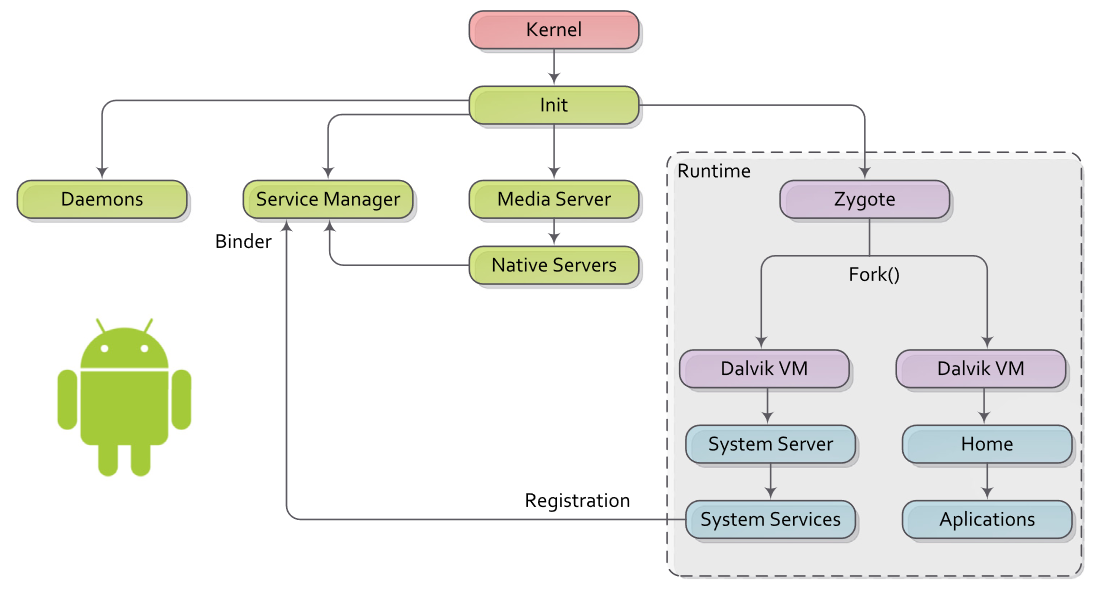
\includegraphics[width=\linewidth]{bootsq}
	\caption{Android boot sequence \cite{vidal2018}.}
	\label{bootsequence}
\end{figure}

This sandbox application design inherently restricts potentially dangerous functionality if not declared by the app \cite{barrera2010}. The required permissions of an application is declared in the AndroidManifest.xml file, such as to get location services, access contacts, or images. At this point in time, Android had over 110 permissions. The permissions listed in the file are presented at the install-time to the user, who can either accept and continue the installation or deny, which halts the installation. Permissions are divided into normal and dangerous, where normal permissions are hidden from the user until they wish to expand the total list of permissions the app requires.
 
\section{Post-2015 Era}
As of Android 6.0 (API level 23), Google introduced runtime permissions and special permissions in addition to the install-time permissions \cite{devAndroid}. 

\subsection{Install-time permissions}
Install-time permissions enable applications to access restricted data and allow them to perform limited actions that may have a marginal effect on other system or third-party apps. When the developer declares install-time permissions, they are displayed on the app store, and automatically granted when the user installs the app. Sub-types of install-time permissions include normal permissions and signature permissions.

\textbf{\sffamily Normal permissions}\\
These include data and actions that extend beyond the app's sandbox. They are classified as normal protection levels because they present little to no risk to user's privacy and the operation of other apps. 

\textbf{\sffamily Signature permissions}\\
A permission that the system grants only if the requesting application is signed with the same certificate as the application that declared the permission. Therefore, if an app declares a signature permission that another app has defined, and both applications are signed by the same certificate, the system grants the permission to the first app after installation without the user's explicit approval. Otherwise, the permission will not be provided to the first app. While the definition of install-time permissions states that the overall impact is marginal to the system and the other apps, signature permissions somewhat defy this interpretation. However, since the access given to the app by this type of permission is bound on a certificate, a developer can only give access to a secondary application that is built by them. The meaning is that the type of access enabled is not marginal, however, the scope is reduced so much that the effect on the user is naught. An app with signature permissions has only so much access that the user already consented to give to the developer. Therefore, signature permissions enable the developer to provide a convenience for the user at no cost to their privacy.

\subsection{Runtime permissions}
Known as the dangerous permissions before Android 6.0, runtime permissions give applications additional access to restricted data that can have a significant effect on the system and other third-party apps. As opposed to install-time permissions, declaring these permissions result in a permission prompt during runtime. They can access personally identifiable information of the user. Hence, these permissions have their protection levels classified as dangerous.

\subsection{Special permissions}
These permissions are defined by the platform and OEMs to carry out specific app functionalities. In addition, the platform and OEMs can define special permissions in order to restrict or protect access to dangerous actions. Special permissions are classified as the \textit{appop} protection level. These are basically signature permissions for manufacturers and platform developers, hence the designation \texttt{signature|appop}.

\subsection{Alternatives to permissions}
As seen in Figure \ref{workflow}, modern Android documentation urges application developers to declare permissions only in situations where alternatives are not available. Asking the user for a postal code or an address instead of declaring \texttt{ACCESS\_COARSE\_LOCATION} permission is suggested. Another example is the app using the system camera app, where it is encouraged to invoke \texttt{ACTION\_IMAGE\_CAPTURE}, or \texttt{ACTION\_VIDEO\_CAPTURE} instead of declaring the \texttt{CAMERA} permission. In the situations where the app needs to access content that another app has created, it is stated that instead of declaring \texttt{READ\_EXTERNAL\_STORAGE} permission, it is better to use the smartphone media store to open media files, and Storage Access Framework to open other files and miscellaneous documents. Media store is a framework that provides an index to media collections, allowing for retrieving and updating media files. Storage Access Framework has similar functionality for non-media content.
\begin{figure}\centering
	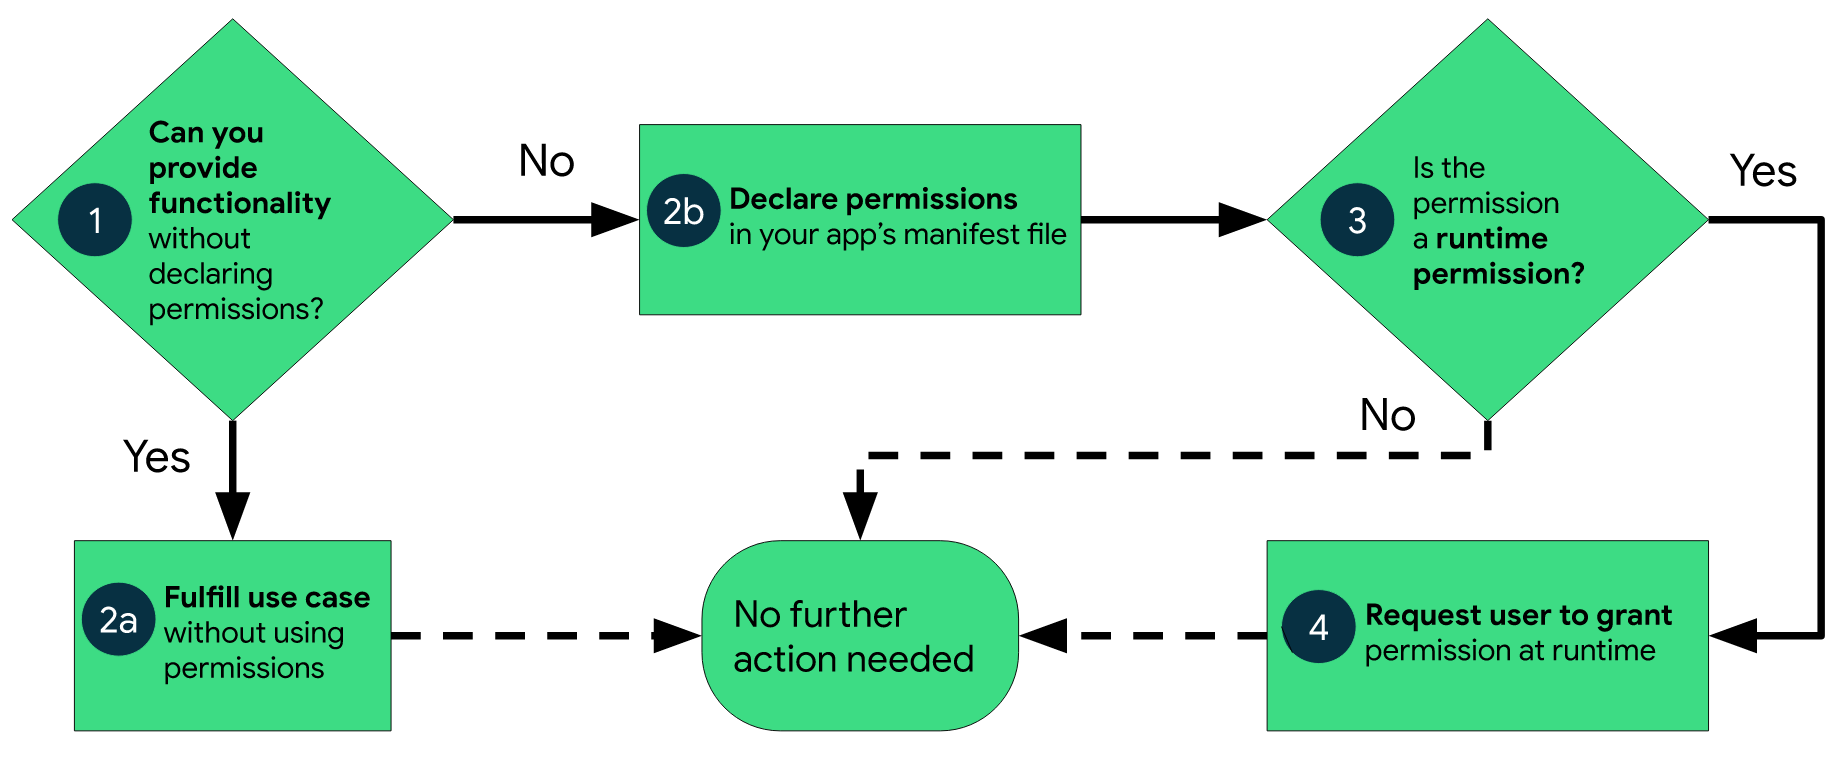
\includegraphics[width=\linewidth]{permworkflow}
	\caption{High-level workflow for using permissions on Android \cite{devAndroid}.}
	\label{workflow}
\end{figure} 
Documentation indicates that as of Android 10 (API level 29), accessing the device IMEI is not possible. If the application requires identification of the device for whatever purpose, it needs to get a unique device identifier for specific app's instance using the Instance ID library. In the case of pairing a device over Bluetooth, using companion device pairing instead of declaring \texttt{BLUETOOTH\_ADMIN}, and \texttt{ACCESS\_FINE\_LOCATION} permissions is recommended. Companion device pairing is a service for devices running on Android 8.0 (API level 26) and higher, that allows for Bluetooth or Wi-Fi scan of nearby devices. Barrera et al. had noted that in the previous Android versions, it was difficult to find a balance between finer and coarser-grained permissions. This issue will further be discussed in the literature review section.

\subsection{Custom App Permissions}
In an effort to further protect Inter-Process Communication (ICP), Android also introduced custom permissions \cite{customAndroid}. Apps can make their functionality available to other apps by defining new permissions that can be requested, in addition to defining automatically granted applications that share the same signature.

\chapter{Literature Review}
\label{cha:litreview}

In this chapter, existing research is compiled. The prevailing range of issues facing the Android permission scheme that is popular among scholars includes application overprivilege, analysis of app network usage, vulnerability analysis, attacks conducted without any permissions, OS version distribution, and most importantly, changes that came with Android 6.0.

\section{Overprivilege}
According to Wang et al. in a 2013 paper, application overprivilege can be a serious problem in the Android permission scheme \cite{wang2013}. They claim that quite a lot of developers and users are hardly mindful of whether the requested permissions hold any functional purpose. In their analysis, they randomly select 50 apps from the Google Play Store and another third-party store and find that overprivilege is a common problem. Although the results show that the issue is much more severe in the third-party store, the authors found that around 44\% of the apps they tested requested unnecessary permissions.

A study on application overprivilege of 71 educational apps show worrying results \cite{alenezi2017}. Authors claim that depending on the users alone for permissions is was a poor solution for previous issues. In the experiment, they analyze every declared and used permission. Analysis showed that 25\% of the total declared permissions were custom permissions. It was also found that approximately 80\% of the apps declared more permissions than what they actually used. Alenezi et al. suggest an integrated solution that detects discrepancies between declared and used permissions. They believe that even under development, an IDE should display whether the declared permissions are being used or not.

\section{Application analyses}
In 2014, on their analysis of 35 Android applications, Taylor et al. found significant problems regarding network usage of apps \cite{taylor2014}. All but one of the applications sent some amount of data encrypted using SSL, however, 80\% of the apps also sent information in plaintext. Well over half of these apps were responsible for privacy leaks. There is some reasoning behind why encrypted and unencrypted connections were used in combination. It may be due to the scalability issues that came with the SSL at the time, or simply the price of SSL certificates, both reasons resulting in a higher upkeep cost. Attackers can find out the make and model of the device, including the OS version and installed apps. All of this information can lead an attacker to pinpoint specific exploits for particular devices. In addition, attacks on encrypted connections are also possible. Stöber et al. note that although the content is hidden from eavesdroppers, an attacker can gather side-channel information such as timing and data volume through fingerprinting periodic traffic patterns with a high success rate \cite{stoeber2013}. 

Users do not explicitly see the network usage and security configuration of an application. This can lead to data theft, location tracking, or device damage \cite{ferreira2015}. Android Play Store's automated screening process to detect malware is unreliable and can be dodged. Approximately 70\% of the network traffic generated by a device is unseen by the user. Android users can check the volume of the traffic, but the exact time and destination data is not easily available. It is difficult for a user to discern a malicious app that may be generating undesirable or potentially damaging traffic. Furthermore, if an app functions merely in the background, the user has little idea on the purpose of the internet access beyond what the app claims. Ferreira et al. demonstrate that around 56\% of connections set up by third-party apps were on insecure ports. In addition, as Taylor et al. also mention, even the secure SSL connections are used widely incorrectly. Incorrect implementation of SSL can lead to passive eavesdropping attacks.

A 2014 paper from Fang et al. highlights the issues that come with the permission-based security of Android, such as coarse-granularity of permissions, the difficulty of permission administration, lack of adequate documentation, overprivilege, etc \cite{fang2014}. As shown in Figure \ref{issueRel}, the issue categorization is twofold; direct and indirect issues. Direct issues can cause leakage of private information, or monetary damage, while indirect issues may be utilized as a vehicle in an attack scenario.
\begin{figure}\centering
	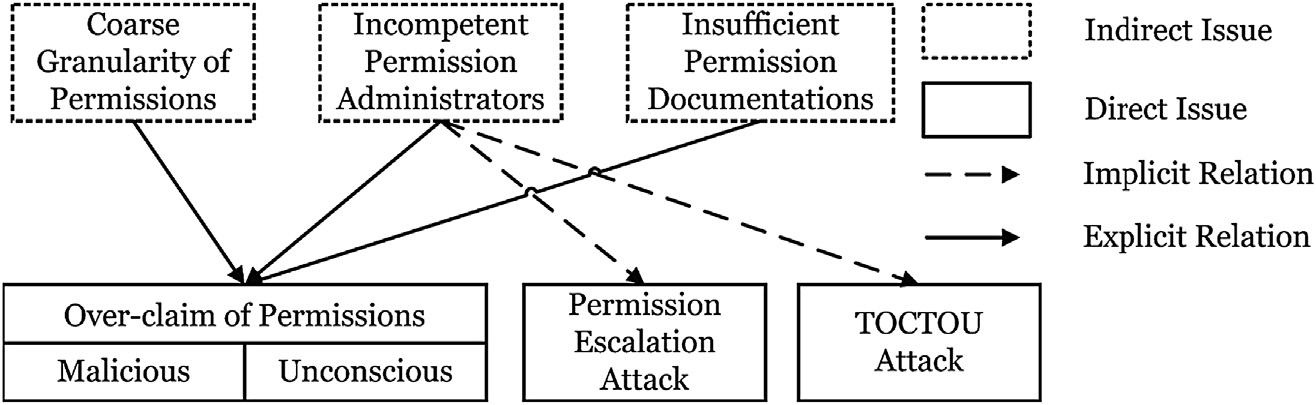
\includegraphics[width=\linewidth]{issueRel}
	\caption{Relationship between issues in Android permission scheme \cite{fang2014}.}
	\label{issueRel}
\end{figure} 
Direct issues include overprivilege, permission escalation attack, and TOCTOU (Time of Check to Time of Use) attack. Indirect issues include coarse granularity, incompetent permission administration, and lack of documentation. It is known that coarse-grained permissions lead to difficulty for users to detect overprivilege. TOCTOU attack refers to some signature permissions granted for another application. Even if the app is uninstalled, the permissions are never revoked, so a new app with the same certificate would have access to the same permissions without approval. Authors cite the \texttt{INTERNET} permission as an example for coarse granularity. A malicious developer might declare this permission to display advertisements in their app, at the same time, they can utilize this permission to access tolled websites secretly.

As it can be seen in Figure \ref{issueRel}, indirect issues can be implicitly or explicitly related to direct issues. Many permissions of this era give arbitrary access to device resources. It gives way for malicious apps to put on a mask of legitimacy. Manifest files are written by developers for requesting permissions. When this file is being written, the developer may or may not know in detail what kind of risks they entail. Some developers may take their time to educate themselves on the capabilities of these permissions, while others may simply claim them to make sure their app works. 
%can add more from fang paper as needed, direct categorized text available, at least one or two pages 

\section{Vulnerability analysis}
Huang et al. conduct a general trend analysis to demonstrate the situation in the Android mobile vulnerability market \cite{huang2015}. An evaluation of a known vulnerability is conducted by taking note of the disclosure date of each CVE vulnerability and calculating the disclosed vulnerabilities year by year since 2008. In addition, all vulnerabilities disclosed in NVD are also retrieved to estimate the percentage of vulnerabilities per year. It is observed from Figure \ref{vuln-disc} that vulnerabilities related to Android increased from 2008 to 2012. Following a small decline in 2013, there was an outbreak of vulnerabilities in 2014.
\begin{figure}\centering
	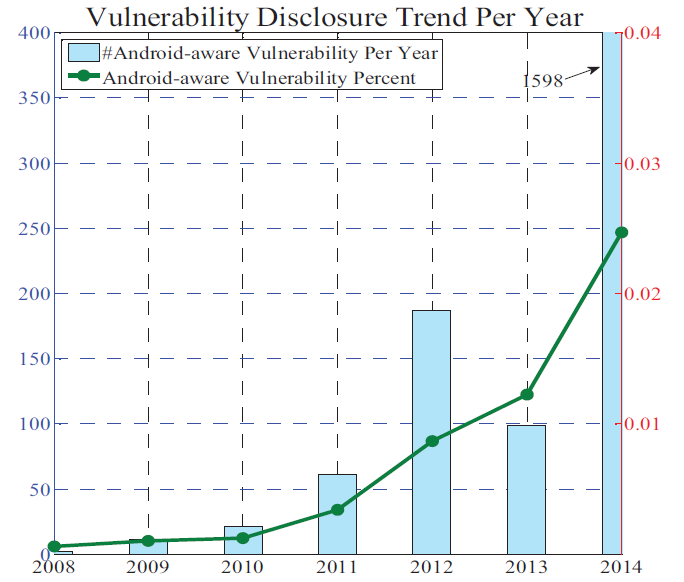
\includegraphics[width=11cm]{vulnDisclosure}
	\caption{Vulnerability Disclosure Trend Per Year \cite{huang2015}.}
	\label{vuln-disc}
\end{figure}
The sharp escalation in 2014 is due to the fact that several Android software products could not validate SSL certificates given by HTTPS connections. Overall, the authors conclude that the security of the Android ecosystem has worsened over time. They divide the evolution of vulnerability market in three periods: period A (2008-2010) where the majority of vulnerabilities are functional, period B (2009-2013) where the market is still dominated by functional vulnerabilities, however, management vulnerabilities arise (permission, privileges, and access control), and lastly, period C (2014-2015) where management vulnerabilities such as CWE264 and CWE310 prevail.

Huang et al. analyze vulnerability severity pattern by comparing all vulnerabilities in the software industry to relevant Android vulnerabilities. They find that the average risk score for the Android market is greater than the industry for the most part. The average CVSS risk score for the Android market is over 7, which can be considered as high risk, while the score for the industry is between 6 and 7, which makes it medium risk. The software market vulnerabilities are decreasing over time. Furthermore, the percentage of high-risk vulnerabilities to others is considerably higher to that of whole market. Therefore, one can state that the Android market's security is worse than the whole software industry market.

CVSS includes an exploitability sub-score which indicates a vulnerability's likelihood to be exploited in terms of access vector, access complexity and authentication. It is noted that remotely exploitable vulnerabilities for the industry is approximately 90\% with a slight decrease over the years, while the Android market's remotely exploitable vulnerabilities have an upwards trend and more than 90\%. Access complexity is seen to be increasing, meaning that more sophisticated methods are required for exploitation, while the opposite is true for the Android market. Across the entire industry, the percentage of exploitable vulnerabilities without authentication is dropping. The overwhelming majority of the Android market vulnerabilities can be exploited without requiring authentication. As a result, the vulnerabilities in the Android market are more exploitable and easier to exploit over time than the vulnerabilities in the entire market. Strengthening the authentication process is the most effective approach for securing the Android market.

CVSS impact subscore assesses the adverse effects to a system if the vulnerability is successfully exploited. The confidentiality impact refers to the scope that attackers can access, integrity impact refers to what the attackers can alter, and availability impact refers to how attackers can affect the accessibility of system resources. Most vulnerabilities in the Android market have a complete confidentiality, integrity and avaiability impact. Hence, the impact score for the Android market is higher than the entire market.

Authors conclude that number of vulnerabilities in the Android market is higher, and they are more exploitable. While the entire market is seeing an improvement, the security situation in the Android market has been declining until 2015 in which the year this vulnerability analysis study was written. 

\section{Attacks without permissions}
Kywe et al. demonstrate that even without any permissions, an attacker can gain access to device ID, phone service state, SIM card state, Wi-Fi and network information, and user configuration information \cite{kywe2016}. First, they analyze unprotected APIs, which permit third-party apps to interact with device resources without permissions. Following this, they exhibit various attacks using unprotected APIs. A rigorous process is required for retrieving unprotected APIs. Three types of static source-code analysis is performed to achieve this. A call graph analysis on system services to discover permissions without Linux ID checking and permission checking mechanisms on Android Interface Definition Language (AIDL); a component analysis on system applications for identification of unprotected broadcast receivers, services, and activities; a data-flow analysis for locating dynamically registered broadcasts. The analysis is implemented on Android Open Source Project (AOSP) version 5.1.0\_rl and 4.4.0\_rl. They find 735 unprotected APIs in system services for version 5.1.0\_rl. The more recent version contains more unprotected APIs than the 4.4.0\_rl due to additional functionalities added.

Following the discovery of unprotected APIs, Kywe et al. develop a third-party application that conducts Java reflection attacks, broadcast injection attacks, broadcast hijacking attacks, malicious activity launch attacks, activity hijacking attacks, malicious service launch attacks, and service hijacking attacks without requesting any permissions. The findings show that on version 4.4.0\_r1, the malicious app can block email synchronization, calendar events, and alter device settings, browser settings, Google documents. On version 5.1.0\_r1, the malicious app can see private user information such as country, Wi-Fi details, Bluetooth, cell signal strength, NFC, power state, SIM card state, and device ID strength. An attacker can control the volume of Android phones and play the ringtones, alarms, and notification tones that users have configured for calls and texts. Even if the target devices are secured, an attacker can disable Bluetooth discovery services and access camera, mail, music, and other device applications.

\section{OS version distribution}
In the iOS market, there exist no manufacturer variables. iOS devices are supported for seven years after the last time Apple sold that specific model. Over 80\% of the devices with iOS in the market have the latest OS version installed \cite{appleStat}. From a security perspective, it is a good practice to use the latest OS version in a device, however, this is not a reality for the Android market. The distribution of Android OS versions in the market is affected by variables such as a large number of different types of devices and numerous manufacturers who sell these devices. On average, an Android smartphone is supported for two to three years.
\begin{figure}\centering
	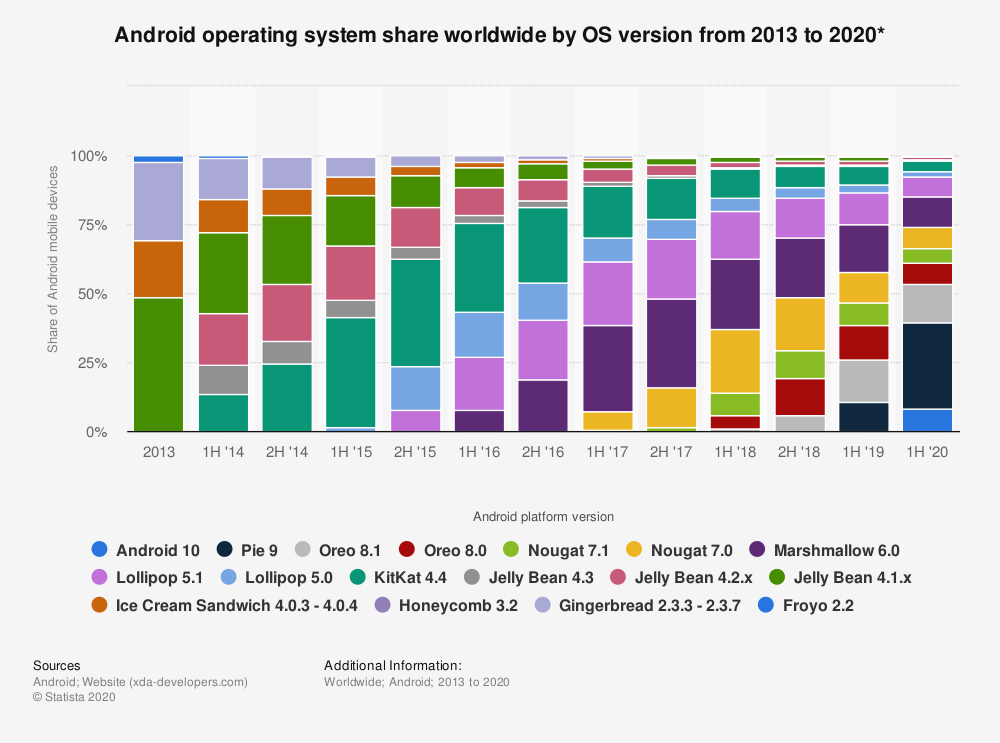
\includegraphics[width=13cm]{androidstat}
	\caption{Android OS version distribution in the worldwide market \cite{androidStat}.}
	\label{andstat}
\end{figure}
This results in a considerable number of devices with outdated and unsupported versions being actively used in the market \cite{androidStat}. Figure \ref{andstat} demonstrates that approximately 60\% of the devices are running on an Android OS that is over two years old. Despite being six years old, Android 6.0 was the second most widely used version in 2020. Over 15\% of the devices are being run with OS versions between 4.0 and 5.1. In a market with well over two billion smartphones, these percentages are worrying to say the least.  

\section{Changes with Android 6.0}
As mentioned before, after Android 6.0, the permissions were divided into install-time and runtime permissions. Normal and signature permissions were granted during install, while dangerous permissions were granted at runtime, with the option given to the user to revoke them at any time. These runtime permissions were divided into groups such as the one shown in Figure \ref{permgroups}. 
\begin{figure}\centering
	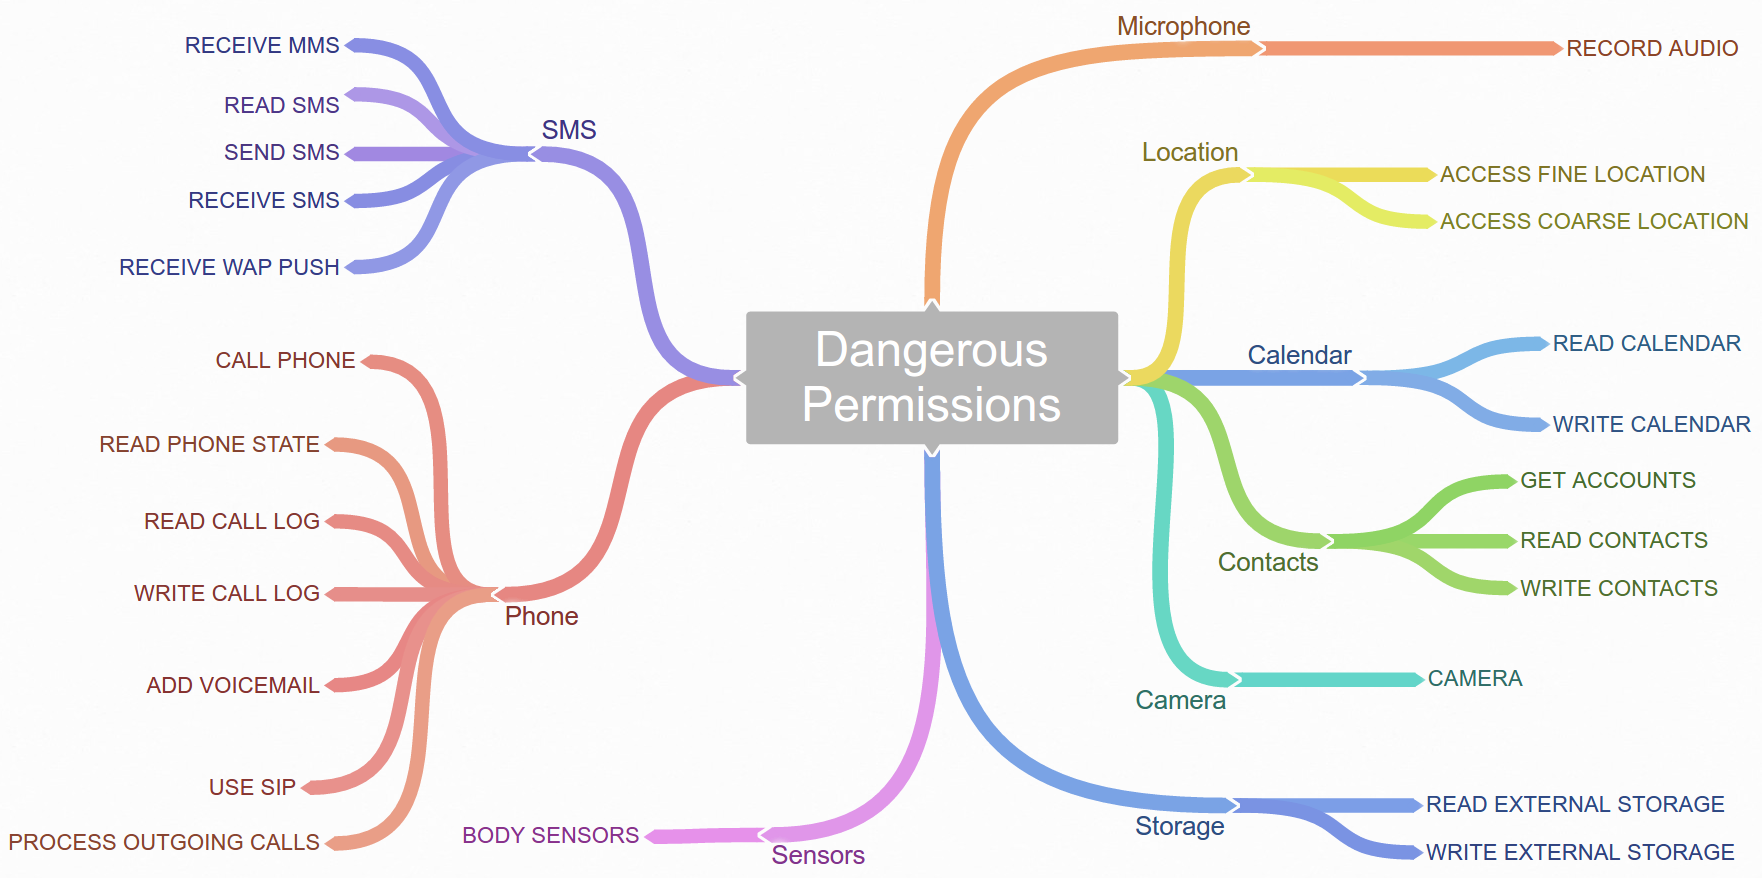
\includegraphics[width=\linewidth]{permgroups}
	\caption{Groups for dangerous permissions \cite{alepis2017}.}
	\label{permgroups}
\end{figure}
Special protected API calls were introduced to \texttt{PackageManager} to provide runtime permissions, allowing users to grant and remove access dynamically. New APIs were also added, allowing app developers to check if permissions are granted at runtime and, if necessary, request them. If one permission from a group was granted to an application, the other permissions in that group were granted to that app as well. Zhauniarovich et al. claim that Android 6.0 has undergone a change for the worse, where a more coarse-grained structure is implemented rather than the opposite \cite{zhauniarovich2016}. In the previous versions, apps with the same digital signature as the package declaring the permission were granted signature permissions at install time. However, Android has introduced various new kinds of signature permissions that can be requested by third-party apps that do not meet this requirement. Moreover, 22 permissions that were previously regarded as dangerous are now granted at install time, with no way to revoke them by the user. Permissions such as \texttt{BLUETOOTH}, \texttt{NFC} and \texttt{INTERNET} need not be approved by the user anymore.

Since many devices in use were running previous versions of Android, new apps had to be forward compatible with older versions. Google's new special compatibility library included the API calls for checking granted permissions. Authors discovered that if the app is running on an older version of Android that hasn't yet declared the permission, API call from special compatibility library returns \textit{denied} for some permissions that are not even required in the first place. Since older versions of Android are hardly supported, it is highly difficult to apply a fix to the problem. Authors suggest that it should at least be noted in the documentation, so the developers can look out for it.

The AppOps system allows users to give and revoke permissions at runtime through a dedicated user interface within the Settings, allowing old apps to work with the new version of Android for backwards compatibility. AppOps, on the other hand, solely manages platform permissions and so is unable to enforce developer-defined custom dangerous permissions. When a legacy app is installed on a device, the user is indeed prompted with the pre-6.0 type of permission alert box. If the user does not consent to the prompted permissions, the app will not be installed. The intention was to make legacy and new apps behave in the same manner, but that did not happen according to Zhauniarovich et al. Backwards compatibility also opened a way for malicious app developers to take advantage of post-Marshmallow OS versions, specifically creating apps that do not traverse beyond API Level 23, so that their apps do not hold any runtime permissions, and all their dangerous permissions accepted at install-time \cite{alepis2017}. Since the user is accustomed to the new permission system, initially accepting what the app asks might not seem as dangerous. 

Zhauniarovich et al. take issue with runtime permissions being granted per permission groups. They claim that while this reduces the number of interruptions a user receives during runtime, however, users who want to have a finer-grained permission control on their devices are not being considered. Alepis et al. also give an example of the problems that come with dangerous permission groups. They consider a use case where an app that requires access to phone functionalities and declares the permission \texttt{READ\_PHONE\_STATE}. The user will be prompted by an alert box stating "Allow the application to make and manage phone calls?". This vague statement will allow the app to read and change the call history, and make phone calls without user notification.  

%exploring permissions post marshmallow alepis 
Alepis et al. also argue that after Android 6.0, transparency of permissions has decreased, and fine-grained control is not being offered, and the new system altogether is not an improvement to the pre-6.0 versions \cite{alepis2017}. The authors also note users are not completely informed of what the app actually holds for the user. Play Store goes as far as stating that the app to be installed does not require special access while in reality, for some cases the opposite is true. The specific timing for asking runtime permissions is problematic as well, usually asking just after the first launch of an app, instead of asking at a time when the app needs access. Another transparency issue comes with apps that only ask for normal (install-time) permissions. In a case where an app asks for both dangerous and normal permissions, users are able to see both types of permissions in the Settings app. However, if an app only declares normal permissions in its Manifest file, users cannot see any permissions in the Settings app, this capability is not enabled. This might lead to some serious security problems, such as an app declaring absolutely no permissions at install-time, and then adding an arbitrary number of normal permissions with updates, leaving the user without any control for the matter.



%yet to include: custom perms, automatically granted perms
%attacks such as session fingerprinting and location tracking may be
%better suited for experiment results and such

\chapter{Methodology}
\label{cha:methodology}
The research methodology includes an extensive literature review located in \cref{cha:litreview}. The experimentation is carried out with two devices, of which the specification is explained in Section 4.1. For the first part of the investigation, two applications are built using Android Studio IDE using Java programming language. Section 4.2 gives an overview of the applications. The second part of the investigation consists of rooting the devices, and noting the differences between the retrievable information, in addition to attempting to provide the apps with superuser privileges. The experimentation is conducted with a focus on the confidentiality principle of information security. The findings are analyzed in \cref{cha:discussion}. Comparisons are drawn based on the differences across devices and applications.   

\section{Test Device Specification}
In order to conduct the experiment, two smartphones of which one employing older and one newer OS version, were acquired. The older device is an HTC One SV, which is equipped with an Android version 4.2.2 (API level 17). The newer device is a BQ Aquaris X Pro, which has the 8.1.0 version (API level  27) of Android. Device information for both smartphones can be seen in Figure \ref{devinf}. These two devices cover the version discrepancy of the Android devices in the market, enabling us to get a broad idea on both sides of the coin.
\begin{figure}\centering
	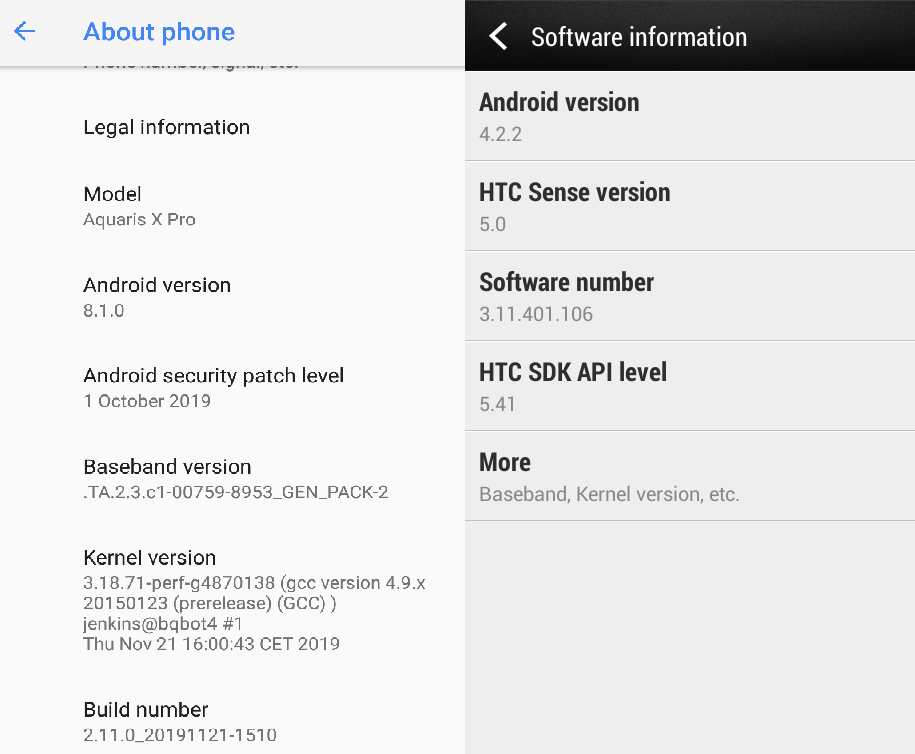
\includegraphics[width=11cm]{deviceinf}
	\caption{Device information pages for the two smartphones (left: BQ Aquaris X Pro, right: HTC One SV).}
	\label{devinf}
\end{figure} 

\section{Application Overview}
Since the app does not have any functionality for the user, it is built upon an empty project template from the Android Studio IDE. The app differs with respect to the permission declaration, where one would have to request permissions in the BQ device during runtime, as opposed to the app for the HTC device, where all the permissions are requested during install-time. 

The Android Studio project folders which include every code and manifest file can be found in the following GitHub link:

\begin{itemize}
	\item https://github.com/erdemcagri/masterthesis-androidstd/
\end{itemize}

\subsection{Application for the BQ device}
The first app to be built was for the BQ device. It was previously mentioned that the app would have two states, one state with all permissions requested from the user, and another state with zero declared permissions.

For the first state with all permissions declared, the initial action was to list all permissions in alphabetical order using the completion assist in Android Studio. This resulted in a grand total of 169 permissions declared in the \texttt{AndroidManifest.xml} file. However, Android Studio immediately flagged a considerable number of these permissions for various reasons such as being deprecated or being reserved for the system applications. Of all the permissions listed, 89 were shown as reserved for the Android system; or they were signature permissions, thus commented out of the manifest file. Nine of the permissions listed were seen as deprecated. Seven of these permissions were commented out except for \texttt{PROCESS\_OUTGOING\_CALLS} and \texttt{USE\_FINGERPRINT} because these two were deprecated later, and were valid for API level 27. The remaining 73 permissions were categorized as install-time or runtime because this distinction makes it easy to see which permissions need to be actually requested from the user. Since the app was configured to work with devices up to API level 27, the runtime permissions that were added after this level were also commented out. These include one API level 28 permission, namely \texttt{ACCEPT\_HANDOVER}, and three API level 29 permissions, which are \texttt{ACCESS\_BACKGROUND\_LOCATION}, \texttt{ACCESS\_MEDIA\_LOCATION}, and \texttt{ACTIVITY\_RECOGNITION}. The final number of runtime permissions was 27, while 42 permissions were listed under the install-time category. Lastly, runtime permissions were divided to their nine specified permission groups. These permissions can be seen in the Table \ref{appbqfperms}.

\begin{table}
\centering
\begin{tabular}{ |p{2.4cm}||p{4cm}|  }
\hline
\multicolumn{2}{|c|}{Runtime Permissions} \\
\hline
Permission Groups & Permissions\\
\hline\hline
CONTACTS & \texttt{GET\_ACCOUNTS} \\
& \texttt{READ\_CONTACTS} \\
& \texttt{WRITE\_CONTACTS} \\
\hline
CALENDAR & \texttt{READ\_CALENDAR} \\
& \texttt{WRITE\_CALENDAR} \\
\hline
SMS & \texttt{SEND\_SMS} \\
& \texttt{RECEIVE\_SMS} \\
& \texttt{READ\_SMS} \\
& \texttt{RECEIVE\_WAP\_PUSH} \\
& \texttt{RECEIVE\_MMS} \\
\hline
STORAGE & \texttt{READ\_EXTERNAL\_STORAGE} \\
& \texttt{WRITE\_EXTERNAL\_STORAGE} \\
\hline
LOCATION & \texttt{ACCESS\_FINE\_LOCATION} \\
& \texttt{ACCESS\_COARSE\_LOCATION} \\
\hline
PHONE & \texttt{READ\_PHONE\_STATE} \\
& \texttt{READ\_PHONE\_NUMBERS} \\
& \texttt{CALL\_PHONE} \\
& \texttt{READ\_CALL\_LOG} \\
& \texttt{WRITE\_CALL\_LOG} \\
& \texttt{ADD\_VOICEMAIL} \\
& \texttt{USE\_SIP} \\
& \texttt{PROCESS\_OUTGOING\_CALLS} \\
& \texttt{ANSWER\_PHONE\_CALLS} \\
\hline
MICROPHONE & \texttt{RECORD\_AUDIO} \\
\hline
CAMERA & \texttt{CAMERA} \\
\hline
SENSORS & \texttt{BODY\_SENSORS} \\
& \texttt{USE\_FINGERPRINT} \\
\hline
\end{tabular}
\begin{tabular}{|p{6.5cm}|}
\hline
{Install-time Permissions} \\
\hline\hline
\texttt{ACCESS\_NOTIFICATION\_POLICY} \\
\texttt{ACCESS\_WIFI\_STATE} \\
\texttt{BLUETOOTH} \\
\texttt{BLUETOOTH\_ADMIN} \\
\texttt{BROADCAST\_STICKY} \\
\texttt{CALL\_COMPANION\_APP} \\
\texttt{CHANGE\_NETWORK\_STATE} \\
\texttt{CHANGE\_WIFI\_MULTICAST\_STATE} \\
\texttt{CHANGE\_WIFI\_STATE} \\
\texttt{DISABLE\_KEYGUARD} \\
\texttt{EXPAND\_STATUS\_BAR} \\
\texttt{FOREGROUND\_SERVICE} \\
\texttt{ACCESS\_LOCATION\_EXTRA\_COMMANDS} \\
\texttt{ACCESS\_NETWORK\_STATE} \\
\texttt{GET\_PACKAGE\_SIZE} \\
\texttt{INSTALL\_SHORTCUT} \\
\texttt{INTERNET} \\
\texttt{KILL\_BACKGROUND\_PROCESSES} \\
\texttt{MANAGE\_OWN\_CALLS} \\
\texttt{MODIFY\_AUDIO\_SETTINGS} \\
\texttt{NFC} \\
\texttt{NFC\_PREFERRED\_PAYMENT\_INFO} \\
\texttt{NFC\_TRANSACTION\_EVENT} \\
\texttt{READ\_SYNC\_SETTINGS} \\
\texttt{READ\_SYNC\_STATS} \\
\texttt{RECEIVE\_BOOT\_COMPLETED} \\
\texttt{REORDER\_TASKS} \\
\texttt{REQUEST\_COMPANION\_RUN\_IN\_BACKGROUND} \\
\texttt{REQUEST\_COMPANION\_USE\_DATA} \\
\qquad\qquad\texttt{\_IN\_BACKGROUND} \\
\texttt{REQUEST\_DELETE\_PACKAGES} \\
\texttt{REQUEST\_IGNORE\_BATTERY\_OPTIMIZATIONS} \\
\texttt{REQUEST\_PASSWORD\_COMPLEXITY} \\
\texttt{SET\_ALARM} \\
\texttt{SET\_WALLPAPER} \\
\texttt{SET\_WALLPAPER\_HINTS} \\
\texttt{TRANSMIT\_IR} \\
\texttt{UNINSTALL\_SHORTCUT} \\
\texttt{USE\_BIOMETRIC} \\
\texttt{USE\_FULL\_SCREEN\_INTENT} \\
\texttt{VIBRATE} \\
\texttt{WAKE\_LOCK} \\
\texttt{WRITE\_SYNC\_SETTINGS} \\
\hline
\end{tabular}
\caption{Declared permissions in AppBQ\_full application}
\label{appbqfperms}
\end{table}

Following the declaration of permissions in the \texttt{AndroidManifest.xml} file, a permission request button was created \cite{permButton}. Next, the code was expanded to request all declared permissions with that one button. In this version of Android, even if one declares runtime permissions in the manifest file, the app will behave as if no permissions are required at install unless they are specifically requested.

The second state of the app is much simpler, which only includes creating a basic application out of an empty template. Alepis et al.'s extensive 2017 study mentioned if the app only declares normal permissions in its manifest file, the user would not be notified and would not be able to see what normal permissions were declared in Settings. Therefore, the app contains no runtime permissions, but all install-time permissions. This notion is further explained in Section 5.2.
\newpage
\subsection{The application for the HTC device}
The creation of the HTC app for the full permissions state was fairly similar to that of the BQ app. Using the Android documentation \cite{perms442}, a categorized list of all permissions were written into the \texttt{AndroidManifest.xml} file. In total, there were approximately 200 permissions listed in the file. 70 permissions under 25 different categories were declared, while the remaining ones were flagged as signature, or as reserved for system applications. Of all the declared permissions, 46 were classified as dangerous protection level, while 24 of them as normal protection level. The full list of permissions can be seen in Table \ref{apphtcfperms}.

\begin{longtable}{|p{5cm}|p{6cm}|p{1.7cm}|}
	\hline
	\multicolumn{3}{|c|}{Declared Permissions} \\
	\hline
	Permission Groups & Permissions & Protection Level\\
	\hline\hline
	MESSAGES & \texttt{SEND\_SMS} & dangerous \\
	& \texttt{RECEIVE\_SMS} & dangerous \\
	& \texttt{RECEIVE\_MMS} & dangerous \\
	& \texttt{READ\_SMS} & dangerous \\
	& \texttt{WRITE\_SMS} & dangerous \\
	& \texttt{RECEIVE\_WAP\_PUSH} & dangerous \\
	\hline
	SOCIAL\_INFO & \texttt{READ\_CONTACTS} & dangerous \\
	& \texttt{WRITE\_CONTACTS} & dangerous \\
	& \texttt{READ\_CALL\_LOG} & dangerous \\
	& \texttt{WRITE\_CALL\_LOG} & dangerous \\
	& \texttt{READ\_SOCIAL\_STREAM} & dangerous \\
	& \texttt{WRITE\_SOCIAL\_STREAM} & dangerous \\
	\hline
	PERSONAL\_INFO & \texttt{READ\_PROFILE} & dangerous \\
	& \texttt{WRITE\_PROFILE} & dangerous \\
	\hline
	CALENDAR & \texttt{READ\_CALENDAR} & dangerous \\
	& \texttt{WRITE\_CALENDAR} & dangerous \\
	\hline
	USER\_DICTIONARY & \texttt{READ\_USER\_DICTIONARY} & dangerous \\
	& \texttt{WRITE\_USER\_DICTIONARY} & normal \\
	\hline
	BOOKMARKS & \texttt{READ\_HISTORY\_BOOKMARKS} & dangerous \\
	& \texttt{WRITE\_HISTORY\_BOOKMARKS} & dangerous \\
	\hline
	DEVICE\_ALARMS & \texttt{SET\_ALARM} & normal \\
	\hline
	VOICEMAIL & \texttt{ADD\_VOICEMAIL} & dangerous \\
	\hline
	LOCATION & \texttt{ACCESS\_FINE\_LOCATION} & dangerous \\
	& \texttt{ACCESS\_COARSE\_LOCATION} & dangerous \\
	& \texttt{ACCESS\_LOCATION\_EXTRA\_COMMANDS} & normal \\
	\hline
	NETWORK & \texttt{INTERNET} & dangerous \\
	& \texttt{ACCESS\_NETWORK\_STATE} & normal \\
	& \texttt{ACCESS\_WIFI\_STATE} & normal \\
	& \texttt{CHANGE\_WIFI\_STATE} & dangerous \\
	\hline
	BLUETOOTH\_NETWORK & \texttt{BLUETOOTH} & dangerous \\
	& \texttt{BLUETOOTH\_ADMIN} & dangerous \\
	& \texttt{NFC} & dangerous \\
	\hline
	ACCOUNTS & \texttt{GET\_ACCOUNTS} & normal \\
	& \texttt{AUTHENTICATE\_ACCOUNTS} & dangerous \\
	& \texttt{USE\_CREDENTIALS} & dangerous \\
	& \texttt{MANAGE\_ACCOUNTS} & dangerous \\
	\hline
	AFFECTS\_BATTERY & \texttt{CHANGE\_WIFI\_MULTICAST\_STATE} & dangerous \\
	& \texttt{VIBRATE} & normal \\
	& \texttt{FLASHLIGHT} & normal\\
	& \texttt{WAKE\_LOCK} & normal \\
	\hline
	AUDIO\_SETTINGS & \texttt{MODIFY\_AUDIO\_SETTINGS} & normal \\
	\hline
	MICROPHONE & \texttt{RECORD\_AUDIO} & dangerous \\
	\hline
	CAMERA & \texttt{CAMERA} & dangerous \\
	\hline
	PHONE\_CALLS & \texttt{PROCESS\_OUTGOING\_CALLS} & dangerous \\
	& \texttt{READ\_PHONE\_STATE} & dangerous \\
	& \texttt{CALL\_PHONE} & dangerous \\
	& \texttt{USE\_SIP} & dangerous \\	
	\hline
	STORAGE & \texttt{READ\_EXTERNAL\_STORAGE} & dangerous \\
	& \texttt{WRITE\_EXTERNAL\_STORAGE} & dangerous \\
	\hline
	SCREENLOCK & \texttt{DISABLE\_KEYGUARD} & dangerous \\
	\hline
	APP\_INFO & \texttt{GET\_TASKS} & dangerous \\
	& \texttt{REORDER\_TASKS} & normal \\
	& \texttt{RESTART\_PACKAGES} & normal \\
	& \texttt{KILL\_BACKGROUND\_PROCESSES} & normal \\
	\hline
	DISPLAY & \texttt{SYSTEM\_ALERT\_WINDOW} & dangerous \\
	\hline
	WALLPAPER & \texttt{SET\_WALLPAPER} & normal \\
	& \texttt{SET\_WALLPAPER\_HINTS} & normal \\
	\hline
	STATUS\_BAR & \texttt{EXPAND\_STATUS\_BAR} & normal \\
	\hline
	SYNC\_SETTINGS & \texttt{READ\_SYNC\_SETTINGS} & normal \\
	& \texttt{WRITE\_SYNC\_SETTINGS} & normal \\
	& \texttt{READ\_SYNC\_STATS} & normal \\
	\hline
	SYSTEM\_TOOLS & \texttt{PERSISTENT\_ACTIVITY} & normal \\ 
	& \texttt{GET\_PACKAGE\_SIZE} & dangerous \\	
	& \texttt{RECEIVE\_BOOT\_COMPLETED} & normal \\
	& \texttt{BROADCAST\_STICKY} & normal \\
	& \texttt{SUBSCRIBED\_FEEDS\_READ} & normal \\
	& \texttt{SUBSCRIBED\_FEEDS\_WRITE} & dangerous \\	
	& \texttt{CHANGE\_NETWORK\_STATE} & dangerous \\	
	\hline
	\caption{Declared permissions in AppHTC\_full application}
	\label{apphtcfperms}
\end{longtable}

For the second state of the app, no permissions were declared. Unlike Android 8.1.0, version 4.2.2 notifies the user at install-time about the declared permissions even if no dangerous permissions were declared. Thus, the manifest file belonging to this state of the application was just an empty project template set at minimum SDK 17.

\chapter{Experiments}
\label{cha:experiments}

It is important to remember the main objective of this thesis. The question to be answered was the leakage of information, such as PII, which is strictly a confidentiality issue. The permissions to be evaluated would be the ones that had a probability of enabling access to a resource that contains information, rather than giving access to alter or remove the data, which means that in other words, security principles aside from confidentiality such as integrity, availability, or non-repudiation is ignored. 

\section{AppBQ\_full}
This is the full permission state of the application for the BQ Aquaris X Pro which is equipped with Android 8.1.0 (API level 27) Oreo OS. In this section, the functionalities of requested runtime permissions will be explored. It will also be tested whether requesting one permission from a permission group enables all permissions in a group. The declared permissions are divided into nine permission groups. These permission groups are contacts, calendar, SMS, storage, location, phone, microphone, and camera.

When the user taps \texttt{AppBQ\_full.apk} to install the app, Android greets them with a message saying "Do you want to install this application? It does not require any special access.". The app has one centered button, stating "REQUEST ALL PERMISSIONS". If the user taps this button, the app then requests all declared permission through nine different prompts for all permission groups These screens can be seen in Figure \ref{oninstall}.
\begin{figure}[H]\centering
	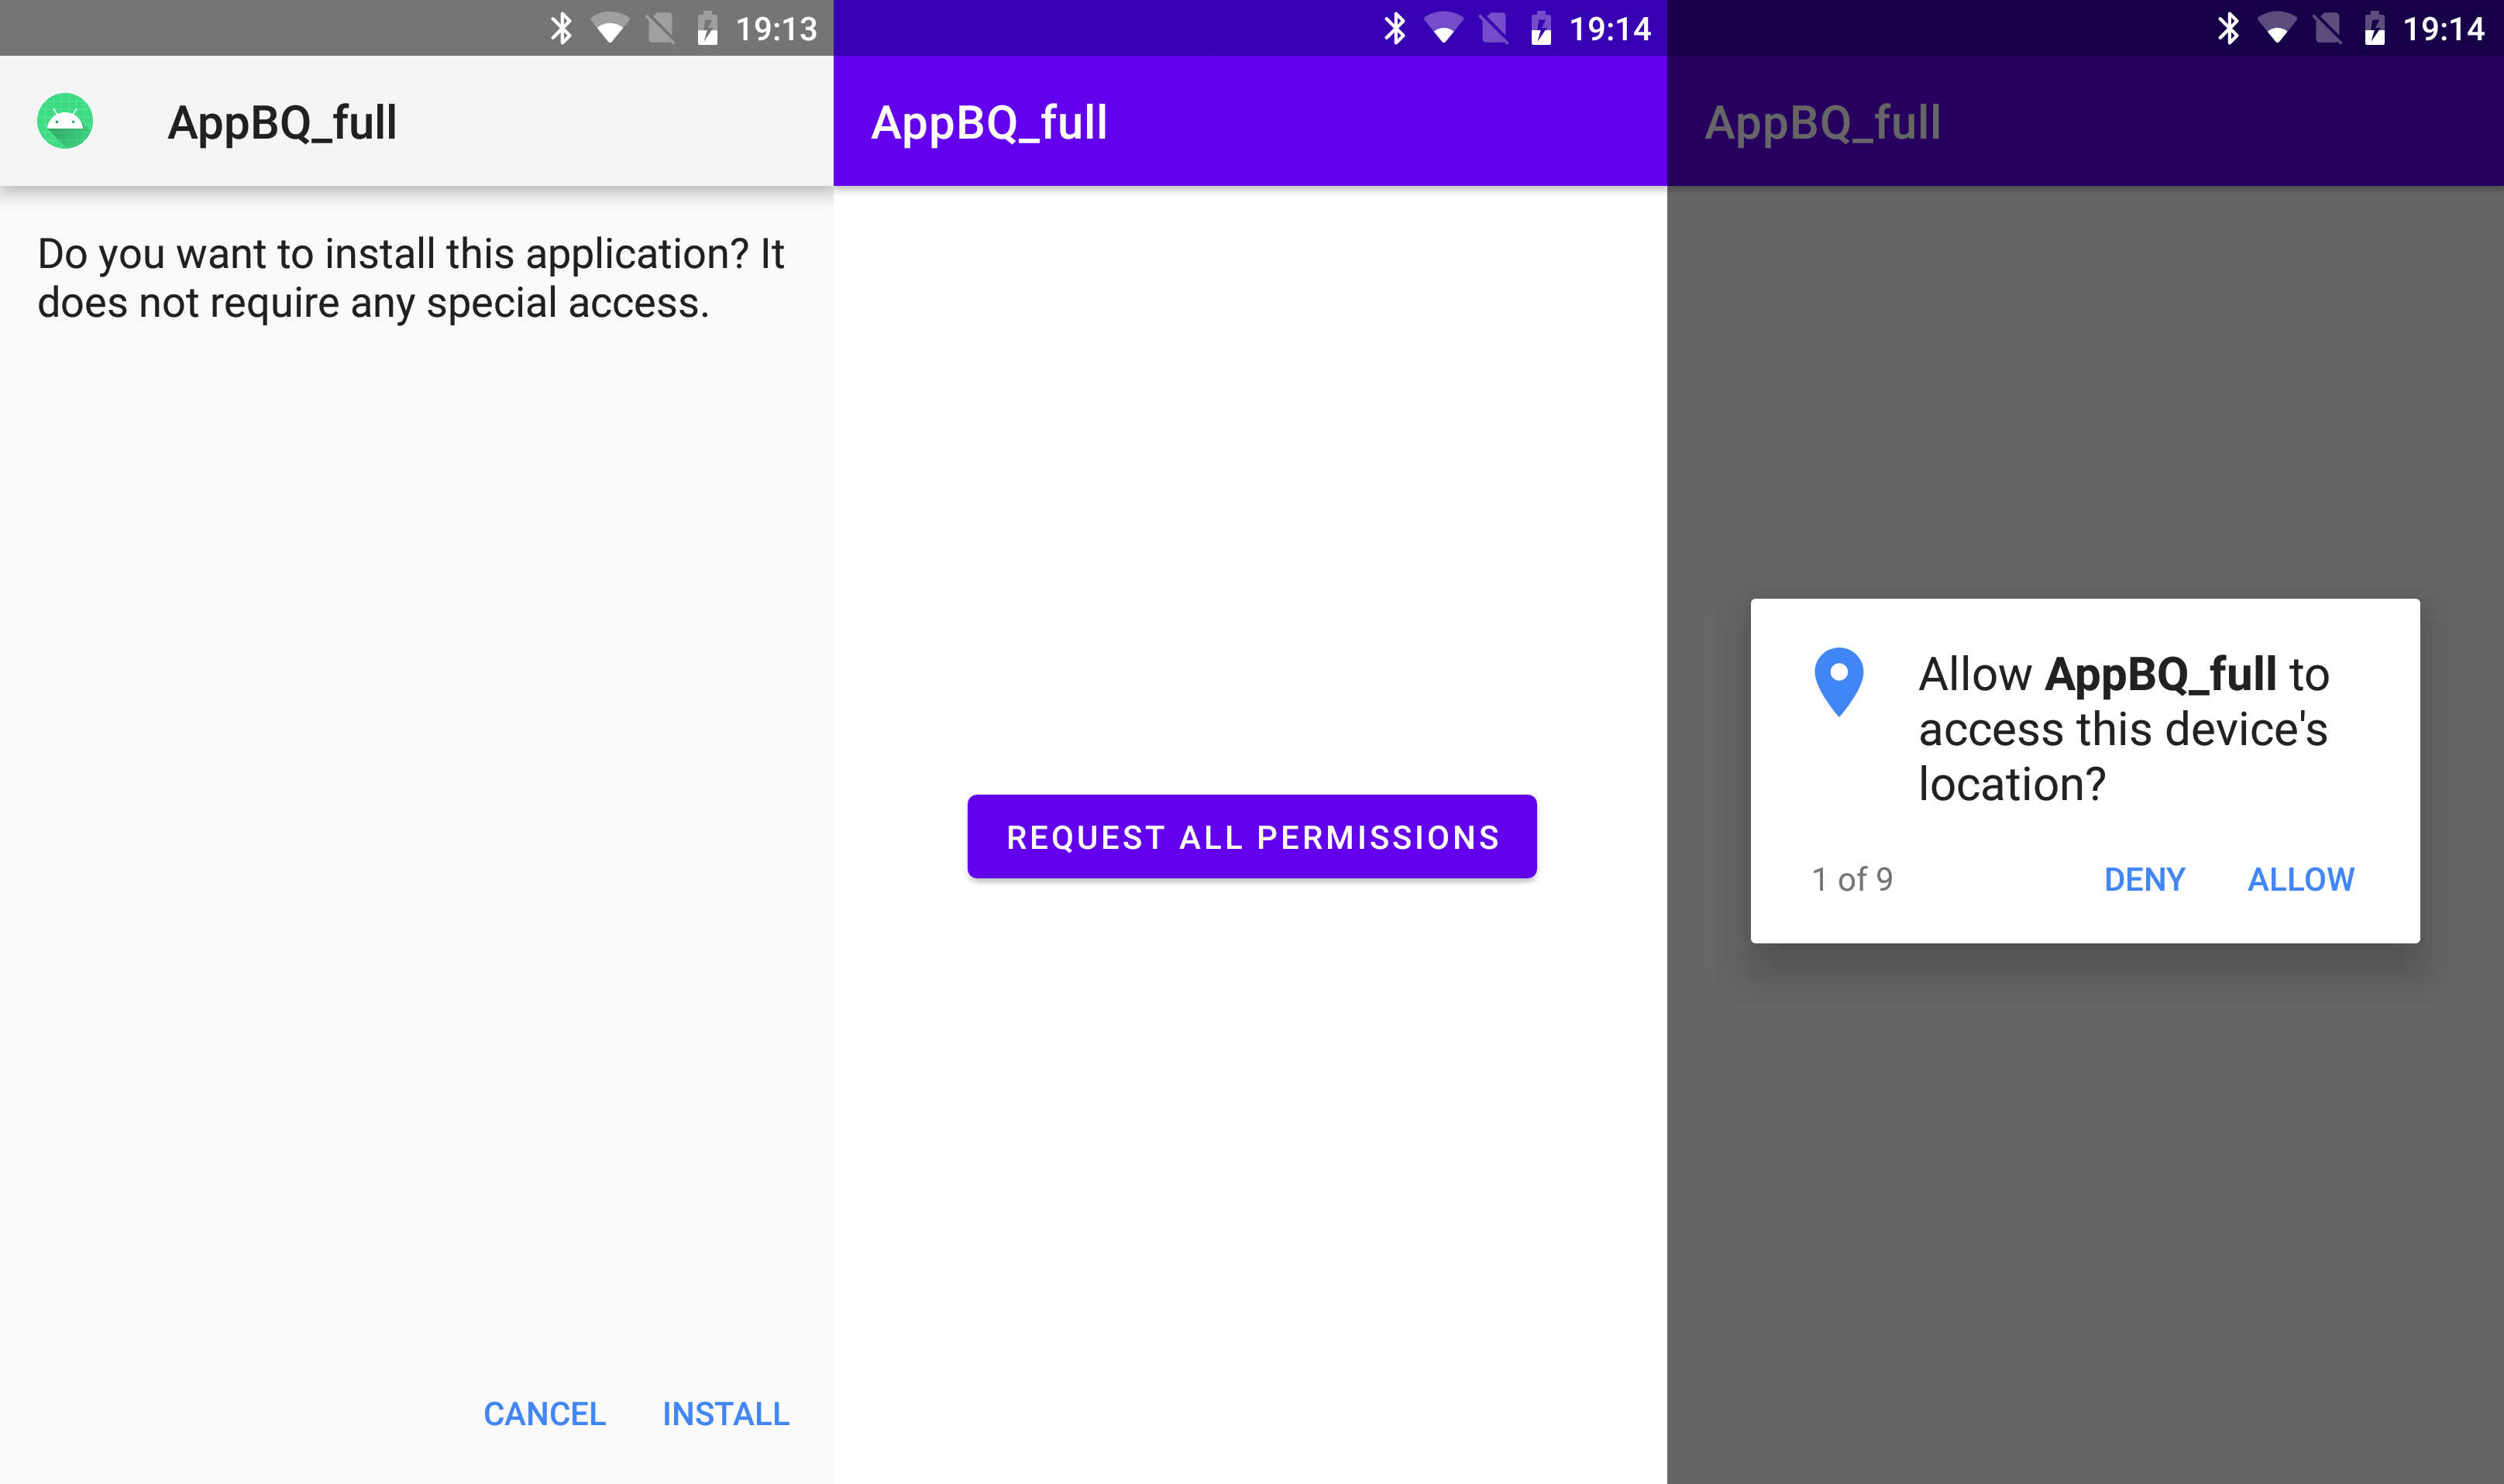
\includegraphics[width=12cm]{oninstall}
	\caption{Screens upon installation of the app with full permissions on BQ Aquaris X Pro.}
	\label{oninstall}
\end{figure} 

\subsection{Permission groups}
In order to store the permission data, a small \texttt{logToFile} method is created, where every time it is called, it appends the data into a text file in the device storage. This method can be seen below.
\begin{lstlisting} 
private void logToFile(Context context, String sBody) {
	File dir = new File(context.getFilesDir(), "permLogs");
	if (!dir.exists()){
		dir.mkdir();
	}
	try {
		File gpxfile = new File(dir, "plogs.txt");
		FileWriter writer = new FileWriter(gpxfile, true);
		writer.append(sBody).append("\n\n");
		writer.flush();
		writer.close();
		Toast.makeText(this, "Data logged to " + context.getFilesDir(), Toast.LENGTH_LONG).show();
	} catch (Exception e) {
		e.printStackTrace();
	}
}
\end{lstlisting}
Using \texttt{context.getFilesDir()}, the \texttt{logToFile()} method creates a "permLogs" folder inside the application path. The method checks if the directory already exists, and if it does, it moves onto creating the text file called "plogs.txt". When the method is called, the \texttt{sBody} string argument is passed to the \texttt{writer.append()} method, so the text in the data stream is appended into the text file. After flushing and closing this stream, a small toast appears in the screen, indicating where the log file is stored.

\subsubsection{Contacts permission group}
The \texttt{android.permission-group.CONTACTS} is used for runtime permissions related to contacts and profiles on a device. Out of the three permissions declared belonging to this group, two are of interest: \texttt{GET\_ACCOUNTS} and \texttt{READ\_CONTACTS}. The \texttt{GET\_ACCOUNTS} permission allows access to the list of accounts in the Accounts Service. 
When the method below is called, it first creates a new \texttt{ArrayList}. Using the \texttt{AccountManager}, every e-mail account in the device is written into the array list, then to the text file using \texttt{logToFile()} method.
\begin{lstlisting}
private String getAcc() {
	List<String> accountList = new ArrayList<String>();
	Pattern gmailPattern = Patterns.EMAIL_ADDRESS;
	Account[] accounts = AccountManager.get(this).getAccounts();
	for (Account account : accounts) {
		if (gmailPattern.matcher(account.name).matches()) {
			accountList.add(account.name);
		}
	}
	return accountList.toString();
}
\end{lstlisting}
This results in a folder creation in the application directory, and a .txt file with the user's e-mail written inside. The e-mail address "testsp.bq@gmail.com" seen in the Figure \ref{grcontacts} was created to demonstrate this permission.
\begin{figure}[H]\centering
	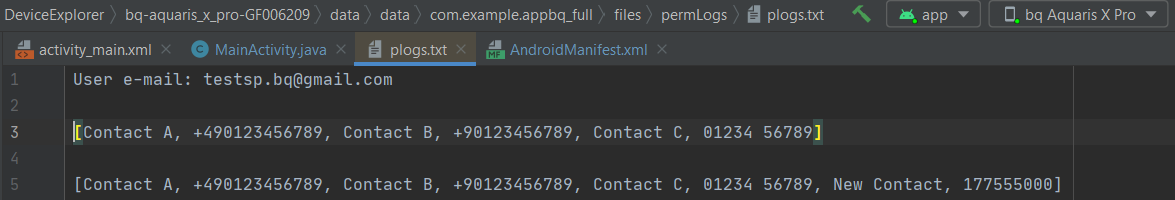
\includegraphics[width=\linewidth]{grcontacts}
	\caption{Text file for the permission log showing user e-mail.}
	\label{grcontacts}
\end{figure}
A similar method was created to write the contacts list in the same "plogs.txt" file using \texttt{READ\_ACCOUNTS} permission. The method \texttt{getContacts()} is a String type method that returns a list of contacts and their phone numbers. \texttt{CurrentResolver} allows the navigation of the contacts database, in which the contact id and phone number is found. After retrieving this data, it is added to the array list \texttt{contactList}, which is also what this method returns after typecasting it to string.
\begin{lstlisting}
private String getContacts() {
	ArrayList<String> contactList = new ArrayList<String>();
	ContentResolver cr = getContentResolver();
	Cursor cur = cr.query(ContactsContract.Contacts.CONTENT_URI, null, null, null, null);
	if ((cur != null ? cur.getCount() : 0) > 0) {
		while (cur != null && cur.moveToNext()) {
			String id = cur.getString(cur.getColumnIndex(ContactsContract
							.Contacts._ID));
			String name = cur.getString(cur.getColumnIndex(ContactsContract
							.Contacts.DISPLAY_NAME));
			contactList.add(name);
			if (cur.getInt(cur.getColumnIndex(ContactsContract
							.Contacts.HAS_PHONE_NUMBER)) > 0) {
				Cursor pCur = cr.query(ContactsContract.CommonDataKinds
								.Phone.CONTENT_URI, null,
				ContactsContract.CommonDataKinds.Phone.CONTACT_ID + " = ?", new String[]{id}, null);
				while (pCur.moveToNext()) {
					String phoneNo = pCur.getString(pCur.getColumnIndex(ContactsContract
									.CommonDataKinds.Phone.NUMBER));
					contactList.add(phoneNo);
				}
				pCur.close();
			}
		}
	}
	if (cur != null) {
		cur.close();
	}
	return contactList.toString();
}
\end{lstlisting}
Only contact names and phone numbers are listed, however, any available contact information can be retrieved such as profile pictures and e-mail addresses. The returned array list can be passed as an argument to the logger method seen before. 

Since the special profile permissions were removed by Android, the \texttt{ContactsContract.Profile} class was also moved to the contacts permission. Thus, I can use the exact same \texttt{getProfile()} method located in AppHTC\_full app, to retrieve the device owner's name and profile ID. The permission entry log relevant to this method can be seen below:
\begin{lstlisting}
[Name: Cagri Erdem - ID: 9223372034707292161]
\end{lstlisting}

\subsubsection{Calendar permission group}
The \texttt{android.permission-group.CALENDAR} is used for runtime permissions related to the user's calendar. \texttt{READ\_CALENDAR}, and \texttt{WRITE\_CALENDAR} permissions were declared from this group. Former permission on reading the calendar information concerns confidentiality, and the method used for this permission is the \texttt{getCalendar()} method. It simply gathers information using the content resolver, and a cursor to navigate around the \texttt{CalendarContract.Events} class.
\begin{lstlisting}
private String getCalendar() {
	ContentResolver cr = getContentResolver();
	Cursor c = cr.query(CalendarContract.Events.CONTENT_URI, null, null, null, null);
	List<String> calendarInfo = new ArrayList<>();
	while (c.moveToNext()) {
		Date startDate = new Date(c.getLong(c.getColumnIndex(CalendarContract.Events.DTSTART)));
		Date endDate = new Date(c.getLong(c.getColumnIndex(CalendarContract.Events.DTEND)));
		calendarInfo.add("\naccount name: " + c.getString(c.getColumnIndex(CalendarContract.Events.ACCOUNT_NAME)) +
		"\ncalendar display name:" + c.getString(c.getColumnIndex(CalendarContract.Events.CALENDAR_DISPLAY_NAME)) +
		"\ntitle: " + c.getString(c.getColumnIndex(CalendarContract.Events.TITLE)) +
		"\nlocation: " + c.getString(c.getColumnIndex(CalendarContract.Events.EVENT_LOCATION)) +
		"\nevent start: " + startDate +
		"\nevent end: " + endDate);
	}
	c.close();
	return calendarInfo.toString();
}
\end{lstlisting}
Since the pre-installed calendar is app belongs to Google, the user e-mail is automatically registered to it, and as a result, the user e-mail was visible just with this permission in the entries. It enters the local holidays based on locality, so the permission log entry was filled with calendar entries such as the following.
\begin{lstlisting}
title: New Year's Eve
location: 
event start: Fri Dec 31 03:00:00 GMT+03:00 2021
event end: Sat Jan 01 03:00:00 GMT+03:00 2022, 
account name: testsp.bq@gmail.com
calendar display name: Holidays in Turkey
title: New Year's Day
location: 
event start: Sat Jan 01 03:00:00 GMT+03:00 2022
event end: Sun Jan 02 03:00:00 GMT+03:00 2022, 
account name: testsp.bq@gmail.com
calendar display name: Holidays in Turkey
\end{lstlisting}
If the user had made any special events such as flights or meetings in the calendar, it would also show up here.
\subsubsection{SMS permission group}
The \texttt{android.permission-group.SMS} is used for runtime permissions related to user's SMS messages. Five permissions were declared in this group. However, only \texttt{RECEIVE\_SMS} and \texttt{READ\_SMS} was used. Since the code is exactly the same as the methods \texttt{readSms()} and \texttt{receiveSms()}, it is not demonstrated here for a second time. One can consult AppHTC\_full section for the results and code (code can also be examined in the given GitHub page in Section 4.2).

\subsubsection{Storage permission group}
The \texttt{android.permission-group.STORAGE} is used for the runtime permissions related to shared external storage of a device. Two permissions were declared from this group; \texttt{READ\_EXTERNAL\_STORAGE}, and \texttt{WRITE\_EXTERNAL\_STORAGE}. These permissions enable the previously seen \texttt{logToFile()} method to write in the internal shared storage of the device. 

\subsubsection{Location permission group}
The \texttt{android.permission-group.LOCATION} is used for permissions that allow access the device location. Android version 8.1.0 has two location permissions for different sensitivities. \texttt{ACCESS\_COARSE\_LOCATION} allows applications to use cellular and Wi-Fi signals to get a rough location of the device, using fewer resources than \texttt{ACCESS\_FINE\_LOCATION}. The latter permission enables the use of GPS signals in addition to cellular and Wi-Fi signals, getting a highly accurate position of the device. For instance, the following method can get the last known location of the device using only the coarse location permission.
\begin{lstlisting}
private String getLoc() {
	LocationManager lm = (LocationManager) getSystemService(Context.LOCATION_SERVICE);
	List<String> providers = lm.getProviders(true);
	Location loc = null;
	
	if (getApplicationContext().checkCallingOrSelfPermission
			(Manifest.permission.ACCESS_COARSE_LOCATION) == PackageManager.PERMISSION_GRANTED) {
		for (int i = providers.size() - 1; i >= 0; i--) {
			loc = lm.getLastKnownLocation(providers.get(i));
			if (loc != null) break;
		}
	}
	double[] pos = new double[2];
	if (loc != null) {
		pos[0] = loc.getLatitude();
		pos[1] = loc.getLongitude();
	}
	String s = pos[0] + ", " + pos[1];
	return s;
}
\end{lstlisting}
This returns the following location entry in the permission log file:
\begin{lstlisting}
40.9826775, 27.550750699999995
\end{lstlisting}

\subsubsection{Phone permission group}
The \texttt{android.permission-group.PHONE} is used for permissions that are associated with telephony features. Following permissions were decided to be related to the scope of this thesis. \texttt{READ\_PHONE\_STATE} allows read-only access to phone state, including the phone number of the device, current cellular network information, the status of any ongoing calls, and a list of any \texttt{android.telecom.PhoneAccount}'s registered on the device. \texttt{READ\_PHONE\_NUMBERS} is a subset of the capabilities granted by previous permission but is exposed to instant applications. \texttt{READ\_CALL\_LOG} allows reading of the user's call log. \texttt{PROCESS\_OUTGOING\_CALLS} allows an application to see the number being dialed during an outgoing call with the option to redirect the call to a different number or
abort the call altogether. The \texttt{getTelephonyInfo()} and \texttt{getBuildInfo()} methods are being copied from AppHTC\_full, and pasted here to get relevant information. Few differences can be observed instantly, such as the methods to retrieve IMEI and IMSI are locked behind the privileged phone state permission, and the method to get owner phone number is tied to read phone numbers permission. The IMEI and IMSI retrieval actions show the error that can be observed in Figure \ref{imerror}.
\begin{figure}[H]\centering
	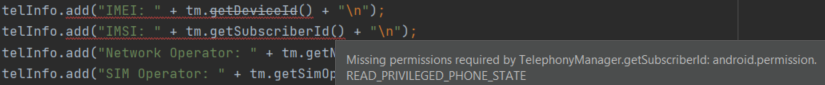
\includegraphics[width=\linewidth]{readpriv}
	\caption{The IDE error upon IMEI and IMSI retrieval actions.}
	\label{imerror}
\end{figure} 
However, the privileged phone state permission is a system permission, and it is impossible to declare and request that permission. Interestingly, these errors also do not block the app from running, and after accepting the requested permission, IMEI and IMSI show up in the permission log along with the other information as follows:
\begin{lstlisting}
--- TELEPHONY --- 
[Phone Type: GSM
, IMEI: 358627081924019
, IMSI: 286039521026739
, Network Operator: Pttcell
, SIM Operator: Pttcell - 28603
, Phone number: +905061901740]

--- BUILD --- 
[Manufacturer: bq, Model: Aquaris X Pro, Serial number: GF006209, Bootloader: BOOT.BF.3.3, Display: 2.11.0_20191121-1510]

--- CALL LOG --- 
[Phone Number: 5331928099 Call Type: 2 Date: Mon Aug 09 18:08:50 GMT+03:00 2021 Duration: 0, 
Phone Number: 5331928099 Call Type: 2 Date: Mon Aug 09 18:09:13 GMT+03:00 2021 Duration: 0, 
Phone Number: 05079776076 Call Type: 1 Date: Mon Aug 09 18:19:20 GMT+03:00 2021 Duration: 49]
\end{lstlisting}
After some research, I found out that the new privileged phone state permişsion was introduced with Android 10, and since this is version is 8.1.0, the error did not make the app crash, just as it did not for the HTC app as well. This of course, means that any app with a minimum SDK less then 29 will have access to this data using the phone state permission.

\subsubsection{Microphone, camera, and sensor permission groups}
The \texttt{android.permission-group.MICROPHONE} is used for permissions that are associated with accessing the microphone. It is noted that phone calls also capture audio, but that functionality is in a separate and more visible permission group. Only one permission is located here, which is \texttt{RECORD\_AUDIO}.

The \texttt{android.permission-group.CAMERA} is used for permissions that are associated with accessing camera or capturing images and video from the device. The only permission here is \texttt{CAMERA}.

The \texttt{android.permission-group.SENSORS} is used for permissions that are related to sensors of the device that capture and measure information about user's body such as heart rate, daily steps (through \texttt{BODY\_SENSORS}) or fingerprint (through \texttt{USE\_FINGERPRINT}).

The permissions in these groups are mostly related to utilizing phone's hardware functionality, thus, they were not demonstrated here.

\subsubsection{Normal permissions}
It was discovered that some information that normal permissions gave access to does not function anymore. Particularly, I found out that many network-related permissions were listed as normal, however, the information gathered was locked behind the location permissions. Therefore, this section contains the analysis of the results gathered from the AppBQ\_none app's code pasted into the full permission state version. The reader may benefit from reading the AppBQ\_none section before this one since the comparisons are drawn based on that.

For the \texttt{wifiInfo()} method, the results are somewhat different. The device Wi-Fi MAC address is blocked from developers completely, so only a meaningless constant value is seen, just as the other version. Connected Wi-Fi SSID and BSSID can clearly be examined this time, whereas the former would return blank, and the latter would return the same constant 02:00:00:00:00:00 in the app with no runtime permissions. The rest of the values have similar results.
\begin{lstlisting}
Device Wi-Fi Mac address: 02:00:00:00:00:00 - Connected Wi-Fi: SSID: Ulas, BSSID: 00:1c:7b:f9:c5:b4, MAC: 02:00:00:00:00:00, Supplicant state: COMPLETED, RSSI: -46, Link speed: 72Mbps, Frequency: 2437MHz, Net ID: 2, Metered hint: false, score: 60
\end{lstlisting}
For comparison, the reader can also see "WIFI-INFO" entry for the AppBQ\_none application.

Previously connected Wi-Fi networks returned the same results, with SSID's and security configurations filled but without MAC addresses. It turns out that this information is not saved, or it is not available after disconnecting.

The Wi-Fi scan was entirely different because without runtime permissions, the scan was not conducted at all. In this version, the scan is conducted, and the scanned networks are written into the log file as such:
\begin{lstlisting}
[SSID: NetMASTER Uydunet-9D7D, BSSID: 3a:6b:1c:03:e9:41, capabilities: [WPA-PSK-CCMP][WPA2-PSK-CCMP][ESS], level: -43, frequency: 2422, timestamp: 1114235528308, distance: ?(cm), distanceSd: ?(cm), passpoint: no, ChannelBandwidth: 1, centerFreq0: 2432, centerFreq1: 0, 80211mcResponder: is not supported, Carrier AP: no, Carrier AP EAP Type: -1, Carrier name: null, 

SSID: Ulas, BSSID: 00:1c:7b:f9:c5:b4, capabilities: [WPA2-PSK-CCMP][ESS], level: -48, frequency: 2437, timestamp: 1114235528390, distance: ?(cm), distanceSd: ?(cm), passpoint: no, ChannelBandwidth: 0, centerFreq0: 0, centerFreq1: 0, 80211mcResponder: is not supported, Carrier AP: no, Carrier AP EAP Type: -1, Carrier name: null, 

SSID: SUPERONLINE_WiFi_7889, BSSID: 94:0b:19:5e:97:0f, capabilities: [WPA-PSK-TKIP+CCMP][WPA2-PSK-TKIP+CCMP][ESS][WPS], level: -80, frequency: 2462, timestamp: 1114235528478, distance: ?(cm), distanceSd: ?(cm), passpoint: no, ChannelBandwidth: 0, centerFreq0: 0, centerFreq1: 0, 80211mcResponder: is not supported, Carrier AP: no, Carrier AP EAP Type: -1, Carrier name: null, 

SSID: TURKSAT-KABLONET-0133-2.4G, BSSID: 18:48:59:1b:49:35, capabilities: [WPA2-PSK-CCMP][ESS], level: -85, frequency: 2472, timestamp: 1114235528561, distance: ?(cm), distanceSd: ?(cm), passpoint: no, ChannelBandwidth: 0, centerFreq0: 0, centerFreq1: 0, 80211mcResponder: is not supported, Carrier AP: no, Carrier AP EAP Type: -1, Carrier name: null]
\end{lstlisting}

For Bluetooth findings, the MAC address and the previously paired devices list returned the same contents with the app's no runtime permissions state. This time, the Bluetooth discovery was not blank and returned the Bluetooth devices that are ready to pair in the environment.
\begin{lstlisting}
[--- Name: OPPO A9 2020 Address: A4:C9:39:AA:4E:2C Contents: 0 Class: 5a020c Type: 1 UUIDs: null---, 
--- Name: Jaybird Tarah Address: C0:28:8D:A1:92:49 Contents: 0 Class: 240404 Type: 1 UUIDs: null---, 
--- Name: [TV] UE65JU7500 Address: FC:8F:90:29:41:3F Contents: 0 Class: 8043c Type: 3 UUIDs: null---]
\end{lstlisting}

\subsection{Permission grants per group}
It is observed that in Android 8.1.0, when a permission is requested, the user is only asked to confirm the group that permission belongs to, as shown in Figure \ref{oninstall}. However, since 6.0, some changes have been made, and requesting one permission from a group does not grant all permissions in that group anymore. Google added the requirement that developer calls \texttt{requestPermissions()} for specific permissions, and not just one of the group. User still grants by the group, but if the developer fails to request the specific permission, the access is not given to that resource.

\section{AppBQ\_none}
For this state of application for the BQ device with Android 8.1.0, the wording for the objective is somewhat changed. This means that no permission state indicates that there are no runtime permissions requested, but the install-time permissions that can be seen in Table \ref{appbqfperms} remain declared. 

The following reasoning is given why the install-time permissions are declared. When the app installation is executed from the .apk file, Android again notifies the user that the app requires no special access. In the AppBQ\_full app, the user could see the install-time permissions along with the runtime permissions in Settings, however, this time user cannot see any declared permissions, even though there are a grand total of 42 permissions declared. This can be seen in Figure \ref{bqnoneappins}. 
\begin{figure}\centering
	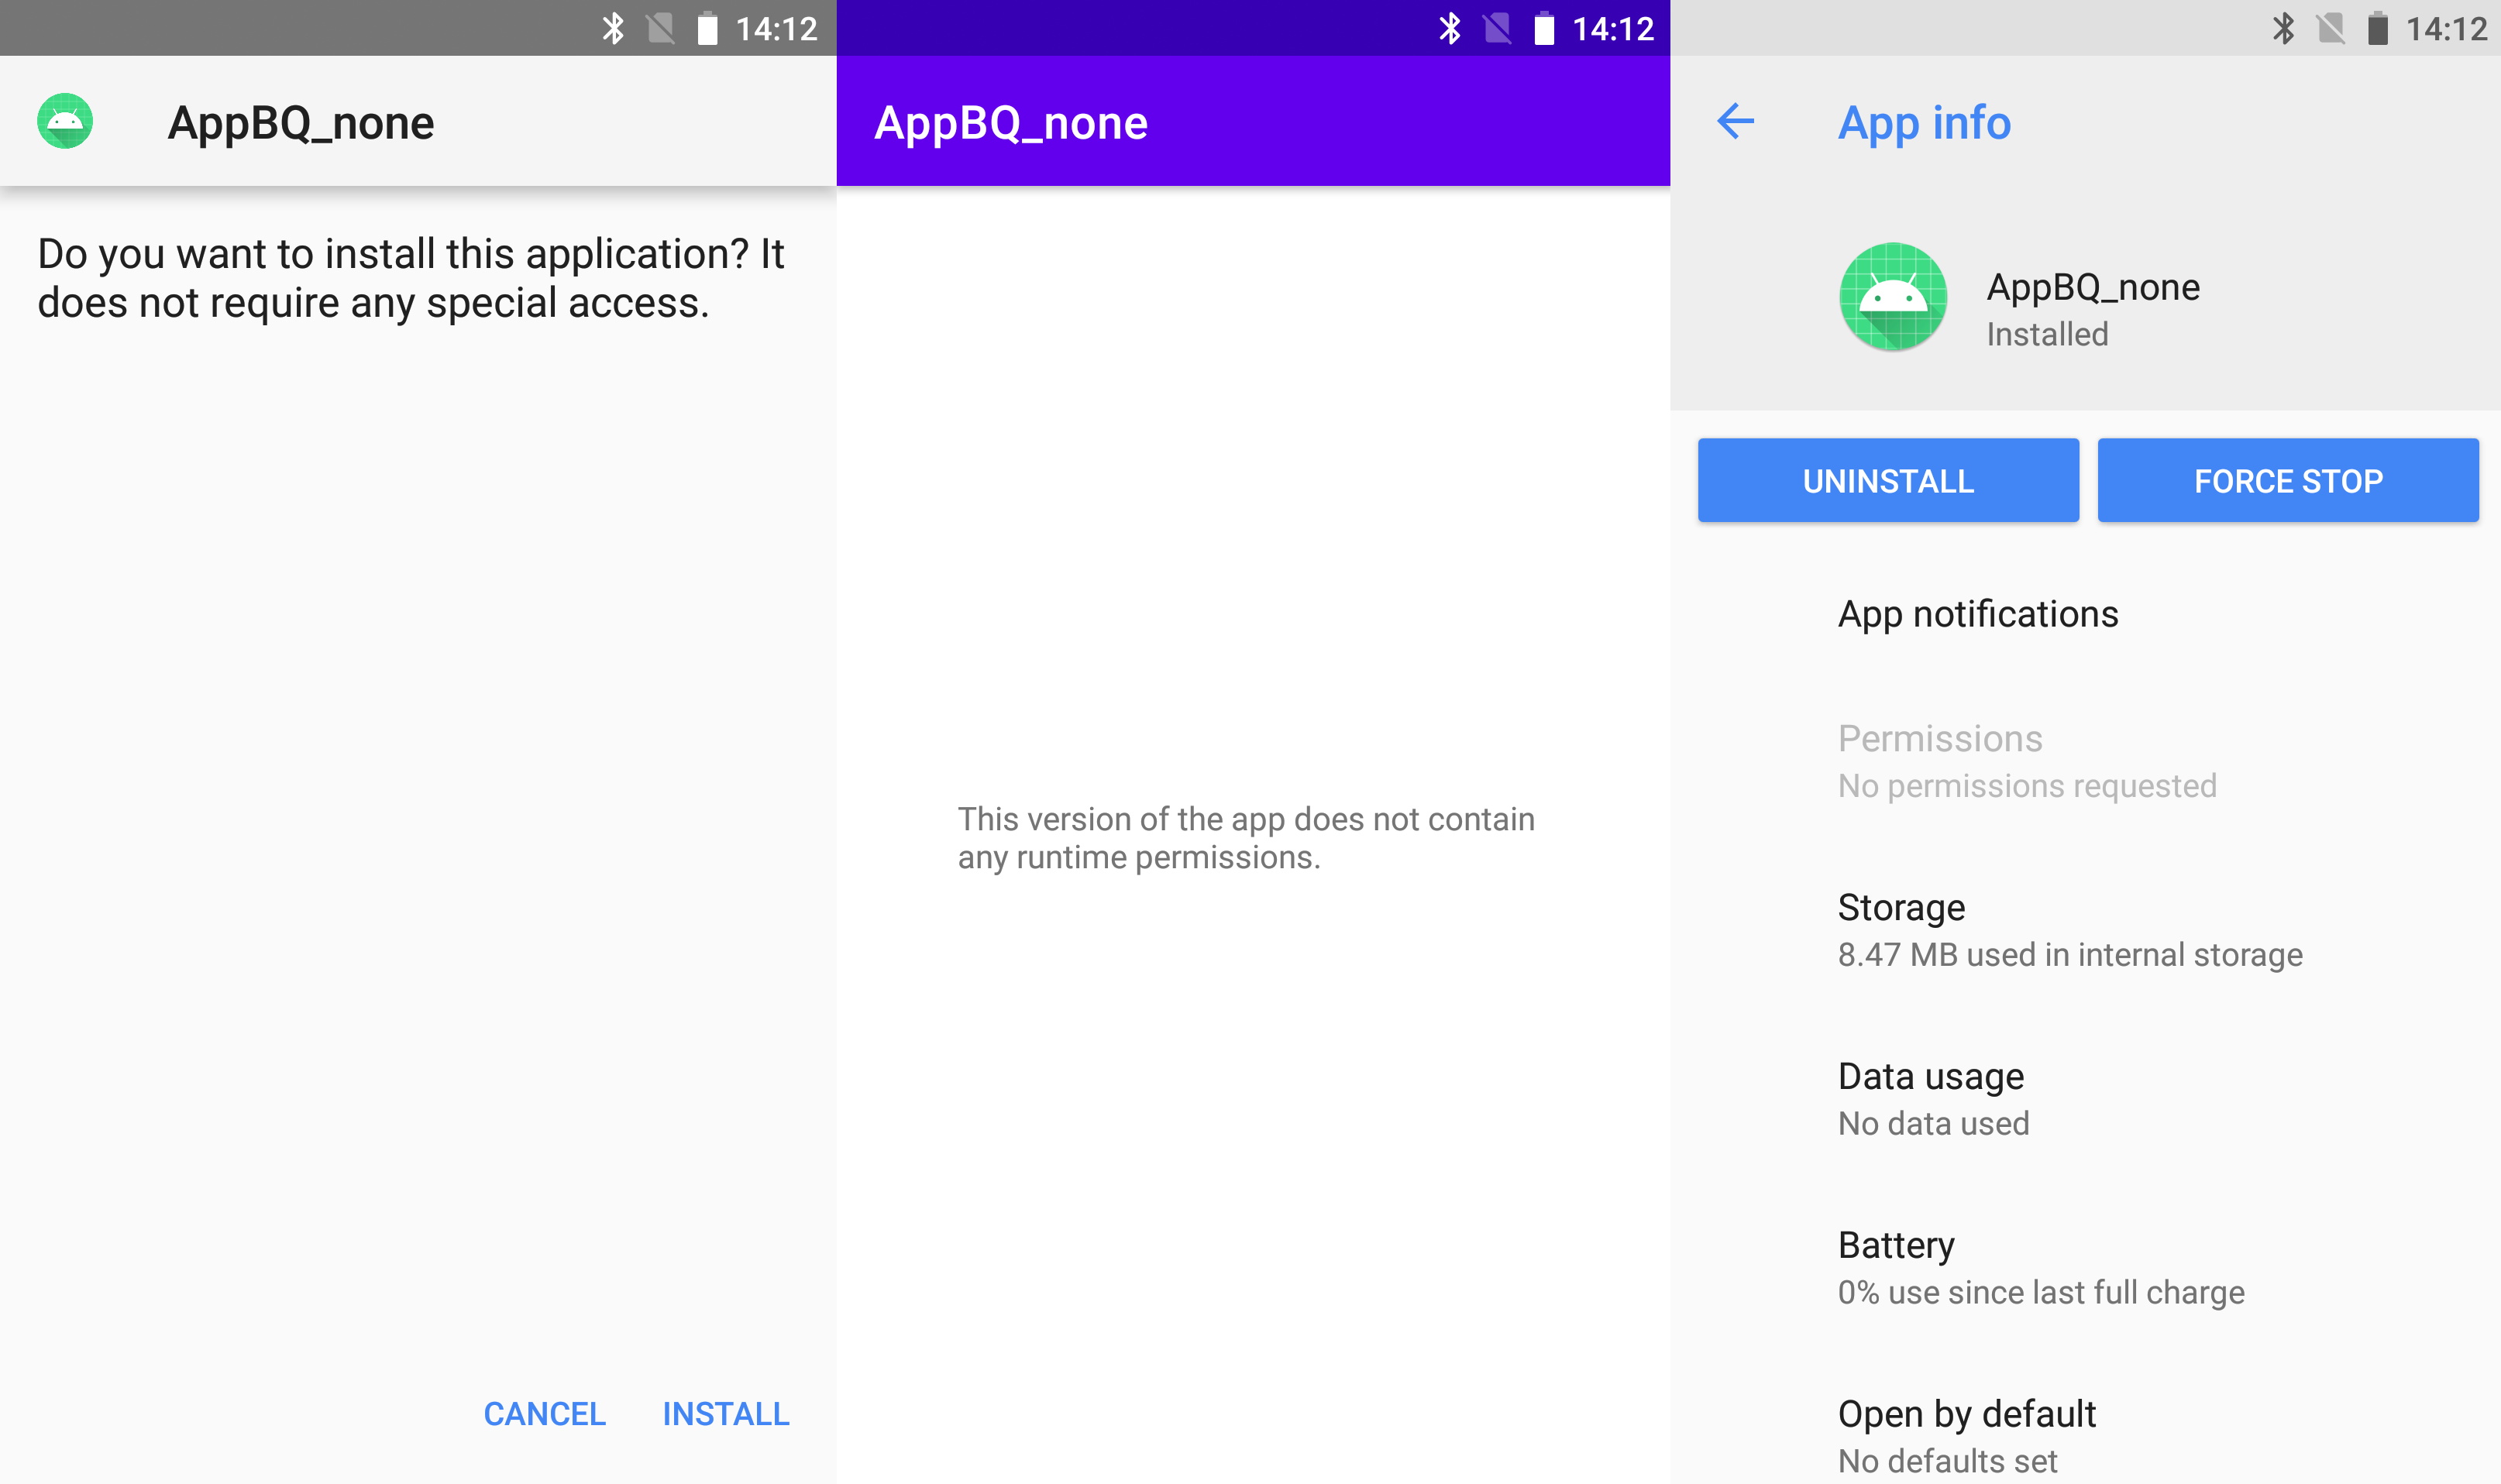
\includegraphics[width=12cm]{bqnoneappins}
	\caption{BQ application installation screens with no permissions requested.}
	\label{bqnoneappins}
\end{figure}
The validity of this was also tested in Android R version 11 (API level 30), which still does not show any declared permissions in Settings for the app. Although it is worth noting that this observation was made on a device created on AVD (Android Virtual Device) Manager, and not with an actual smartphone.

This time the data gathered from the user cannot simply be written into the device storage, since writing and reading external storage permissions are labeled as dangerous and are runtime permissions. There exists some ways to save data on the device across multiple sessions such as Shared preferences API or one of the multiple database APIs that save the data in a local database cache.

\subsection{Shared preferences}
Shared preferences enable the storage of small amounts of primitive data as key/value pairs in a file on the device. To get a handle on a preference file, and to read, write, and manage preference data, the use of \texttt{SharedPreferences} class is appropriate. The Android framework manages the shared preferences file itself. The file is accessible to all the components of the app, but it is not accessible to other apps. Interface for accessing and modifying preference data returned by \texttt{Context.getSharedPreferences(String, int)}. For any particular set of preferences, there is a single instance of this class that all clients share. Modifications to the preferences must go through an Editor object to ensure the preference values remain in a consistent state and control when they are committed to storage. Objects that are returned from the various get methods must be treated as immutable by the application. 

In order to use shared preferences, first  a reference to the shared preference object is created under \texttt{MainActivity} as such:
\begin{lstlisting}
	private SharedPreferences mPreferences;
\end{lstlisting}
Then, in the \texttt{onCreate()} method, shared preferences is initialized using this code:
\begin{lstlisting}
	mPreferences = this.getSharedPreferences(this.getFilesDir().getName(), MODE_PRIVATE);
\end{lstlisting}
The argument \texttt{this.getFilesDir().getName()} returns the folder name of the application's installation path. The other argument \texttt{MODE\_PRIVATE} prevents the shared preferences file to be read by other apps. As a result, an xml file is created inside the app folder, where information can be stored across different sessions (meaning that the app can be closed and opened again, and the information would persist).  

\subsection{Wi-Fi related findings}
As an example of how shared preferences save data, the \texttt{ACCESS\_WIFI\_STATE} permission is used. First, the Wi-Fi state is discovered through the following method:
\begin{lstlisting}
private boolean checkWifiConnection() {
	WifiManager wifiMgr = (WifiManager) getSystemService(WIFI_SERVICE);
	
	if (wifiMgr.isWifiEnabled()) { 
		return true;
	} else {
		return false;
	}
}
\end{lstlisting}
The boolean \texttt{checkWifiConnection()} is a straightforward method that returns a true or false value depending on device Wi-Fi connection. First, an instance of WifiManager is created. Then, \texttt{getConnectionInfo()} method is called from the Wi-Fi manager class, which returns a representational value showing whether the Wi-Fi adapter is on or off. \texttt{getNetworkId()} method from Wi-Fi info class is called as well, in order to see if the active adapter is connected to an access point. If the adapter is on and connected to an AP, the return value is true, else, it is false. 

Since the same classes are being used, a highly simple string method is also created to display all the information stored under \texttt{getConnectionInfo()} method.
\begin{lstlisting}
private String wifiInfo() {
	WifiManager wifiManager = (WifiManager)
		this.getApplicationContext().getSystemService(Context.WIFI_SERVICE);
	String wifiMac = "Device Wi-Fi Mac address: " + wifiManager.getConnectionInfo().getMacAddress();
	String connectedAp = " - Connected Wi-Fi: " + wifiManager.getConnectionInfo().toString();
	return wifiMac + connectedAp;
}
\end{lstlisting}

Together, the information gathered from two methods is written in the \texttt{onPause()} method with shared preferences as seen below.
\begin{lstlisting}
protected void onPause() {
	super.onPause();
	
	SharedPreferences.Editor preferencesEditor = mPreferences.edit();
	if (getApplicationContext().checkCallingOrSelfPermission
			(Manifest.permission.ACCESS_WIFI_STATE)
			== PackageManager.PERMISSION_GRANTED) {
		boolean checkWifi = checkWifiConnection();
		preferencesEditor.putString("CONNECTIVITY", "Connection:" + checkWifi);
		preferencesEditor.putString("WIFI-INFO", wifiInfo());
		preferencesEditor.apply();
	}
}
\end{lstlisting}

As a result, the data is stored under "/data/data/com.example.appbq\_none/shared\_prefs/files.xml", and without any runtime permissions. The "files.xml" file includes the following information inside:
\begin{lstlisting}
<?xml version='1.0' encoding='utf-8' standalone='yes' ?>
<map>
<string name="CONNECTIVITY">Connection:true</string>
<string name="WIFI-INFO">Device Wi-Fi Mac address: 02:00:00:00:00:00 - Connected Wi-Fi: SSID: , BSSID: 02:00:00:00:00:00, MAC: 02:00:00:00:00:00, Supplicant state: COMPLETED, RSSI: -46, Link speed: 72Mbps, Frequency: 2437MHz, Net ID: 2, Metered hint: false, score: 60</string>

</map>
\end{lstlisting}

It is observed that information such as MAC address and SSID is not visible at all, either returning blank or a static meaningless address. This is due to a change that came with Android 6.0; programmatic access to the device's local hardware identifiers using Wi-Fi and Bluetooth APIs is removed \cite{changes60}. Documentation indicates that this change was brought to provide the users increased data protection, so access to things such as SSID are locked behind location runtime permissions, namely \texttt{ACEESS\_FINE\_LOCATION}, or \texttt{ACCESS\_COARSE\_LOCATION}; and access to local hardware identifiers was completely removed. 

Continuing on the Wi-Fi theme, I noticed an interesting issue with the Android Studio. If one tries to get a previously saved network with \texttt{getConfiguredNetworks()}, the IDE will flag it as an error, stating that "Missing permissions required by Wifimanager.getConfiguredNetworks", and names the missing permission as the location access. The method where the error is seen can be viewed below:
\begin{lstlisting}
private String prevConnNetworks() {
	WifiManager wifiManager = (WifiManager)
	this.getApplicationContext().getSystemService(Context.WIFI_SERVICE);
	List<WifiConfiguration> configuredList = wifiManager.getConfiguredNetworks();
	return configuredList.toString();
}
\end{lstlisting}
Normally, an error marked with a red exclamation mark would stop the \textit{Run selected configuration} action. However, when I ignored this error and ran the program, it indeed continued to launch the application without any problems. Writing the return value of this method with to the shared preferences file also did not result in any in-app crashes. To confirm that this is not a general error with my configuration, I conducted some tests. First, I tried different methods that required runtime permissions, such as reading contacts list or getting user accounts. The read contacts method did not contain any errors, but it would crash the app on pause, just as the contacts list was being written into the file. The get accounts method also did not contain any errors, but the entry on the shared preferences file would be blank, exactly the same result when I tried to get connected SSID from the user. With \texttt{prevConnNetworks()}, I wrote the contents of \texttt{getConfiguredNetworks} into the shared preferences file, which includes all saved Wi-Fi SSIDs, key management information, Wi-Fi protocols, pairwise ciphers, and group ciphers pertaining to previously connected networks. Unfortunately, this did not indicate which of the listed networks the device was actually connected to at the moment. Figure \ref{confnet} demonstrates the configured networks entry in the shared preferences file.

\begin{figure}\centering
	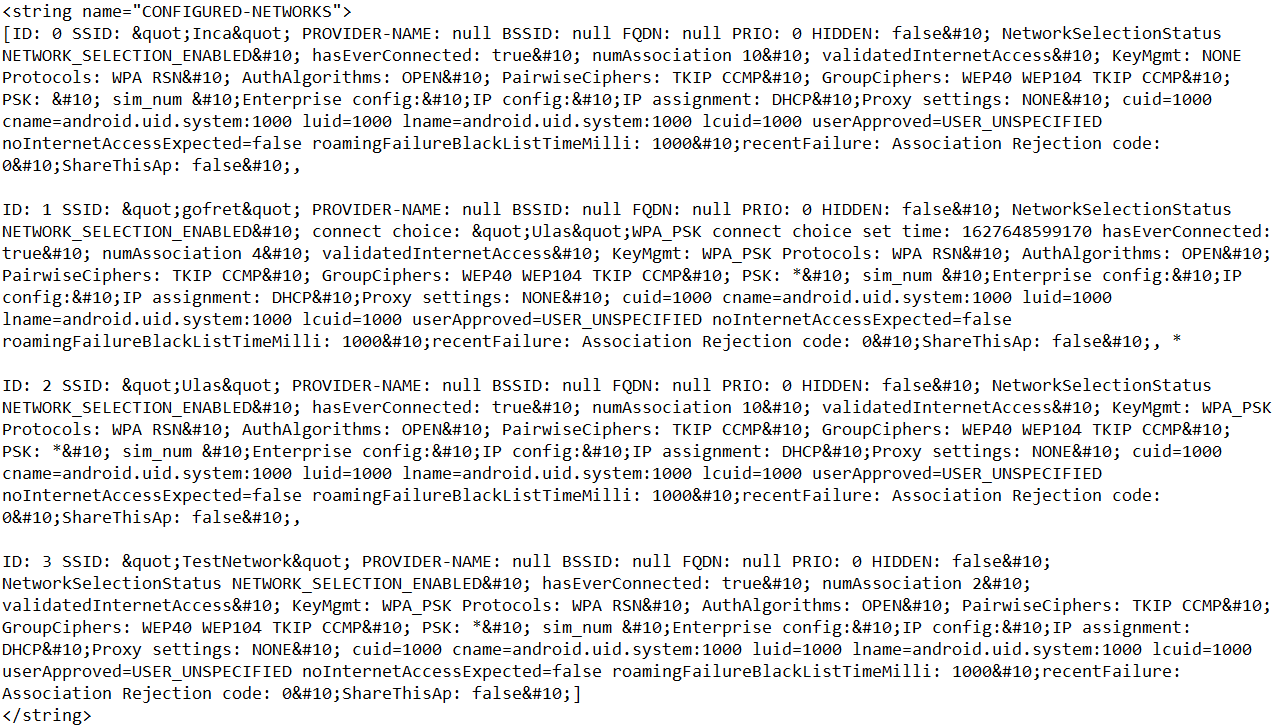
\includegraphics[width=\linewidth]{confnet}
	\caption{The configured networks entry in the shared preferences file.}
	\label{confnet}
\end{figure}

In terms of Wi-Fi connections, there was one remaining thing to check, which was to get a list of available Wi-Fi connections. This is done with \texttt{getScanResults()}, however, it turns out that the method returns no values unless one of the location permissions are enabled. This method can be found in the program code section. It only works when a runtime location permission is requested.

\subsection{Bluetooth related findings}
In order to get information on Bluetooth connections, several approaches can be thought out. These approaches will follow a similar pattern to the Wi-Fi information extraction attempts. I tried to get Wi-Fi information based on the details of the active connection if there were any, previously connected networks, and networks that were available for connection based on an instantaneous scan. In turn, the approaches for Bluetooth would be as follows. First, attempt to find any active connections, following that, try to find the details of previously paired Bluetooth devices, and finally, conduct a scan for any available Bluetooth devices in the area.

A \texttt{getConnBtDevice()} method was created to get details of the connected Bluetooth device. Within this method, an instance of the Bluetooth manager was created, which enabled me to use the available \texttt{getConnectedDevices()} method, which is supposed to return the set of devices that is in the \textit{connected} state as such:
\begin{lstlisting}
List<BluetoothDevice> btDevice = bluetoothManager.getConnectedDevices(GATT_SERVER);
\end{lstlisting}
The \texttt{btDevice} was used as the return value of the method. This did not result in any visible errors, however, it caused the app to crash. This happened even when the location permission was requested temporarily to test this, and the result was the same. Therefore, extracting the connected device name was a failure. 

The next goal was to get information on the paired Bluetooth devices. The \texttt{btDiscoverDevices()} method was created to achieve this. The method can be seen down below:
\begin{lstlisting}
private String btDiscoverDevices() {
	BluetoothAdapter bluetoothAdapter = ((BluetoothManager)
	this.getApplicationContext().getSystemService(Context.BLUETOOTH_SERVICE)).getAdapter();

	bluetoothAdapter.startDiscovery();

	IntentFilter filter = new IntentFilter(BluetoothDevice.ACTION_FOUND);
	registerReceiver(btBroadcastReceiver, filter);

	return btDeviceList.toString();
}
\end{lstlisting} 
The method first creates an instance of the Bluetooth adapter, then starts the remote device discovery process. The result is sent to the broadcast receiver, which is a base class for code that handles broadcast intents. There, the list string \texttt{btDeviceList} is filled with information pertaining to the found devices, and used as the return value of the \texttt{btDiscoverDevices()} method. Finally, the contents of the return value are saved to the shared preferences file. Unfortunately, this returned a blank string. It was observed that when one of the location permissions were requested, the list would be filled up by available Bluetooth devices, thus, this action also was locked behind the location permissions. Similar to Wi-Fi findings, these first two operations were a failure.

Finally, I tried to get a list of previously paired Bluetooth devices. It was done through a simple method called \texttt{getPairedBt()}, which can be observed below:
\begin{lstlisting}
private String getPairedBt() {
	BluetoothAdapter bluetoothAdapter = ((BluetoothManager)
	this.getApplicationContext().getSystemService(Context.BLUETOOTH_SERVICE)).getAdapter();
	
	Set<BluetoothDevice> btDeviceList = bluetoothAdapter.getBondedDevices();
	
	List<String> list = new ArrayList<>();
	for(BluetoothDevice bluetoothDevice : btDeviceList) {
		list.add("--- Name: " + bluetoothDevice.getName());
		list.add("Address: " + bluetoothDevice.getAddress());
		list.add("Contents: " + bluetoothDevice.describeContents());
		list.add("Class: " + bluetoothDevice.getBluetoothClass());
		list.add("Type: " + bluetoothDevice.getType());
		list.add("UUIDs: " + bluetoothDevice.getUuids() + "---");
	}
	return list.toString();
}
\end{lstlisting}
The method simply creates an instance of the Bluetooth adapter, then assigns the return value of Bluetooth adapter member method \texttt{getBondedDevices()} to a Bluetooth device set variable. This information is written into a list with a loop and finally, the list is used as the string return value. This value is then written into the shared preferences file. The entry in the file looks as such:
\begin{lstlisting}
    <string name="PAIRED-BT">
    [--- Name: Cagri (main), Address: 20:EE:28:E3:44:0D, Contents: 0, Class: 7a020c, Type: 2, UUIDs: [Landroid.os.ParcelUuid;@38a581b---, 
    --- Name: Jaybird Tarah, Address: C0:28:8D:A1:92:49, Contents: 0, Class: 240404, Type: 1, UUIDs: [Landroid.os.ParcelUuid;@8a1edb8---]</string>
\end{lstlisting}
The two devices were paired as an example to the BQ device, one of which is an iPhone 7, and the other is a Bluetooth Jaybird Tarah earphone. Interestingly, this method neither created any errors in the IDE nor during runtime. Names of the previously paired devices, and their Bluetooth MAC addresses are clearly visible. 

Consequently, the Bluetooth findings coincided with the Wi-Fi findings, where only the previously configured and/or paired devices were extracted without any (runtime) permissions.

\subsection{NFC related findings}
Even though the \texttt{NFC} permission was declared, I was in possession of no NFC tags, and could not put it to test.

\subsection{Unique identifiers}
Without using any permissions, one can also get a unique identifier using Secure Android ID. While this identifier is a constant, it is not hard-coded to the device. A factory reset or an OS upgrade can reset this value, leading the device to have a different identifier. However, it is observed that this value stays the same regardless of app restart, reinstall, or device restart. The following function is used to get this ID, using the Settings provider.
\begin{lstlisting}
private String getSecureId() {
	String androidId = Settings.Secure.getString(getContentResolver(), Settings.Secure.ANDROID_ID);
	return androidId;
}
\end{lstlisting}
Return value \texttt{androidId} is written to the shared preferences file as such:
\begin{lstlisting}
<string name="SECURE-ANDROID-ID">9aad5b2905182c59</string>
\end{lstlisting}

\section{AppHTC\_full}
This is the full permission state application for the HTC One SV device which carries Jelly Bean 4.2.2 (API level 17) version of Android. Documentation indicates that permissions also were categorized, although somewhat differently from the API level 27. In addition, these permission groups aren't depicted to the user in the UI side of the coin and may be done so out of a concern for developer convenience, for both Android application developers and for the ones who contribute to the Android platform itself. 

When the user taps on the .apk file for installation, the device simply states "Do you want to install this application? It will get access to:", and lists every declared permission regardless of protection level or permission group. This can be seen in Figure \ref{htcappinstall}.
\begin{figure}\centering
	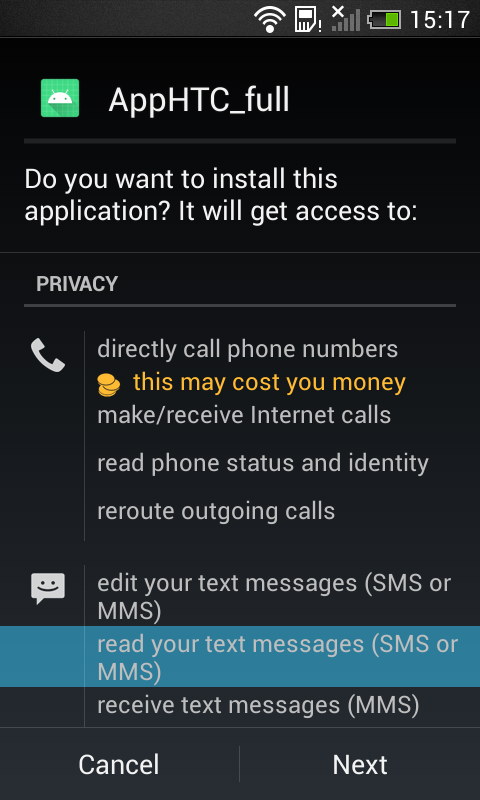
\includegraphics[width=6cm]{htcappinstall}
	\caption{HTC device permission prompt on app install.}
	\label{htcappinstall}
\end{figure}

The full permission list for this app can be seen in Table \ref{apphtcfperms}. In this section, the permissions related to the scope of this thesis will be examined by groups. These are the permissions that let us read or receive information related to the user.

First on the list is the MESSAGES group. Within it, \texttt{RECEIVE\_SMS} and \texttt{READ\_SMS} permissions are of some interest. The MMS and WAP push permissions are ignored since almost everyone uses instant messaging applications instead. The SMSs in the device are located in the internal Android SMS table. As such, the information will be gathered from the table by rows and tables. Here is what the function \texttt{readSms()} looks like this:
\begin{lstlisting}
private String readSms() {
	Cursor c = getContentResolver().query(Uri.parse("content://sms/inbox"),
	null, null, null, null);
	String message = "";
	if (c.moveToFirst()) {
		do {
			for (int i = 0; i < c.getColumnCount(); i++) {
				if (c.getColumnName(i).equals("date")) {
					Date date = new Date(c.getLong(i));
					message += " Date: " + date +" / ";
				}
				else if (c.getColumnName(i).equals("address")) {
					message += " Address: " + c.getString(i) + " / ";
				}
				else if (c.getColumnName(i).equals("body")) {
					message += " Message body: " + c.getString(i) + "\n";
				}
			}
		} while (c.moveToNext());
	} else {
		return "No messages to log!";
	}
	c.close();
	return message;
}
\end{lstlisting}
The SMS table includes two columns for the entry name and value, and various rows for the types of data the SMS message holds. For demonstration, I select the column names that are equal to "date", "address", and "body", and add them to the string variable message, which will be the return value of the function. If the table is empty, the return value indicates that there are no messages to log, if there are any, it is written into the permission log file, and the portion that is written to the text file is as following:
\begin{lstlisting}
	 Address: +905459430635 /  Date: Wed Jul 28 16:32:55 EEST 2021 /  Message body: Another test message
	Address: +905459430635 /  Date: Wed Jul 28 16:32:40 EEST 2021 /  Message body: Test message
\end{lstlisting}
Two messages were sent from another device consecutively, and it can be seen that they are written into the file with the sender number, date sent, and what the message contains. 

A broadcast receiver was used to pick up the incoming SMS message that is given access by the \texttt{RECEIVE\_SMS} permission. The receiver is registered with the onCreate() method, and listens for the SMS received action. In the method, the incoming message body and sender number is extracted, and the date is noted at the time of arrival. Then, the contents are written into the permission logs file, and the broadcast receiver is unregistered with the onDestroy() method. The contents of the receiver can be seen below:
\begin{lstlisting}
private static final String SMS_RECEIVED = "android.provider.Telephony.SMS_RECEIVED";
List<String> receivedMessage = new ArrayList<>();
private final BroadcastReceiver smsBr = new BroadcastReceiver() {
	@Override
	public void onReceive(Context context, Intent intent) {
		Bundle bundle = intent.getExtras();
		SmsMessage[] messages;
		String messageAddr = "";
		String body = "";
		if (bundle != null) {
			try {
				Object[] pdus = (Object[]) bundle.get("pdus");
				messages = new SmsMessage[pdus.length];
				for (int i = 0; i < messages.length; i++) {
					messages[i] = SmsMessage.createFromPdu((byte[])pdus[i]);
					messageAddr += messages[i].getDisplayOriginatingAddress();
					body += messages[i].getMessageBody();
				}
				receivedMessage.add("Message Address: " + messageAddr +
				", Message body: " + body +
				", Time received: " + Calendar.getInstance().getTime());
				logToFile(getApplicationContext(), receivedMessage.toString());
			} catch (Exception e) {
				Log.d("Exception caught ", e.getMessage());
			}
		}
		else {
			logToFile(getApplicationContext(), "\nBundle is null.");
		}
	}
};0
\end{lstlisting}

To test if it works, a SIM was inserted into the device and a message was sent to the same phone number. The resulting SMS was picked up and written to the file by the receiver. The resulting file entry can be seen below:
\begin{lstlisting}
[Message Address: +905331928099, Message body: Message to myself: test receive sms , Time received: Tue Aug 03 19:01:26 EEST 2021]
\end{lstlisting}

SOCIAL\_INFO group includes the permissions that provide access to the user's social data, such as contacts, the call log, and the social stream. Normally, three permissions would be tested in this group, namely, \texttt{READ\_CONTACTS}, \texttt{READ\_CALL\_LOG}, and \texttt{READ\_SOCIAL\_STREAM}. However, the latter permission which deals with the social stream is not really functional anymore. It would give access to the social media application's stream of data related to friends, family, and followed people. However, since then, these social media apps have changed how they work on their end, and do not necessarily share this data with the device OS. Thus, I argue that this relic of a permission does not need further effort.

So for the reading contacts permission, a similar action to the SMS method is required. That is to say, the information regarding the contacts is stored under a table, and extraction includes using the cursor to find the desired columns, and storing the related information to a variable as seen below:
\begin{lstlisting}
private String getContacts() {
	List<String> contactList = new ArrayList<String>();
	ContentResolver cr = getContentResolver();
	Cursor c = cr.query(ContactsContract.Contacts.CONTENT_URI, null, null, null, null);
	if ((c != null ? c.getCount() : 0) > 0) {
		while (c.moveToNext()) {
			String id = c.getString(c.getColumnIndex(ContactsContract.Contacts._ID));
			String name = c.getString(c.getColumnIndex(ContactsContract.Contacts.DISPLAY_NAME));
			contactList.add(name);
			if (c.getInt(c.getColumnIndex(ContactsContract.Contacts.HAS_PHONE_NUMBER)) > 0) {
				Cursor pCur = cr.query(ContactsContract.CommonDataKinds.Phone.CONTENT_URI, null,
				ContactsContract.CommonDataKinds.Phone.CONTACT_ID + " = ?", new String[]{id}, null);
				while (pCur.moveToNext()) {
					String phoneNo = pCur.getString(pCur.getColumnIndex(ContactsContract.CommonDataKinds.Phone.NUMBER));
					contactList.add(phoneNo);
				}
				pCur.close();
			}
		}
	}
	if (c != null) {
		c.close();
	}
	return contactList.toString();
}
\end{lstlisting}

I added three different contacts with random telephone numbers, and as a result, the method finds this information and stores it into the permission log file. 
\begin{lstlisting}
[Contact A, 05329990099, Contact B, 05331234567, Contact C, 05340008521]
\end{lstlisting}

As such, the call log is also stored in a local table, and the \texttt{getCallLog()} method's contents are quite similar to the contacts and the SMS methods.
\begin{lstlisting}
private String getCallLog() {
	ContentResolver cr = getContentResolver();
	Cursor c = cr.query(CallLog.Calls.CONTENT_URI, null, null, null, null);
	List<String> callList = new ArrayList<>();
	while (c.moveToNext()) {
		Date date = new Date(c.getLong(c.getColumnIndex(CallLog.Calls.DATE)));
		callList.add("\nPhone Number: " + c.getString(c.getColumnIndex(CallLog.Calls.NUMBER)) +
		" Call Type: " + c.getString(c.getColumnIndex(CallLog.Calls.TYPE)) +
		" Date: " + date +
		" Duration: " + c.getString(c.getColumnIndex(CallLog.Calls.DURATION)));
	}
	
	c.close();
	return callList.toString();
}
\end{lstlisting}

Some calls were made to various random numbers, and since the phone did not include a SIM card within, the calls were immediately halted. The duration is always zero as it can be seen below. Other than that, the permission log entry includes the phone number, type of call (outgoing, incoming etc.), date, and duration.
\begin{lstlisting}
	[Phone Number: 05329990099 Call Type: 2 Date: Tue Aug 03 17:09:41 EEST 2021 Duration: 0, 
	Phone Number: 05340008521 Call Type: 2 Date: Tue Aug 03 17:09:52 EEST 2021 Duration: 0, 
	Phone Number: 05340008521 Call Type: 2 Date: Tue Aug 03 17:10:00 EEST 2021 Duration: 0, 
	Phone Number: 05331234567 Call Type: 2 Date: Tue Aug 03 17:10:05 EEST 2021 Duration: 0]
\end{lstlisting}

The next group is named PERSONAL\_INFO, and has two permissions, which is related to reading and writing of user profile. Just like before, a content resolver is used to query the related entry, which is \texttt{ContactsContract.Profile} this time, and a cursor is defined to navigate to the display name and id. The method \texttt{getProfile()} is as follows:
\begin{lstlisting}
private String getProfile() {
	ContentResolver cr = getContentResolver();
	Cursor c = cr.query(ContactsContract.Profile.CONTENT_URI, null, null, null, null);
	List<String> profile = new ArrayList<>();
	while (c.moveToNext()) {
		profile.add("Name: " + c.getString(c.getColumnIndex(ContactsContract.Profile.DISPLAY_NAME)) +
		" - ID: " + c.getString(c.getColumnIndex(ContactsContract.Profile._ID)));
	}
	c.close();
	return profile.toString();
}
\end{lstlisting}
The permission log entry includes the user e-mail, and an ID value, which may represent the user account.
\begin{lstlisting}
[Name: Cagri HTC Erdem - ID: 9223372034707292161]
\end{lstlisting}

CALENDAR permission group includes the permissions that allow an application to read and write calendar data. The method \texttt{getCalendar()} was used in AppBQ\_full app, and it will also be used here. One can view the method in Calendar permission group section or the GitHub page with the full codes. It demonstrates how and what kinds of data are being read.

As it can be seen below, calendar details such as future event titles, places, and times they take place are saved in the permission log file.
\begin{lstlisting}
[account name: PC Sync
calendar display name:HTC Sync Manager
title: Important event 1
location: Offenburg, Offenburg, Germany
event start: Mon Aug 09 03:00:00 EEST 2021
event end: Tue Aug 10 03:00:00 EEST 2021, 
account name: PC Sync
calendar display name:HTC Sync Manager
title: Unimportant event 99
location: Süleymanpasa/Tekirdag, Turkey
event start: Wed Aug 11 03:00:00 EEST 2021
event end: Thu Aug 12 03:00:00 EEST 2021]
\end{lstlisting}

Since the code is getting quite repetitive, I skipped the user dictionary group which had the \texttt{READ\_USER\_DICTIONARY} permission. Instead, the full codes found in the Android Studio project folders can be examined in the GitHub link given in Section 4.2 or \cref{cha:discussion}. Following that, it is observed that the bookmarks group has also lost its functionality due to the changes on the browser end. The history bookmarks would normally be reported by the browser to the OS in the old days, however since then, Android stopped this and effectively deprecated the permission, making this change valid for all versions. Another similar example will come up with the telephony group later.

The method for the location permission group works exactly like the one for the BQ full app, so the code and the results are identical. One can refer to the BQ full findings, or the GitHub page to view it.

The methods related to Wi-Fi and Bluetooth permissions stayed practically the same as ones for the BQ device, however, the results have differences. In this version, the device Wi-Fi and Bluetooth MAC addresses aren't locked, and return the actual value instead of a meaningless constant.
\begin{lstlisting}
Device Wi-Fi Mac address: 1c:b0:94:a4:47:39 - Connected Wi-Fi: SSID: Ulas, BSSID: 00:1c:7b:f9:c5:b4, Supplicant state: COMPLETED, RSSI: -70, Link speed: 39, Frequency: 2412, Net ID: 1, Metered hint: false

Bluetooth MAC Address: BC:CF:CC:C1:FC:7A
\end{lstlisting}
Other than that, the information pertaining to the connected AP, discovered Wi-Fi networks and Bluetooth devices, and previously connected networks and paired devices resulted in the same outcome with the AppBQ\_full.

The ACCOUNTS group included the saved accounts, and just as the same before, I could get the user Gmail with the same code in the \texttt{getAcc()} method. The difference is that the user e-mail can also be retrieved from the calendar and profile-related methods in this app.

PHONE CALLS group had one interesting candidate, namely the  \texttt{READ\_PHONE\_STATE} permission. Two methods were created to retrieve the related information. First method is \texttt{getTelephonyInfo()}. The contents are as follows:
\begin{lstlisting}
private String getTelephonyInfo() {
	TelephonyManager tm = (TelephonyManager) getSystemService(Context.TELEPHONY_SERVICE);
	List<String> telInfo = new ArrayList<>();
	
	String phoneType = null;
	if (tm.getPhoneType() == TelephonyManager.PHONE_TYPE_GSM)
	phoneType = "Phone Type: GSM\n";
	else if (tm.getPhoneType() == TelephonyManager.PHONE_TYPE_CDMA)
	phoneType = "Phone Type: CDMA\n";
	telInfo.add(phoneType);
	telInfo.add("IMEI: " + tm.getDeviceId() + "\n");
	telInfo.add("IMSI: " + tm.getSubscriberId() + "\n");
	telInfo.add("Network Operator: " + tm.getNetworkOperatorName() + "\n");
	telInfo.add("SIM Operator: " + tm.getSimOperatorName() + " - " + tm.getSimOperator() + "\n");
	telInfo.add("Phone number: " + tm.getLine1Number());
	return telInfo.toString();
}
\end{lstlisting}
In this method, an instance of the telephony manager object is created to get relevant information. First, the phone type is determined and the result is saved to the string list. Following that, the IMEI, IMSI, Network and SIM operator names, and phone number are written into the list which is returned by the method. The \texttt{telInfo} string list is then written into the permission log file. The results clearly show the retrieved data.
\begin{lstlisting}
[Phone Type: GSM
, IMEI: 355026055113951
, IMSI: 286016296911274
, Network Operator: Turkcell
, SIM Operator: Turkcell - 28601
, Phone number: +905331928099]
\end{lstlisting} 

The second method \texttt{getBuildInfo()} includes information affiliated with the current device build extracted from the system properties.
\begin{lstlisting}
private String getBuildInfo() {
	List<String> buildInfo = new ArrayList<>();
	
	buildInfo.add("Manufacturer: " + Build.MANUFACTURER);
	buildInfo.add("Model: " + Build.MODEL);
	buildInfo.add("Serial number: " + Build.SERIAL);
	buildInfo.add("Bootloader: " + Build.BOOTLOADER);
	buildInfo.add("Display: " + Build.DISPLAY);
	
	return buildInfo.toString();
}
\end{lstlisting} 
This method gets the manufacturer name, device model, device serial number, bootloader version number, and the firmware build ID.
\begin{lstlisting}
[Manufacturer: HTC, Model: HTC One SV, Serial number: SH2CVTP01483, Bootloader: 2.21.0000, Display: JDQ39]
\end{lstlisting}

Lastly, using the phone state permission, I tried to get the relevant cell tower details but this was a failure. In the old versions, the documentation included the method \texttt{getNeighboringCellInfo()} to get this information, however,  it turns out that Android has deprecated this method after 2015, and completely removed it in Android Q. A method called \texttt{getAllCellInfo()} was added, however sub-methods such as \texttt{getCellIdentity()} was only available for applications with the minimum SDK level 30. In addition, Android added a new system-reserved permission called \texttt{READ\_PRIVILEGED\_PHONE\_STATE}, which outright blocks every application from retrieving this information regardless of the version, except the system apps.

%read external storage remaining

\section{AppHTC\_none}
For this version, every permission declared shows up upon installation and in the Settings. Staying in objective scope for this app means that no permissions can be declared in any way. The first order of business, is to try the AppBQ\_none code in this app. After some small adjustments to make it work in the older SDK level app, and some lint suppressions to disregard the errors, it was launched. However, this immediately resulted in a crash.

Next, the lint suppressors were removed, and the erroneous code was commented out to see the remaining information. This in turn, downright eliminated some methods such as \texttt{prevConnNetworks()} (previously connected Wi-Fi networks), \texttt{getBtInfo()} (Bluetooth MAC), \texttt{btDiscoverDevices()}(Bluetooth discovery method), and finally, \texttt{getPairedBt()} (previously bonded Bluetooth devices). The remaining entries in the shared preferences file were Wi-Fi info, Wi-Fi scan, and secure Android ID. Interestingly, this also resulted in a direct crash. It turned out that even the remaining methods without any errors made the app crash, and in the end, the only piece of information gathered from the device was the secure Android ID, which as I mentioned before, is not a completely sound way of retrieving an identifier, since it can be changed to another value after a factory reset, or version update.

\section{Findings on the rooted devices}
The root access was given to the BQ device through Magisk Manager, and to the HTC device through the SuperSU app. Both applications are similar in what they do, which gives superuser access to the user, and enables applications to run \textit{su} commands in their code, provided that the user agrees to give them this access. The root access was done on the stock ROM with the same Android versions, so virtually nothing was changed on the devices except the access to superuser privileges for the device user. 

Rooting the device does not change anything for what the applications return in the log files, since this privilege is given to the user and not the app. The user still needs to grant the superuser request by prompted the app. Following this, I set up two more apps to test these shell commands through Java. The point here is to get information relevant to the scope of this thesis without any permission. 

For the BQ device, a \texttt{runCommand()} method was implemented. The method takes a shell command as argument, and writes it into standard input of a su process.
\begin{lstlisting}
public void runCommand(String...commands) {
	try {
		Process process = Runtime.getRuntime().exec("su");
		DataOutputStream dataOutputStream = new DataOutputStream(process.getOutputStream());
		for(String s : commands) {
			dataOutputStream.writeBytes(s + "\n");
			dataOutputStream.flush();
		}
		dataOutputStream.writeBytes("exit\n");
		dataOutputStream.flush();
		try {
			process.waitFor();
		} catch(Exception e) {
			logToFile(this, e.getMessage());
		}
		logToFile(this, "recording saved.");
		dataOutputStream.close();
	} catch (Exception e) {
		logToFile(this, e.getMessage());
	}
}
\end{lstlisting}
When this method is called with a shell command, the application receives a prompt from Magisk app, givin the option to grant or deny the superuser request as seen in Figure \ref{sureq}.
\begin{figure}\centering
	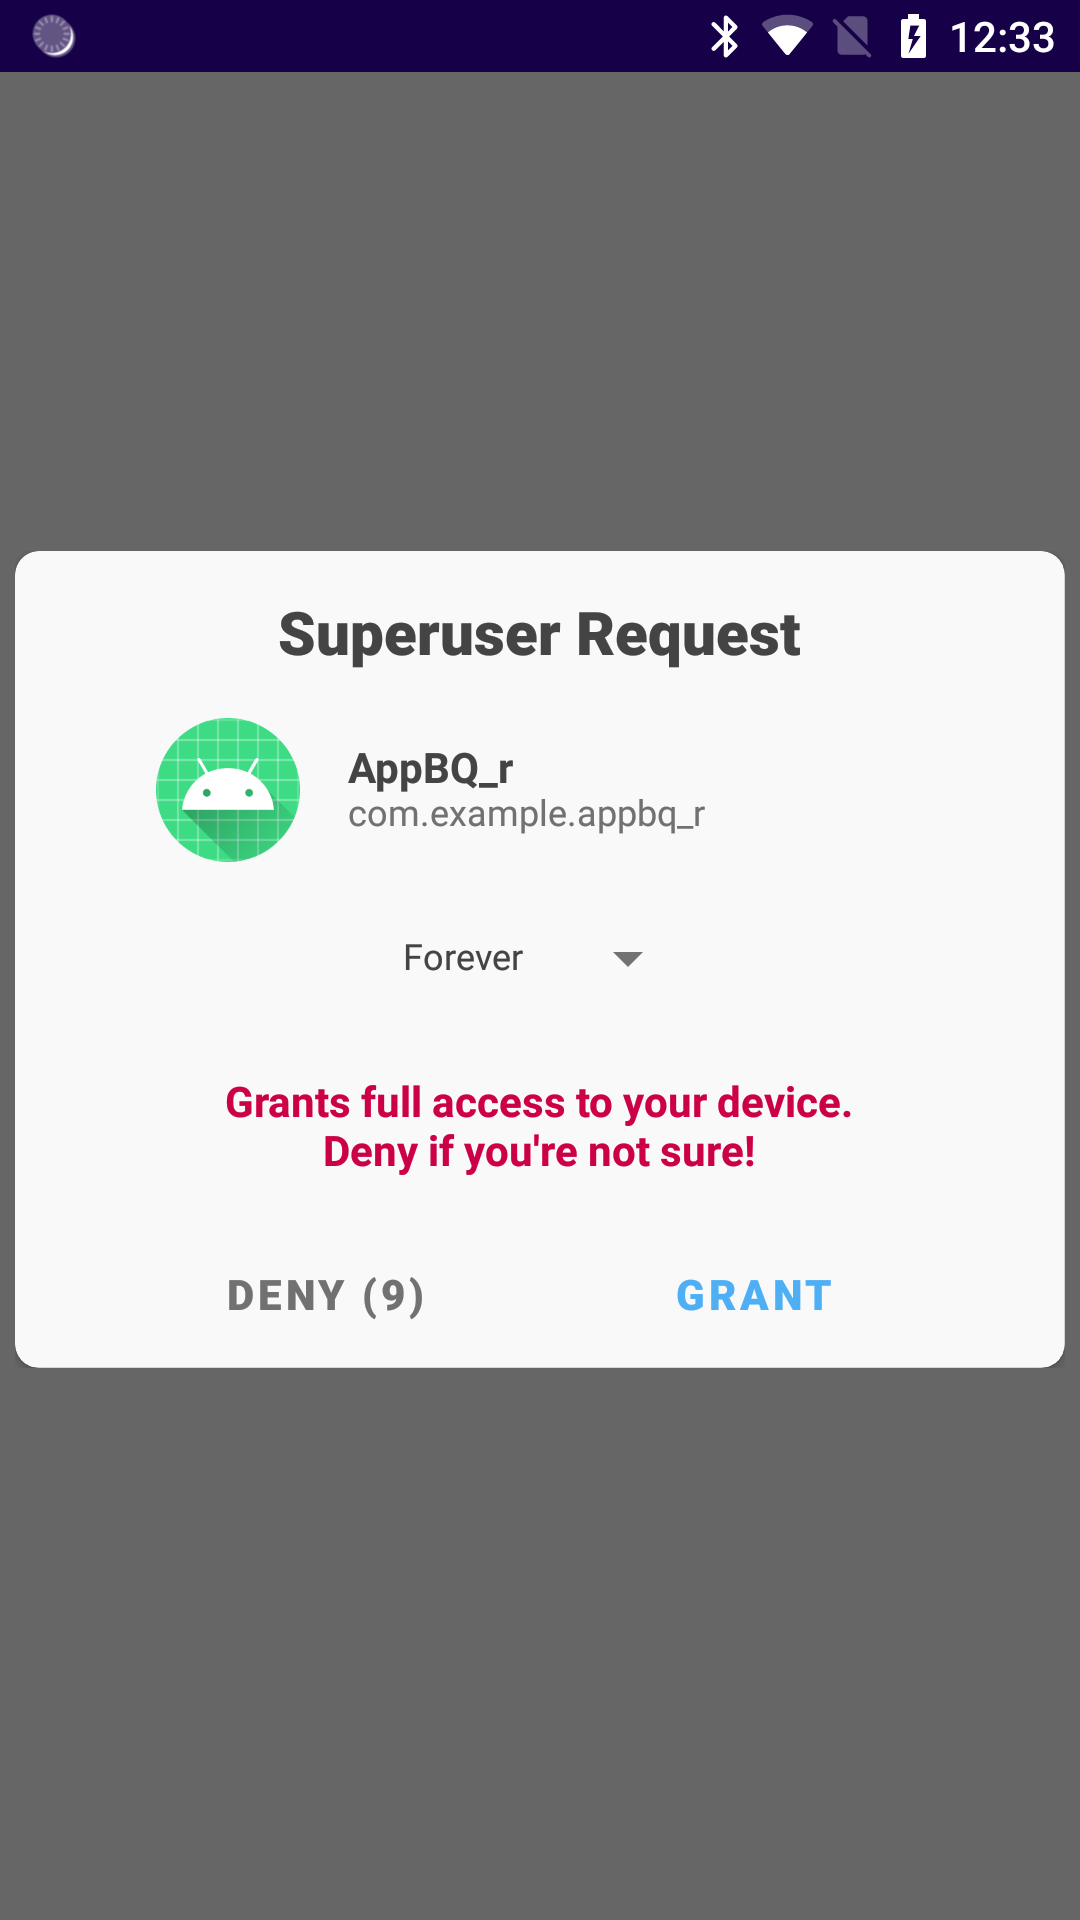
\includegraphics[width=6cm]{sureq}
	\caption{Magisk prompt to regarding superuser access on the BQ device.}
	\label{sureq}
\end{figure}
A Google Developers page that lists the Android Debug Bridge (adb) shell commands is available \cite{adbshellcmd}. After granting the superuser request, the app functions as normal. I wrote some commands from the adb shell command list in order to try the \texttt{runCommands()} method as seen below:
\begin{lstlisting}
runCommand("screenrecord --time-limit 5 "
+ getApplicationContext().getFilesDir() + "/sRec.mp4\n");
runCommand("screencap "
+ getApplicationContext().getFilesDir() + "/screen.png");
\end{lstlisting}
The first command is supposed to record the screen for 5 seconds, and the second to take a screenshot. After these actions are completed, a process completion note to the log file is written for each process. The screen.png and sRec.mp4 is supposedly saved to the files folder in the application directory. Device File Explorer in Android Studio confirms this fact. From the file sizes, one can tell that the recording and screenshotting actions are actually being completed. If I change the time limit for the recorder, the sRec.mp4 file increases in size. However, when I try to save the files, copy them, or simply open them, Device File Explorer gives the following error:
\begin{lstlisting}
Error opening contents of device file "screen.png": cp: /data/local/tmp/temp7eac41bc-4f0a-4d9d-a6e3-686823b7b656: Permission denied
\end{lstlisting}
Interestingly, on Windows File Explorer, these files were invisible, as in they were not set as invisible, they were simply not there. Android's file explorer showed screen.png to be 39.4 KB, and the sRec.mp4 to be 745.4 KB, however when I looked at the same location from the Windows' explorer with the address \texttt{AppData\textbackslash Local\textbackslash Google\textbackslash AndroidStudio2020.3\textbackslash device-explorer
\textbackslash bq-aquaris\_x\_pro-GF006209\textbackslash data\textbackslash data\textbackslash com.example.appbq\_r\textbackslash files}, the total size of the folder was 56 bytes, the exact same value as the plogs.txt file located in the same place. The \texttt{data/local/tmp} folder was also nowhere to be seen in Windows file explorer, and showed up as empty in Android device file explorer. To mitigate this problem, I wrote \texttt{chmod 777} superuser command to change the permissions in the folder.
\begin{lstlisting}
try {
	Runtime.getRuntime().exec("chmod -R 777 " + getApplicationContext().getFilesDir());
	Runtime.getRuntime().exec("chmod -R 777 " + "/data/local/tmp");
} catch (Exception e) {
	logToFile(this, e.getMessage());
}
\end{lstlisting}
This actions results in a change to permissions somewhat, which can be observed in Figure \ref{permnoch}.
\begin{figure}\centering
	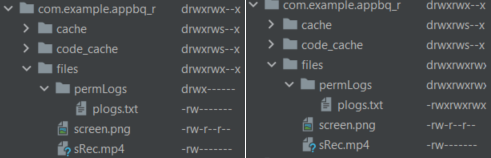
\includegraphics[width=\linewidth]{permnoch}
	\caption{The effect of chmod 777 to folder permissions in Android Device File Explorer.}
	\label{permnoch}
\end{figure}
It results in a permission change for all the folders I specified, but screen.png and sRec.mp4 is unchanged. This persisted even when I made chmod specific to those files. As a last resort, I tried to request \texttt{READ\_EXTERNAL\_STORAGE} permission, but alas, it did not make any difference. In the end, I can say that it is possible to get information from the user with a rooted device, however, accessing those files is another matter.

Unfortunately, the results were the same for the HTC device. Following the same actions did not give a different outcome, and Android device file explorer kept giving the same error for the file.

\chapter{Discussion}
\label{cha:discussion}
In this chapter, findings from the experimentation are discussed. The first section will delve into the overall evolution of the permissions. The next section will draw a comparison on the results.

Before beginning, it is worthwhile to remind that full Android Studio project folders can be found at the following link:
\begin{itemize}
	\item https://github.com/erdemcagri/masterthesis-androidstd/
\end{itemize}

\section{Evolution of permissions}
First, a broad observation of the changes is made, then the specific instances of some differences are explored. One main distinction between versions 4.2.2 and 8.1.0 is the permission groups themselves. To begin with, mentioning groups is unheard of in the papers related to permissions in Android before 2015. This, as pointed out before, is caused by the fact that they don't matter at all. I speculate that the reason permission groups are there is for categorical reasons, providing developers a convenience. Overall, the groups were fairly numerous, since permissions such as calendar, user dictionary, bookmarks, alarm, voicemail got their own groups. In total, permissions declared in the manifest file for 4.2.2 had 25 permission groups, and for 8.1.0, this number was only nine. The normal, or install-time permissions were also flagged under these groups for 4.4.2. The groups for 8.1.0 did not include any install-time permissions, since the permission group feature was strictly adapted for requesting runtime permissions.

While the number of permissions increased greatly with new Android releases, it is observed that this change was done on permissions with protection levels system and signature. The total number of permissions was around 220 for version 4.4.2, and 400 for 8.1.0. In this thesis, the examined protection levels for permissions were normal and dangerous, and no discernable amount could be observed between the versions tested. Naturally, some permissions were added and some were deprecated, or even removed, but the number stayed relatively similar, with 70 permissions declared for 4.4.2 (24 normal and 46 dangerous) , and 69 permissions declared for 8.1.0 (42 normal, and 27 dangerous). One realizes that the main issue here arises from the change in the balance of power between normal and dangerous permissions. The change is almost mirrored across versions where, as time passed, Android reversed the protection levels of some permissions. 

The change includes some permissions being removed. Namely, profile, social stream, user dictionary, history bookmarks, subscribed feeds etc. Android notes that these permissions are removed, but still kept around for backwards compatibility. Thus, their protection levels are switched to normal, regardless of their functionality, and flagged as removed. Depending on what they do, their functionality is either non-functional in the newer versions, or combined with other permissions. The outcome of this was tested with the \texttt{READ\_PROFILE} permission in the AppBQ\_full app. It turned out that \texttt{ContactsContract.Profile} was tied to the \texttt{GET\_ACCOUNTS}. When the \texttt{getProfile()} method from the HTC app was used in the BQ app, it worked as expected. Upon removing the \texttt{GET\_ACCOUNTS} permission, the app crashed. The app also stopped responding when \texttt{READ\_PROFILE} permission was declared. This suggests that the removed permission had no functionality for an app built for version 8.1.0. In this case, the \texttt{AccountManager} and \texttt{ContactsContract.Profile} classes were tied to the same permission, whereas before they were associated with their respective permissions. The implication here is clear, as Zhauniarovic et al. argued, Android permissions moved into a more coarse-grained arrangement over time, when instead, scholars such as Fang et al. were asking for a more fine-grained structure even before version 6.0.

A certain number of permissions were demoted, as in, their protection levels were changed from dangerous to normal, making them install-time permissions. Notable instances include \texttt{INTERNET}, \texttt{BLUETOOTH}, \texttt{BLUETOOTH\_ADMIN}, and \texttt{NFC}. The implications of this will be discussed in the next section.

\section{Comparison of results}
Although it is quite difficult to justify a long list of permissions being declared to the user, the full permission state of the apps were made to gauge the extent of confidential information a developer could extract from the user, for giving an overall picture of the whole scheme, and to demonstrate said information by permissions of which it is bound to. However, as noted in Section 3.1, application overprivilege is a problem in the Android ecosystem which makes drawing a distinguishing picture of the user easier.

Since the experiments were tied to the confidentiality scope, the results between the BQ and HTC devices are nearly similar. The major difference is between the permissions themselves, but not the methods that were used to extract information. In the BQ device, the permissions are coarse-grained, as in one permission holds the key to more obtainable confidential information. It is evident why Google moved in such a direction, their aim was to keep the new permission request concept pristine and unsophisticated to the end-user, and having fewer buttons to touch, enabled this aim. If they kept the same grouping of permissions in the post 6.0 era, the user would have to tap 25 times over and over again to give access to the dangerous runtime permissions in my app. Nevertheless, no app should request all permissions available in actuality. In addition, the requests should definitely not be made upon first launch, considering this would overwhelm the majority of the users, and consequently less attention would be given out. The preferable approach is to request a permission at the point in time when the app needs the specific resource, thus allowing the user to give their attention to only the matter at hand.

One notable, and positive difference between the apps concerns the device hardware identifiers, specifically, device MAC addresses for Wi-Fi and Bluetooth modems. After 6.0, Android effectively blocks all access to these addresses, which means that even with full permissions, developers cannot obtain this information. On the other hand, if one remembers the wide OS version distribution for the Android ecosystem, the context somewhat differs. The case is the same for the IMEI and IMSI values, where these are blocked to the developers, but only for devices that have the version (and beyond) when this block was introduced. For both test devices, the new and the old, IMEI and IMSI values are available provided one declares the telephony permission. A device with as recent release date as three years ago, is considerably less secure than a device that came one year after. To Android's benefit, at least in the Android Studio IDE, when one tries to extract this information, it results in an error. Although this error acts as a mere warning for developers with apps with smaller minimum SDK value than the specified API level. The minimum SDK value denotes the minimum version of the Android OS required to run an app. This means that even a brand-new application is able to obtain said information, if the app \textit{can} run on devices with versions that came before the block. It is worth mentioning a limitation of this master thesis. Considering the hectic and haphazard version updates of Android, the test devices used could not picture the wide variety of devices actively in use in the ecosystem. Although they are outdated, this by no means indicates that they are not in use. 

The installation process, at least the information presented to the user upon install, differs on a fundamental level between the applications. In HTC, when the installation is initialized, the user gets asked a prompt about whether or not to install the application. Between this question and the install button, stands a list that includes every permission (by their readable descriptions). This does not differ if the app asks for only normal permissions, dangerous permissions, or both. The prompt plainly lists everything, in every case. It goes without saying that such a manner of operation was not perfect; the user could get overwhelmed, and although they could inspect the list in the Settings, they could not revoke any permissions. If the user wanted to install the app, they simply had to live with the fact that whatever the app wants, the app gets. Then, Google released this new version called Marshmallow, which introduced permission requests at runtime and much more. Did it fix the aforementioned issues? Well, saying \textit{not exactly} would be an understatement. The new version, for some reason, got rid of the permission list during the installation prompt. On top of that, after asking whether the user is willing to install the app or not, the prompt states the following: "It does not require any special access.".  For a post-6.0 OS version device, I could not see any way for the app to declare \textit{special access} in the installation prompt. Whether the app had install-time permissions, runtime permissions, both, or even root command executions, the app at the prompt stated that it did not need special access. Let us forget the install-time permissions, obviously, the app did not have any access to the dangerous runtime permissions during installation. However, it is fair to assume that if the app declared these permissions, it would also request them. Even if these permissions are revokable, it is my opinion that the app should notify the user up front. The app should never claim that no special access is needed, even if only one permission is declared, regardless of protection level. Furthermore, if only the install-time permissions are declared in the manifest file, the user has in no way of viewing these permissions, neither upon installation, nor in the Settings. It is beyond my reasoning that install-time permissions are visible in the Settings when declared alongside runtime permissions, but invisible when they are declared by themselves. They should never be invisible. This way, I declared 42 permissions without any user knowledge. Certainly majority of these permissions were deserving of their protection levels, but a few can make the difference, especially when non-revokable and invisible \texttt{INTERNET} permission is listed among this select few. 

Without any user notification, the BQ app with no runtime permissions was able to obtain previously paired BT device names and MAC addresses, and previously connected Wi-Fi networks. Interestingly, the MAC addresses of these Wi-Fi networks were locked behind location permissions, but Bluetooth device MAC addresses were not. The location lock is interesting, since the Wi-Fi and Bluetooth-related permissions were dangerous before 6.0, and their protection levels were reverted to normal after this. With it, configured Wi-Fi network MAC addresses, currently connected Wi-Fi network, Wi-Fi scan, and Bluetooth discovery processes only return valid values with a runtime location permission, thus needs to be requested from the user. However, even after years passed, this change still comes off as unnecessarily convoluted. Why remove configured Wi-Fi MAC addresses but keep paired Bluetooth MAC addresses available? Why remove connected Wi-Fi network name but keep information such as RSSI and link speed accessible? I am not debating the information block from the developer. But the reasoning is not clear. It is done in a way that is unfriendly to the user, if the information wanted to be blocked, the Wi-Fi and Bluetooth permissions should have remained as dangerous runtime permissions, so the user would have known the nature of the requested information. An attacker can gather information on the previously connected Wi-Fi networks and paired Bluetooth devices, store it in the device using shared preferences or database APIs, thus construct a partial fingerprint of the user. In addition, they can even upload it to a server in the cloud, since the \texttt{INTERNET} permission is also turned into a normal permission. The mirroring HTC app could have no permissions, since the user was notified of any permissions declared with a prompt upon install. The only information obtained was related to the device manufacturer, model, and serial, which is not specific to the user (but can be in a small pool of Android users), and Android ID, which is randomly changed on factory reset and OS version change on some devices.

\chapter{Conclusion}
\label{cha:conclusion}

This master thesis had set out to investigate Android permission scheme from a confidentiality-aware perspective. The main aim was to determine information leakages pertaining to the device user and their immediate environment. The overview of the Android permission scheme and literature review was fundamental steps to comprehend the context of which the experimentation took place.

The investigation was conducted with two devices from different time periods in reference to the Android platform. The device user point of view was integral in the development of test applications where user awareness was the main consideration. One test case disregarded this user-awareness, and aimed to demonstrate the extent of information that could be gathered. The other test case emphasized zero user-awareness, where they one could not detect any permission was declared and/or information being gathered.

One must provide nuance to the interpretation of the results, they can neither be quantified, nor construed as wholly good or bad. The runtime permission addition to the overall scheme was essential, and Google's incorporation of this function into the platform was long overdue. While the two devices from different time points opened a window to this overhaul, the work of Zhauniarovich and Gadyatskaya reveal the rocky start of this update, which filled the gaps that I could not. Initially, it is observed that this necessary update did not result in a positive outcome from a security perspective. Nonetheless, from the version 6.0 to the 8.1.0, there were notable improvements on the whole. In addition, from the thesis observation point of 8.1.0 and onward, there were also incremental advancements to the security. Due to the version discrepancy in the general market, these refinements do not manifest itself to every device that is actively in use. It is my opinion that one can infer an overall trend of positivity, but the current situation is inadequate in terms of security, and Google is all too slow (or simply unable) to mend the issues at hand. Evidently, the nature of Android does not allow for an overarching solution, yet. Whether the status quo will change or not, only future research on the matter can shed light on it.

%end this par with two step forward and one step back
%some stuff did not fit the scope, integrity etc

%mention for future work small changes android makes, will be interesting etc, future study can increase device size

\printbibliography

%\appendix
%\chapter{Appendix}
%Full program codes, manifest and output files can also be found in the following GitHub page.

%\section{AppBQ\_full/MainActivity.java}
%\lstinputlisting{./code/bqf-MainActivity.java}

%\section{AppBQ\_none/MainActivity.java}
%\lstinputlisting{./code/bqn-MainActivity.java}

%\section{AppHTC\_full/MainActivity.java}
%\lstinputlisting{./code/htcf-MainActivity.java}

%\section{AppHTC\_none/MainActivity.java}
%\lstinputlisting{./code/htcn-MainActivity.java}
\end{document}
